\documentclass[10pt]{article}

% Load commands & pakcages
% THESIS VERSION

%%%% PACKAGES %%%%
\usepackage{graphicx}
% \usepackage{epstopdf}
\usepackage{array}
\newcommand{\PreserveBackslash}[1]{\let\temp=\\#1\let\\=\temp}
\newcolumntype{C}[1]{>{\PreserveBackslash\centering}p{#1}}
\newcolumntype{R}[1]{>{\PreserveBackslash\raggedleft}p{#1}}
\newcolumntype{L}[1]{>{\PreserveBackslash\raggedright}p{#1}}
\usepackage{lastpage}
\usepackage{fancyhdr}
\let\openbox\relax
\usepackage{amsmath}
\usepackage{amssymb,amsthm,amsfonts}
\allowdisplaybreaks
\usepackage{upgreek}
\usepackage{bm}
\usepackage{algorithm}
\usepackage{algpseudocode}
\usepackage{relsize}
% \usepackage{dashbox}%
\usepackage{wasysym}

\usepackage[utf8]{inputenc}

% Tables
\usepackage{hhline}
\usepackage[version=4]{mhchem}
\usepackage{siunitx}
\usepackage{longtable,tabularx}
\setlength\LTleft{0pt} 

\usepackage{hyperref}
\hypersetup{
    colorlinks=true,
    linkcolor=black,
    filecolor=black, 
    citecolor=black,     
    urlcolor=blue,
}
\usepackage{float}
\usepackage{adjustbox}
\usepackage{subfig}
\usepackage{mathtools}
% \usepackage{units}
% \usepackage{enumitem}

% Colors
\usepackage{xcolor}
% \definecolor{brickred}{rgb}{0.8, 0.25, 0.33}
\definecolor{alizarin}{rgb}{0.82, 0.1, 0.26}

% For shaded boxes
% \usepackage{framed}
% \usepackage[svgnames]{xcolor}
% %\colorlet{shadecolor}{LavenderBlush3}
% %\colorlet{shadecolor}{gray!20}
% \colorlet{shadecolor}{blue!12}

\makeatletter
\newcommand{\leqnomode}{\tagsleft@true\let\veqno\@@leqno}
\newcommand{\reqnomode}{\tagsleft@false\let\veqno\@@eqno}
\makeatother

\newcommand\blfootnote[1]{%
  \begingroup
  \renewcommand\thefootnote{}\footnote{#1}%
  \addtocounter{footnote}{-1}%
  \endgroup
}

%%%% COMMANDS %%%%

% Editing
\definecolor{commentgreen}{RGB}{0, 153, 0}
\definecolor{highlightred}{RGB}{153,0,0}
\newcommand{\todo}[1]{{\color{blue}(TODO: #1)}}
\newcommand{\comment}[1]{{\color{blue} #1}}
\newcommand{\remove}[1]{{\color{red} \sout #1 }}
\newcommand{\addin}[1]{{\color{commentgreen} #1}}
\newcommand{\highlight}[1]{{\color{highlightred} #1}}
\newcommand{\sref}[1]{\S\ref{#1}}
\newcommand{\pref}[1]{Problem~\ref{#1}}
\newcommand{\fref}[1]{Figure~\ref{#1}}
\newcommand{\chref}[1]{Chapter~\ref{#1}}
\newcommand{\aref}[1]{Appendix~\ref{#1}}
\newcommand{\thmref}[1]{Theorem~\ref{#1}}
\newcommand{\tabref}[1]{Table~\ref{#1}}

% Tables
\newcommand{\tabspace}{\hspace{-0.35cm}}
\newcommand{\tabsep}{\null\hspace{0.5cm}\null}

% Number/Set stuff
\newcommand{\real}{{\mathbb{R}}}
\newcommand{\realp}{\real_+}
\newcommand{\realpp}{\real_{++}}
\newcommand{\complex}{{\mathbb{C}}}
\newcommand{\field}{{\mathbb{F}}}
\newcommand{\realpart}{\mathrm{Re}}
\newcommand{\impart}{\mathrm{Im}}
\newcommand{\psd}[1]{\mathbb{S}^{#1}_+}
\newcommand{\pd}[1]{\mathbb{S}^{#1}_{++}}
\newcommand{\ispd}{\succ~0}
\newcommand{\ispsd}{\succeq~0}
\newcommand{\setdom}{\mathcal{D}}
\newcommand{\coneK}{\mathcal{K}}
\newcommand{\lcone}[1]{\real_+^{#1}}
\newcommand{\qcone}[1]{\mathcal{Q}^{#1}}
\newcommand{\conleq}{\preceq_{\coneK}}
\newcommand{\congeq}{\succeq_{\coneK}}
\newcommand\something[1][H]{\setlength{\fboxsep}{0pt}\setlength{\dashlength}{2.2pt}\setlength{\dashdash}{1.1pt} \dbox{\phantom{#1}}}
% \newcommand{\something}{\dashedph}

% Derivatives & Optimization
\newcommand{\argmin}{\operatorname{argmin}}
\newcommand{\der}[2]{\frac{d #1}{d #2}}
\newcommand{\pder}[2]{\frac{\partial #1}{\partial #2}}
\newcommand{\sproc}{$\mathcal{S}$-procedure }
\newcommand{\scvx}{\texttt{SCvx}}

% Optimal Control
\newcommand{\lj}{\lambda^0}
\newcommand{\lm}{\lambda_m}
\newcommand{\lr}{\bm{\lambda}_r}
\newcommand{\lv}{\bm{\lambda}_v}
\newcommand{\lt}{\lambda_{\theta}}
\newcommand{\lw}{\lambda_{\omega}}
\newcommand{\costate}{\bm{\lambda}}
\newcommand{\p}{\hat{\costate}}
\newcommand{\dlm}{\dot{\lambda}_m}
\newcommand{\dlr}{\dot{\bm{\lambda}}_r}
\newcommand{\dlv}{\dot{\bm{\lambda}}_v}
\newcommand{\dlt}{\dot{\lambda}_{\theta}}
\newcommand{\dlw}{\dot{\lambda}_{\omega}}
\newcommand{\cw}{c_{\omega}}
\newcommand{\lri}{\bm{\lambda}_{r,0}}
\newcommand{\lvi}{\bm{\lambda}_{v,0}}
\newcommand{\setB}{\mathcal{B}}
\newcommand{\setU}{\mathcal{U}}
\newcommand{\setX}{\mathcal{X}}
\newcommand{\setI}{\mathcal{I}}
\newcommand{\setGen}{\mathcal{C}}
\newcommand{\term}{M}
\newcommand{\runn}{L}
\newcommand{\primer}{\bm{p}}

% Coordinate frames
\newcommand{\inertial}{\mathcal{I}}
\newcommand{\body}{\mathcal{B}}
\newcommand{\landing}{\mathcal{L}}
\newcommand{\fixed}{\mathcal{F}}
\newcommand{\cframe}[1]{\mathcal{F}_{#1}}
\newcommand{\Fbody}{\cframe{\body}}
\newcommand{\Finertial}{\cframe{\inertial}}
\newcommand{\Fecef}{\cframe{\fixed}}
\newcommand{\Flanding}{\cframe{\landing}}
\newcommand{\DCM}[2]{C_{{#2} \leftarrow {#1}}}
\newcommand{\cIB}{C_{\body \leftarrow \inertial}}
\newcommand{\cBI}{C_{\inertial \leftarrow \body}}
\newcommand{\cLB}{C_{\body \leftarrow \landing}}
\newcommand{\cBL}{C_{\landing \leftarrow \body}}
\newcommand{\cBO}{C_{\landing\,\body}}
\newcommand{\cIF}{C_{\inertial\,\fixed}}
\newcommand{\cFI}{C_{\fixed\,\inertial}}
\newcommand{\xI}{\bm{x}_{\inertial}}
\newcommand{\yI}{\bm{y}_{\inertial}}
\newcommand{\zI}{\bm{z}_{\inertial}}
\newcommand{\xF}{\bm{x}_{\fixed}}
\newcommand{\yF}{\bm{y}_{\fixed}}
\newcommand{\zF}{\bm{z}_{\fixed}}
\newcommand{\xB}{\bm{x}_{\body}}
\newcommand{\yB}{\bm{y}_{\body}}
\newcommand{\zB}{\bm{z}_{\body}}
\newcommand{\xL}{\bm{x}_{\landing}}
\newcommand{\yL}{\bm{y}_{\landing}}
\newcommand{\zL}{\bm{z}_{\landing}}
\newcommand{\ex}{\bm{e}_x}
\newcommand{\ey}{\bm{e}_y}
\newcommand{\ez}{\bm{e}_z}
\newcommand{\eu}{\bm{e}_u}

% General math
\newcommand{\eps}{\epsilon}
\newcommand{\dg}{^{\circ}}
\newcommand{\blkdiag}{\mathop{\bf blkdiag}}
\newcommand{\spec}[1]{\mathop{\bf spec}\left\lbrace #1 \right\rbrace}
\newcommand{\diag}[1]{\mathop{\bf diag}\left\lbrace #1 \right\rbrace}
\newcommand{\eye}[1]{I_{#1}}
\newcommand{\zeros}[2]{0_{#1 \times #2}}
\newcommand{\ones}[1]{\bm{1}_{#1}}
\newcommand{\dom}[1]{\mathop{\bf dom} #1}
\newcommand{\eig}[1]{\mathop{\bf eig}\left\lbrace #1 \right\rbrace}
\newcommand{\hamil}{\mathcal{H}}
\newcommand{\sign}[1]{\mathop{sign}\left( #1 \right)}
\newcommand{\inv}[1]{ #1^{-1}}
\newcommand{\definedas}{\coloneqq}
\newcommand{\unit}[1]{\mathrm{#1}}
\newcommand{\tran}{^{\top}}
\newcommand{\jacob}[2]{\nabla_{#2}{#1}}
\newcommand{\jacobev}[3]{\jacob{#1}{#2}\big(#3\big)}
\newcommand{\hess}[3]{\nabla_{#2#3}{#1}}
\newcommand{\ip}{\boldsymbol{\cdot}}
\newcommand{\ipQ}{\boldsymbol{\cdot}}
\newcommand{\ipDQ}{\mathrel{\raisebox{1pt}{\scalebox{0.6}{$\circ$}}}}
\newcommand{\twonorm}[1]{\|#1\|_2}
\newcommand{\onenorm}[1]{\|#1\|_1}
\newcommand{\infnorm}[1]{\|#1\|_{\infty}}
\newcommand{\pnorm}[1]{\|#1\|_p}

% Time
\newcommand{\tpu}{t_{\text{pu}}}
\newcommand{\tf}{t_f}
\newcommand{\tfmin}{t_{f,\min}}
\newcommand{\tfmax}{t_{f,\max}}
\newcommand{\ti}{t_0}
\newcommand{\tc}{t_c}
\newcommand{\tb}{t_b}

% Physical parameters
\newcommand{\gI}{\bm{g}_{\inertial}}
\newcommand{\gB}{\bm{g}_{\body}}
\newcommand{\gL}{\bm{g}_{\landing}}
\newcommand{\dqgI}{\dq{g}_{\inertial}}
\newcommand{\dqgB}{\dq{g}_{\body}}
\newcommand{\J}{\bm{J}}
\newcommand{\Ca}{C_{A}}
\newcommand{\CaI}{C_{A,\inertial}}
\newcommand{\Sa}{S_{A}}
\newcommand{\setaero}{\mathcal{A}(V)}
\newcommand{\rCPB}{\bm{r}_{\textit{cp}}}
\newcommand{\density}{\rho}
\newcommand{\Pamb}{P_{\textit{amb}}}
\newcommand{\mell}{\bm{\ell}}

% MASS
% continuous
\newcommand{\m}{m}
\newcommand{\mf}{\m(\tf)}
\newcommand{\mic}{\m_{\textit{ic}}}
% discrete
\newcommand{\mk}{\m_{k}}
\newcommand{\mi}{\m_0}
\newcommand{\mN}{\m_N}
\newcommand{\cv}{{c^*}}

% continuous
\newcommand{\rI}{\bm{r}_{\inertial}}
\newcommand{\rIb}{\bar{\bm{r}}_{\inertial}}
\newcommand{\rB}{\bm{r}_{\body}}
\newcommand{\rL}{\bm{r}_{\landing}}
\newcommand{\rBb}{\bar{\bm{r}}_{\body}}
\newcommand{\rIdot}{\dot{\bm{r}}_{\inertial}}
\newcommand{\rLdot}{\dot{\bm{r}}_{\landing}}
\newcommand{\ric}[1]{\bm{r}_{#1,\textit{ic}}}
% discrete
\newcommand{\rk}[1]{\bm{r}_{#1,\ind}}
\newcommand{\ri}[1]{\bm{r}_{#1,0}}
\newcommand{\rf}[1]{\bm{r}_{#1,f}}
\newcommand{\rN}[1]{\bm{r}_{#1,N}}
\newcommand{\prig}{\bm{b}_{\bm{r},0}}

% VELOCITY
% continuous
\newcommand{\vI}{\bm{v}_{\inertial}}
\newcommand{\vB}{\bm{v}_{\body}}
\newcommand{\vL}{\bm{v}_{\landing}}
\newcommand{\vBdot}{\dot{\bm{v}}_{\body}}
\newcommand{\vIb}{\bar{\bm{v}}_{\inertial}}
\newcommand{\vBb}{\bar{\bm{v}}_{\body}}
\newcommand{\vIdot}{\dot{\bm{v}}_{\inertial}}
\newcommand{\vLdot}{\dot{\bm{v}}_{\landing}}
\newcommand{\vic}[1]{\bm{v}_{#1,\textit{ic}}}
% discrete
\newcommand{\vk}[1]{\bm{v}_{#1,\ind}}
\newcommand{\vi}[1]{\bm{v}_{#1,0}}
\newcommand{\vf}[1]{\bm{v}_{#1,f}}
\newcommand{\vN}[1]{\bm{v}_{#1,N}}
\newcommand{\pvig}{\bm{b}_{\bm{v},0}}

% ANGULAR VELOCITY
% continuous
\newcommand{\w}{\bm{\omega}}
\newcommand{\wB}{\w_{\body}}
\newcommand{\wBdot}{\dot{\w}_{\body}}
\newcommand{\wBb}{\bar{\w}_{\body}}
\newcommand{\wic}{\w_{\body,\textit{ic}}}
%discrete
\newcommand{\wk}{\w_{\body,\ind}}
\newcommand{\wi}{\w_{\body,0}}
\newcommand{\wf}{\w_{\body,f}}
\newcommand{\wN}{\w_{\body,N}}

% CONTROLS
\newcommand{\FI}{\bm{F}_{\inertial}}
\newcommand{\FB}{\bm{F}_{\body}}
\newcommand{\MB}{\bm{M}_{\body}}

\newcommand{\uB}{\bm{u}_{\body}}
\newcommand{\uI}{\bm{u}_{\inertial}}
\newcommand{\uL}{\bm{u}_{\landing}}
\newcommand{\ui}[1]{\bm{u}_{#1,0}}
\newcommand{\uk}[1]{\bm{u}_{#1,\ind}}
\newcommand{\uf}[1]{\bm{u}_{#1,f}}
\newcommand{\uBb}{\bar{\bm{u}}_{\body}}
\newcommand{\duB}{\dot{\bm{u}}_{\body}}
\newcommand{\duBk}{\dot{\bm{u}}_{\body,\ind}}

\newcommand{\tauI}{\bm{\tau}_{\inertial}}
\newcommand{\tauIb}{\bar{\bm{\tau}}_{\inertial}}
\newcommand{\tauB}{\bm{\tau}_{\body}}
\newcommand{\tauBb}{\bar{\bm{\tau}}_{\body}}
\newcommand{\taui}[1]{\bm{\tau}_{#1,0}}
\newcommand{\tauk}[1]{\bm{\tau}_{#1,k}}
\newcommand{\tauf}[1]{\bm{\tau}_{#1,f}}

% FORCES
\newcommand{\aero}{\bm{A}}
\newcommand{\aeroB}{\aero_{\body}}
\newcommand{\aeroI}{\aero_{\inertial}}
\newcommand{\aeroL}{\aero_{\landing}}

\newcommand{\ru}{\bm{r}_{u}}
\newcommand{\umag}{\Gamma}
\newcommand{\udir}{\bm{d}}
\newcommand{\Isp}{I_{\text{sp}}}

% DERIVATIVES
\newcommand{\dFdx}[3]{\pder{F}{\bm{x}}\biggr|_{#1,#2,#3}}
\newcommand{\dFdu}[3]{\pder{F}{\bm{u}}\biggr|_{#1,#2,#3}}
\newcommand{\dFds}[3]{\pder{F}{\sigma}\biggr|_{#1,#2,#3}}
\newcommand{\mdot}{\dot{m}}
\newcommand{\rdot}{\dot{\bm{r}}_{\inertial}}
\newcommand{\vdot}{\dot{\bm{v}}_{\inertial}}
\newcommand{\thetadot}{\dot{\theta}}
\newcommand{\dw}{\dot{\omega}}
\newcommand{\wdot}{\dot{\bm{\omega}}_{\body}}

% constraints
\newcommand{\mwet}{m_{\text{wet}}}
\newcommand{\mdry}{m_{\text{dry}}}
\newcommand{\vmax}{v_{\max}}
\newcommand{\wmax}{\omega_{\max}}
\newcommand{\gimbal}{\delta}
\newcommand{\gimbalmax}{\delta_{\max}}
\newcommand{\los}{\xi}
\newcommand{\losmax}{\los_{\max}}
\newcommand{\losf}{c_l}
\newcommand{\losvec}{\bm{p}_{\body}}
\newcommand{\rLoSI}{\bm{r}_{d,\inertial}}
\newcommand{\rLoSB}{\bm{r}_{d,\body}}
\newcommand{\gs}{\gamma}
\newcommand{\gsmax}{\gamma_{\max}}
\newcommand{\gsvec}{\zI}
\newcommand{\gsf}{c_g}
\newcommand{\gsM}{M_g}
\newcommand{\tiltmax}{\theta_{\max}}
\newcommand{\tilt}{\theta}
\newcommand{\tiltf}{c_t}
\newcommand{\tiltM}{M_t}
\newcommand{\aoa}{\alpha}
\newcommand{\aoamax}{\alpha_{\max}}
\newcommand{\Gmin}{\Gamma_{\min}}
\newcommand{\Gmax}{\Gamma_{\max}}
\newcommand{\umin}{u_{\min}}
\newcommand{\umax}{u_{\max}}
\newcommand{\taumax}{\tau_{\max}}
\newcommand{\dTmax}{\dot{T}_{\max}}
\newcommand{\dumax}{\dot{\bm{u}}_{\max}}
\newcommand{\dgimmax}{\dot{\gimbal}_{\max}}

% State-triggered Constraints
\newcommand{\stcz}{\bm{z}}
\newcommand{\stcnz}{n_z}
\newcommand{\stcs}{\sigma}
\newcommand{\stcshat}{\hat{\stcs}}
\newcommand{\stcg}{g}
\newcommand{\stcng}{n_g}
\newcommand{\stcc}{c}
\newcommand{\stcnc}{n_c}
\newcommand{\stch}{h}
\newcommand{\stca}{\varepsilon}
\newcommand{\gaoa}{g_{\aoa}}
\newcommand{\caoa}{c_{\aoa}}
\newcommand{\haoa}{h_{\aoa}}
\newcommand{\vlim}{V_{\text{lim}}}
\newcommand{\modeset}{\mathcal{A}}

% Quaternions & dual quaternions
\newcommand{\setq}{\mathbb{Q}}
\newcommand{\setuq}{\setq_u}
\newcommand{\setuqR}{\real_{u}^4}
\newcommand{\setqv}{\setq_v}
\newcommand{\setdq}{\widetilde{\setq}}
\newcommand{\setudq}{\setdq_u}
\newcommand{\setudqR}{\real_{u}^8}
\newcommand{\quat}[1]{\bm{#1}}
\newcommand{\quatv}[1]{\bm{#1}_v}
\newcommand{\quats}[1]{{#1}_4}
\newcommand{\q}{\bm{q}}
\newcommand{\qid}{\q_{\text{id}}}
\newcommand{\qv}{\q_v}
\newcommand{\qs}{q_4}
\newcommand{\qi}{\q_0}
\newcommand{\qk}{\q_{\ind}}
\newcommand{\qN}{\q_N}
\newcommand{\qIB}{\q_{\body \leftarrow \inertial}}
\newcommand{\qic}{\q_\textit{ic}}
\newcommand{\qf}{\q_\textit{f}}
\newcommand{\qb}{\bar{\q}}
\newcommand{\qbi}{\bar{\q}_0}
\newcommand{\qdot}{\dot{\q}}
\newcommand{\dq}[1]{\tilde{\bm{#1}}}
\newcommand{\dqq}{\dq{q}}
\newcommand{\dqb}{\bar{\dqq}}
\newcommand{\dqw}{\dq{\omega}}
\newcommand{\dqwdot}{\dot{\dq{\omega}}}
\newcommand{\dqqic}{\dqq_{\textit{ic}}}
\newcommand{\dqqi}{\dqq_0}
\newcommand{\dqqk}{\dqq_{\ind}}
\newcommand{\dqqN}{\dqq_N}
\newcommand{\dqqf}{\dqq_f}
\newcommand{\dqwic}{\dqw_{\textit{ic}}}
\newcommand{\dqwi}{\dqw_0}
\newcommand{\dqwk}{\dqw_{\ind}}
\newcommand{\dqwN}{\dqw_{N}}
\newcommand{\dqwf}{\dqw_f}
\newcommand{\dqx}{\dq{x}}
\newcommand{\dqu}{\dq{u}}
\newcommand{\dqdot}[1]{\dot{\tilde{\bm{#1}}}}
\newcommand{\qskew}[1]{[ #1 ]_{\otimes}}
\newcommand{\qskewstar}[1]{[ #1 ]_{\otimes}^*}
\newcommand{\qcross}[1]{ [ #1 ]_{\oslash}}
\newcommand{\qcrossstar}[1]{ [ #1 ]_{\oslash}^*}
\newcommand{\It}{\tilde{\bm{I}}_8}
\newcommand{\dqqig}{\bm{b}_{\dqq}}
\newcommand{\dqwig}{\bm{b}_{\dqw}}
\newcommand{\dqaero}{\dq{\aero}}

% Optimization & successive
\newcommand{\ind}{i}
\newcommand{\Jthree}{J_{3-\text{DoF}}}
\newcommand{\Jsix}{J_{6-\text{DoF}}}
\newcommand{\Jpp}{J_{\text{pinpoint}}}
\newcommand{\Jsoft}{J_{\text{soft-land}}}
\newcommand{\Jminerr}[1]{J_{\text{min-error},#1}}
\newcommand{\Jtr}{J_{\text{tr}}}
\newcommand{\Jvc}{J_{\text{vc}}}
\newcommand{\xx}{\bm{x}}
\newcommand{\XX}{\bm{X}}
\newcommand{\uu}{\bm{u}}
\newcommand{\UU}{\bm{U}}
\renewcommand{\ss}{s}
\renewcommand{\SS}{S}
\newcommand{\zz}{\bm{z}}
\newcommand{\sig}{\sigma}
\newcommand{\xb}{\bar{\xx}}
\newcommand{\ub}{\bar{\uu}}
\newcommand{\sigb}{\bar{\sig}}
\renewcommand{\sb}{\bar{s}}
\newcommand{\zb}{\bar{\zz}}
\newcommand{\ww}{R}
\newcommand{\dummy}{\zeta}
\newcommand{\ee}{\bm{\eta}}
\newcommand{\eek}{\eta_{\ind}}
\newcommand{\eet}{\eta_{s}}
\newcommand{\vv}{\bm{\nu}}
\newcommand{\VV}{\bm{V}}
\newcommand{\wtr}{\bm{w}_{\text{tr}}}
\newcommand{\wtrk}{\bm{w}_{\text{tr},\ind}}
\newcommand{\wvc}{w_{\text{vc}}}
\newcommand{\res}{\Delta}
\newcommand{\resk}{\res_\ind}
\newcommand{\reskp}{\res_{\ind+1}}
\newcommand{\resmin}{\res_{\min}}
\newcommand{\setK}{\mathsf{N}}
\newcommand{\setKb}{\bar{\mathsf{N}}}
\newcommand{\dxtol}{\delta x_{\text{tol}}}
\newcommand{\err}{\varepsilon}
\newcommand{\wv}{w_{\nu}}
\newcommand{\xxic}{\xx_{\textit{ic}}}
\newcommand{\xxf}{\xx_{\textit{f}}}

% Scaling
\newcommand{\Px}{P_x}
\newcommand{\Pu}{P_u}
\newcommand{\qx}{\bm{p}_x}
\newcommand{\qu}{\bm{p}_u}
\newcommand{\Pt}{p_t}
\newcommand{\Pz}{P_z}
\newcommand{\qz}{\bm{p}_z}
\newcommand{\scale}[1]{\hat{#1}}
\newcommand{\xxs}{\scale{\xx}}
\newcommand{\xxbs}{\scale{\xb}}
\newcommand{\uubs}{\scale{\ub}}
\newcommand{\uus}{\scale{\uu}}
\newcommand{\sss}{\scale{\ss}}
\newcommand{\ees}{\scale{\ee}}
\newcommand{\eets}{\hat{\eta}_{s}}
\newcommand{\eeks}{\scale{\eta}_{\ind}}
\newcommand{\XXs}{\scale{\XX}}
\newcommand{\UUs}{\scale{\UU}}
\newcommand{\VVs}{\scale{\VV}}
\newcommand{\zzs}{\scale{\zz}}

% LOCAL FEASIBILITY
\newcommand{\sigI}{\Sigma_0}
\newcommand{\sigF}{\Sigma_f}
\newcommand{\xe}{\bm{\upchi}}
\newcommand{\xek}{\xe_{\ind}}
\newcommand{\xeic}{\xe_{\textit{ic}}}
\newcommand{\xef}{\xe_f}
\newcommand{\xeN}{\xe_N}
\newcommand{\ue}{\bm{\mu}}
\newcommand{\uek}{\ue_{\ind}}
\newcommand{\se}{\varsigma}
\newcommand{\expt}[1]{\mathbb{E}\big[#1\big]}

% SATELLITE GNC
\newcommand{\sI}{\bm{s}_{\inertial}}
\newcommand{\bB}{\bm{b}_{\body}}
\newcommand{\bI}{\bm{b}_{\inertial}}
\newcommand{\pang}{\theta}
\newcommand{\hB}{\bm{h}_{\body}}
\newcommand{\dhB}{\dot{\bm{h}}_{\body}}
\newcommand{\hBic}{\bm{h}_{\body,\textit{ic}}}
\newcommand{\hBf}{\bm{h}_{\body,\textit{f}}}
\newcommand{\hw}{\bm{h}_w}
\newcommand{\dhw}{\dot{\bm{h}}_w}
\newcommand{\hwic}{\bm{h}_{w,\textit{ic}}}
\newcommand{\hwf}{\bm{h}_{w,\textit{f}}}
\newcommand{\Hq}{H_{\q}}
\newcommand{\Hw}{H_{\omega}}
\newcommand{\ME}{\tilde{M}_e}
\newcommand{\MI}{\tilde{M}_i}

% astrodynamics
\renewcommand{\sun}{\astrosun}
\renewcommand{\earth}{\oplus}
\newcommand{\moon}{\leftmoon}

%% theorems and stuff

\newtheorem{theorem}{Theorem}[section]
\newtheorem{assumption}[theorem]{Assumption}
\newtheorem{remark}[theorem]{Remark}
\newtheorem{proposition}{Proposition}
\newtheorem{constraint}{Constraint}
\newtheorem{assume}{Assumption}
\newtheorem{problem}{Problem}

% \newtheorem{theorem}{Theorem}[section]
% \newtheorem{definition}{Definition}
% \newtheorem{assumption}[theorem]{Assumption}
% \newtheorem{lemma}[theorem]{Lemma}
% \newtheorem{claim}[theorem]{Claim}
% \newtheorem{remarks}[theorem]{Remarks}
% \newtheorem{remark}[theorem]{Remark}
% \newtheorem{example}[theorem]{Example}
% \newtheorem{corollary}[theorem]{Corollary}
% \newtheorem{proposition}{Proposition}
% \newtheorem{constraint}{Constraint}
% \newtheorem{problem}{Problem}
% \newtheorem{assume}{Assumption}

% Other
\newcommand*\samethanks[1][\value{footnote}]{\footnotemark[#1]}
\newcommand{\eqnref}[1]{(\ref{#1})}
\newcommand{\class}[1]{\texttt{#1}}
\newcommand{\package}[1]{\texttt{#1}}
\newcommand{\file}[1]{\texttt{#1}}
\newcommand{\BibTeX}{\textsc{Bib}\TeX}
\newcommand{\code}[1]{\texttt{#1}}
\newcommand{\ttt}[1]{\texttt{#1}}

\newcommand{\quotebox}[1]{
	\begin{shaded*}
	\vspace{-3pt}
	\begin{center}
	\textit{#1}
	\end{center}
	\vspace{-3pt}
	\end{shaded*}
}
\usepackage{rotating}
\usepackage{tikz}
\usepackage{pgfplots}
\usepackage{ifthen}
\pgfplotsset{compat=1.12}
\usetikzlibrary{calc}
\usetikzlibrary{patterns}
\usetikzlibrary{decorations.pathmorphing,decorations.markings}
\usetikzlibrary{math}
\usetikzlibrary{scopes}
\usetikzlibrary{fadings}
\usetikzlibrary{arrows}
\usetikzlibrary{arrows.meta}
\tikzset{>=latex}

\pgfdeclarelayer{bg}    % declare background layer
\pgfsetlayers{bg,main}  % set the order of the layers (main is the standard layer)

\definecolor{beige}{RGB}{245,245,220}
\definecolor{darkred}{rgb}{0.90,0.00,0.00}%red}%!75!black!100}
\definecolor{darkgreen}{rgb}{0.00,0.45,0.00}

\definecolor{ucol}{RGB}{255,0,0}
\definecolor{gcol}{RGB}{0,120,0}
\definecolor{scol}{RGB}{63, 226, 45}
\definecolor{vcol}{RGB}{0,0,0}
\definecolor{acol}{RGB}{0, 128, 255}
\definecolor{dcol}{RGB}{204,102,0}
\definecolor{lcol}{RGB}{204,102,0}
\definecolor{bcol}{RGB}{0,0,0}
\definecolor{ocol}{RGB}{167,167,167}
\definecolor{propcolor}{rgb}{1.0,0.0,0.0}
\definecolor{solvecolor}{rgb}{0.0,0.55,0.0}
\definecolor{scalecolor}{RGB}{75, 47, 132}
\definecolor{fillcolor123}{rgb}{1,1,1}%{0.8,0.9,1.0}%{220,240,255}
% Apollo lander colors
\definecolor{chromeyellow}{rgb}{1.0, 0.65, 0.0}
\definecolor{engine}{rgb}{0.28, 0.24, 0.2}
\definecolor{bodygray}{rgb}{0.28, 0.24, 0.2}
\definecolor{hatch}{rgb}{0.59, 0.0, 0.09}
% Free ignition time colors
\definecolor{coast}{rgb}{0.13, 0.55, 0.13}
\definecolor{burn}{rgb}{0.89, 0.0, 0.13}
\definecolor{panecol}{rgb}{0.85, 0.65, 0.13}
\definecolor{vennc1}{HTML}{3F3DBA}
\definecolor{vennc2}{HTML}{3DBA3F}
\definecolor{vennc3}{HTML}{B8BA3D}
\definecolor{vennc4}{HTML}{BA3DB8}
\definecolor{vennfill}{HTML}{A8B6BF}
\colorlet{spcol}{blue!35!white!95!black}

\tikzstyle{block_blank} = [draw, thick, rectangle, minimum height=3em, minimum width=3em]
\tikzstyle{block} = [draw, ultra thick, fill=blue!20, rectangle, 
    rounded corners=6pt, minimum height=3em, minimum width=6em]
\tikzstyle{mexblock} = [draw, ultra thick, magenta, fill=blue!20, rectangle, 
    rounded corners=6pt, minimum height=3em, minimum width=6em, text=black]
\tikzstyle{sum} = [draw, fill=blue!20, circle, node distance=2cm]
\tikzstyle{sum_blank} = [draw, circle, node distance=2cm]
\tikzstyle{input} = [coordinate]
\tikzstyle{output} = [coordinate]
\tikzstyle{pinstyle} = [pin edge={to-,thin,black}]

\newcommand{\lwarrow}{0.50mm}
\newcommand{\lwthin}{0.10mm}
\newcommand{\lwthick}{0.50mm}
\newcommand{\lwtext}{0.25mm}
\newcommand{\circweight}{0.07}
\newcommand{\lenw}{0.75pt}

\newcommand{\makegrid}[4]{
    \foreach \i in {#1,...,#2} {
        \draw [very thin,gray] (\i,#3) -- (\i,#4)  node [below] at (\i,#3) {$\i$};
    }
    \foreach \i in {#3,...,#4} {
        \draw [very thin,gray] (#1,\i) -- (#2,\i) node [left] at (#1,\i) {$\i$};
    }
}

\newcommand{\twoaxes}[5]{
    \begin{scope}[shift={(#1,#2)},rotate=#3]
        \fill[black] (0,0) circle (2pt) node[anchor=south west] {#5};
        \draw[thick,->] (0,0) -- (0,#4);
        \draw[thick,->] (0,0) -- (#4,0);
    \end{scope}
}

\newcommand{\threeaxes}[8]{
	\tikzmath{
    	\Lxr=#3;\Lxl=#3;\Lyt=#4;\Lyb=#4;\Zt= #5;\Zb= #6;\Xang=#7;\Yang=#8;
    	\Xxr= cos(\Xang)*\Lxr; \Xyr=-sin(\Xang)*\Lxr;
    	\Xxl=-cos(\Xang)*\Lxl; \Xyl= sin(\Xang)*\Lxl;
        \Yxt= sin(\Yang)*\Lyt; \Yyt= cos(\Yang)*\Lyt;
        \Yxb=-sin(\Yang)*\Lyb; \Yyb=-cos(\Yang)*\Lyb;
        \zzz=0;
    }
    \begin{scope}[shift={(#1,#2)},rotate=0]
        \ifx\Zt\zzz\else  \draw[black,->] (0,0) -- +(0, \Zt);    \fi
        \ifx\Zb\zzz\else  \draw[black,->] (0,0) -- +(0,-\Zb);    \fi
        \ifx\Lxr\zzz\else \draw[black,->] (0,0) -- +(\Xxr,\Xyr); \fi
        \ifx\Lxl\zzz\else \draw[black,->] (0,0) -- +(\Xxl,\Xyl); \fi
        \ifx\Lyt\zzz\else \draw[black,->] (0,0) -- +(\Yxt,\Yyt); \fi
        \ifx\Lyb\zzz\else \draw[black,->] (0,0) -- +(\Yxb,\Yyb); \fi
	\end{scope}
}
\newcommand{\threeaxeslabelx}[9]{
	\tikzmath{
    	\Lxr=#3;\Lxl=#3;\Lyt=#4;\Lyb=#4;\Zt= #5;\Zb= #6;\Xang=#7;\Yang=#8;
    	\Xxr= cos(\Xang)*\Lxr; \Xyr=-sin(\Xang)*\Lxr;
    	\Xxl=-cos(\Xang)*\Lxl; \Xyl= sin(\Xang)*\Lxl;
        \Yxt= sin(\Yang)*\Lyt; \Yyt= cos(\Yang)*\Lyt;
        \Yxb=-sin(\Yang)*\Lyb; \Yyb=-cos(\Yang)*\Lyb;
        \zzz=0;
    }
    \begin{scope}[shift={(#1,#2)},rotate=0]
%        \ifx\Zt\zzz\else  \draw (0,\Zt)     node[anchor=south west] {#9}; \fi
        \ifx\Lxr\zzz\else \draw (\Xxr,\Xyr) node[anchor=south west] {#9}; \fi
%        \ifx\Lyt\zzz\else \draw (\Yxt,\Yyt) node[anchor=south west] {#9}; \fi
	\end{scope}
}
\newcommand{\threeaxeslabely}[9]{
	\tikzmath{
    	\Lxr=#3;\Lxl=#3;\Lyt=#4;\Lyb=#4;\Zt= #5;\Zb= #6;\Xang=#7;\Yang=#8;
    	\Xxr= cos(\Xang)*\Lxr; \Xyr=-sin(\Xang)*\Lxr;
    	\Xxl=-cos(\Xang)*\Lxl; \Xyl= sin(\Xang)*\Lxl;
        \Yxt= sin(\Yang)*\Lyt; \Yyt= cos(\Yang)*\Lyt;
        \Yxb=-sin(\Yang)*\Lyb; \Yyb=-cos(\Yang)*\Lyb;
        \zzz=0;
    }
    \begin{scope}[shift={(#1,#2)},rotate=0]
%        \ifx\Zt\zzz\else  \draw (0,\Zt)     node[anchor=south west] {#9}; \fi
%        \ifx\Lxr\zzz\else \draw (\Xxr,\Xyr) node[anchor=south west] {#9}; \fi
        \ifx\Lyt\zzz\else \draw (\Yxt,\Yyt) node[anchor=south west] {#9}; \fi
	\end{scope}
}
\newcommand{\threeaxeslabelz}[9]{
	\tikzmath{
    	\Lxr=#3;\Lxl=#3;\Lyt=#4;\Lyb=#4;\Zt= #5;\Zb= #6;\Xang=#7;\Yang=#8;
    	\Xxr= cos(\Xang)*\Lxr; \Xyr=-sin(\Xang)*\Lxr;
    	\Xxl=-cos(\Xang)*\Lxl; \Xyl= sin(\Xang)*\Lxl;
        \Yxt= sin(\Yang)*\Lyt; \Yyt= cos(\Yang)*\Lyt;
        \Yxb=-sin(\Yang)*\Lyb; \Yyb=-cos(\Yang)*\Lyb;
        \zzz=0;
    }
    \begin{scope}[shift={(#1,#2)},rotate=0]
        \ifx\Zt\zzz\else  \draw (0,\Zt)     node[anchor=west] {$\;$#9}; \fi
%        \ifx\Lxr\zzz\else \draw (\Xxr,\Xyr) node[anchor=south west] {#9}; \fi
%        \ifx\Lyt\zzz\else \draw (\Yxt,\Yyt) node[anchor=south west] {#9}; \fi
	\end{scope}
}

\newcommand{\isoaxes}[9]{
    \tikzmath{
        \rot=#3;
        \len=#4;
        \ddd=#5;
        \pX=  0; \Xx=cos(\pX)*\len; \Xy=sin(\pX))*\len;
        \pY=120; \Yx=cos(\pY)*\len; \Yy=sin(\pY))*\len;
        \pZ=240; \Zx=cos(\pZ)*\len; \Zy=sin(\pZ))*\len;
        \Xxx=cos(\ddd)*\Xx-sin(\ddd)*\Xy; \Xxy=sin(\ddd)*\Xx+cos(\ddd)*\Xy;
        \Yxx=cos(\ddd)*\Yx-sin(\ddd)*\Yy; \Yxy=sin(\ddd)*\Yx+cos(\ddd)*\Yy;
        \Zxx=cos(\ddd)*\Zx-sin(\ddd)*\Zy; \Zxy=sin(\ddd)*\Zx+cos(\ddd)*\Zy;
    }
    \begin{scope}[shift={(#1,#2)},rotate=\rot]
		\filldraw[black] (0,0) circle (2pt);
        \draw[black,thick,->] (0,0) -- +(\Xx,\Xy);
        \draw[black,thick,->] (0,0) -- +(\Yx,\Yy);
        \draw[black,thick,->] (0,0) -- +(\Zx,\Zy);
        \draw (0.1,0.6)   node[rotate=0,anchor=center] {#6};
        \draw (\Xxx,\Xxy) node[rotate=0,anchor=center] {#7};
        \draw (\Yxx,\Yxy) node[rotate=0,anchor=center] {#8};
        \draw (\Zxx,\Zxy) node[rotate=0,anchor=center] {#9};
    \end{scope}
}

\newcommand{\isoaxesNL}[6]{
    \tikzmath{
        \rot=#3;
        \len=#4;
        \ddd=#5;
        \pX=  0; \Xx=cos(\pX)*\len; \Xy=sin(\pX))*\len;
        \pY=120; \Yx=cos(\pY)*\len; \Yy=sin(\pY))*\len;
        \pZ=240; \Zx=cos(\pZ)*\len; \Zy=sin(\pZ))*\len;
        \Xxx=cos(\ddd)*\Xx-sin(\ddd)*\Xy; \Xxy=sin(\ddd)*\Xx+cos(\ddd)*\Xy;
        \Yxx=cos(\ddd)*\Yx-sin(\ddd)*\Yy; \Yxy=sin(\ddd)*\Yx+cos(\ddd)*\Yy;
        \Zxx=cos(\ddd)*\Zx-sin(\ddd)*\Zy; \Zxy=sin(\ddd)*\Zx+cos(\ddd)*\Zy;
    }
    \begin{scope}[shift={(#1,#2)},rotate=\rot]
		\filldraw[black] (0,0) circle (2pt);
        \draw[black,thick,->] (0,0) -- +(\Xx,\Xy);
        \draw[black,thick,->] (0,0) -- +(\Yx,\Yy);
        \draw[black,thick,->] (0,0) -- +(\Zx,\Zy);
        \draw (0.1,0.6)   node[rotate=0,anchor=center] {#6};
    \end{scope}
}

\newcommand{\isoaxesNLC}[7]{
    \tikzmath{
        \rot=#3;
        \len=#4;
        \ddd=#5;
        \pX=  0; \Xx=cos(\pX)*\len; \Xy=sin(\pX))*\len;
        \pY=120; \Yx=cos(\pY)*\len; \Yy=sin(\pY))*\len;
        \pZ=240; \Zx=cos(\pZ)*\len; \Zy=sin(\pZ))*\len;
        \Xxx=cos(\ddd)*\Xx-sin(\ddd)*\Xy; \Xxy=sin(\ddd)*\Xx+cos(\ddd)*\Xy;
        \Yxx=cos(\ddd)*\Yx-sin(\ddd)*\Yy; \Yxy=sin(\ddd)*\Yx+cos(\ddd)*\Yy;
        \Zxx=cos(\ddd)*\Zx-sin(\ddd)*\Zy; \Zxy=sin(\ddd)*\Zx+cos(\ddd)*\Zy;
    }
    \begin{scope}[shift={(#1,#2)},rotate=\rot]
		\filldraw[#7] (0,0) circle (2pt);
        \draw[#7,thick,->] (0,0) -- +(\Xx,\Xy);
        \draw[#7,thick,->] (0,0) -- +(\Yx,\Yy);
        \draw[#7,thick,->] (0,0) -- +(\Zx,\Zy);
        \draw (0.1,0.6)   node[#7,rotate=0,anchor=center] {#6};
    \end{scope}
}

\newcommand{\centerofmass}[1]{%
    \tikz[radius=0.4em,scale=#1] {%
        \fill (0,0) -- ++(0.4em,0) arc [start angle=0,end angle=90] -- ++(0,-0.8em) arc [start angle=270, end angle=180];%
        \draw (0,0) circle;%
    }%
}

\newcommand{\tstar}[5]{% inner radius, outer radius, tips, rot angle, options
\pgfmathsetmacro{\starangle}{360/#3}
\draw[#5] (#4:#1)
\foreach \x in {1,...,#3}
{ -- (#4+\x*\starangle-\starangle/2:#2) -- (#4+\x*\starangle:#1)
}
-- cycle;
}

\newcommand{\ngram}[4]{% outer radius, tips, rot angle, options
\pgfmathsetmacro{\starangle}{360/#2}
\pgfmathsetmacro{\innerradius}{#1*sin(90-\starangle)/sin(90+\starangle/2)}
\tstar{\innerradius}{#1}{#2}{#3}{#4}
}

\newcommand{\pane}[7]{
	\tikzmath{
    	\rot=#3;
    	\width=#4;
        \height=#5;
        \corner=#6;
    	\px1= 0.5*\width-\corner; \py1=-0.5*\height;
        \px2= 0.5*\width;         \py2=-0.5*\height+\corner;
        \px3= 0.5*\width;         \py3= 0.5*\height-\corner;
        \px4= 0.5*\width-\corner; \py4= 0.5*\height;
        \px5=-0.5*\width+\corner; \py5= 0.5*\height;
        \px6=-0.5*\width;         \py6= 0.5*\height-\corner;
        \px7=-0.5*\width;         \py7=-0.5*\height+\corner;
        \px8=-0.5*\width+\corner; \py8=-0.5*\height;
    }
	\begin{scope}[shift={(#1,#2)},rotate=\rot]
    	\filldraw[{#7}]
        (\px1,\py1) to[out=    0,in=  -90] (\px2,\py2) --
        (\px3,\py3) to[out=   90,in=    0] (\px4,\py4) --
        (\px5,\py5) to[out= -180,in=   90] (\px6,\py6) --
        (\px7,\py7) to[out=  -90,in= -180] (\px8,\py8) -- cycle;
    \end{scope}
}
\newcommand{\cpane}[7]{
	\tikzmath{
		\pLTx=#1;
		\pRBx=#2;
		\pLTy=#3;
		\pRBy=#4;
	}
	\pane{0.5*\pLTx+0.5*\pRBx}{0.5*\pLTy+0.5*\pRBy}{#5}{\pRBx-\pLTx}{\pLTy-\pRBy}{#6}{#7}
}

\newcommand{\coneback}[7]{
	\tikzmath{\rot=#3;
              \length=#4; \radius=\length*tan(0.5*#5); \depth=#6;
              \sx =  cos(\rot)*#1 + sin(\rot)*#2;
              \sy = -sin(\rot)*#1 + cos(\rot)*#2;
    }
    \begin{scope}[shift={(\sx,\sy)},transform canvas={rotate=\rot}]
	    \draw[{#7}] (\radius,-\length) arc(360:180: {\radius} and {-\depth});
    \end{scope}
}

\newcommand{\cone}[7]{
	\tikzmath{\rot=#3;
              \length=#4; \radius=\length*tan(0.5*#5); \depth=#6;
              \sx =  cos(\rot)*#1 + sin(\rot)*#2;
              \sy = -sin(\rot)*#1 + cos(\rot)*#2;
	}
    \begin{scope}[shift={(\sx,\sy)},transform canvas={rotate=\rot}]
    	\fill[{#7}] (0,0) -- (\radius,-\length) arc(360:180: {\radius} and {\depth}) -- cycle;
    	\draw[color=black!100] (0,0) -- (\radius,-\length) arc(360:180: {\radius} and {\depth}) -- cycle;
    \end{scope}
}

\newcommand{\rocket}[6]{
	\tikzmath{\rot=#3;
    		  \length=#4;
              \throttle=(\length/0.8)*0.6*#5;
              \gimbalangle=#6;
    		  \LL = \length; \RR = \LL/8;
              \HH = \LL/5;   \WWW = \LL/16;
              \rr = \LL/16;  \www = \LL/16;
              \HG = \LL/8;   \RG = \LL/11; \WG = \LL/16;
              \sx =  cos(\rot)*#1 + sin(\rot)*#2;
              \sy = -sin(\rot)*#1 + cos(\rot)*#2;
    }
    \begin{scope}[shift={(\sx,\sy)},transform canvas={rotate=\rot}]
		\begin{scope}[shift={(0,-0.5*\LL)},rotate=\gimbalangle]
          	% Flame %
          	\fill[fill=orange!100,shading=axis,shading angle=90,left color=orange!100,right color=orange!25]
            	(-\RG,-\HG) -- (0,-\HG-\throttle) -- (\RG,-\HG) -- cycle;
        	% Gimbal %
        	\filldraw[color=black!100,fill=black!10,shading=axis,shading angle=90,left color=black!30,right color=black!0]
        	(0,0) -- (\RG,-\HG) arc(360:180: {\RG} and {\WG}) -- cycle;
		\end{scope}
        
        % Rocket Body %
    	\filldraw[color=black!100,fill=black!10,shading=ball,shading angle=90,left color=black!30,right color=black!0]
        	(-\RR,-0.5*\LL) arc(180:360: {\RR} and {\WWW}) -- (\RR,0.5*\LL) -- (\RR,0.5*\LL) arc(360:180: {\RR} and {\WWW}) -- (-\RR,-0.5*\LL) -- cycle;
        
        % Rocket Nose %
    	\filldraw[color=black!100,fill=black!10,shading=axis,shading angle=90,left color=black!30,right color=black!0]
        	(\RR,0.5*\LL) arc(360:180: {\RR} and {\WWW}) -- (-\rr,0.5*\LL+\HH) arc(-180:0: {\rr} and {-\www}) -- cycle;
    \end{scope}
}

\newcommand{\apollo}[6]{% apollo{cx}{cy}{scale}{tilt}{gimbal}{throttle}
    \tikzmath{\dx = 3.5; \dy = 1.5; \ddx=3; \ddy=0.8;
    \fx=0.4; \aa=#4; \bb=#5; \ye=-0.75; \we=0.25; \wwe=1.5; \he=1.5;
    \throttle=#6; \tx=0.1;
    \dddx=0.5; \dddy=0.45;
    \cc=0.35; \comrad=0.4; \comradi=0.3*\comrad; \comradd=\comrad-\comradi;
    \raxi=sin(45)*\comradi; \rayi=cos(45)*\comradi;
    \raxd=sin(45)*\comradd; \rayd=cos(45)*\comradd;
    \sx=(cos(#4)*#1 + sin(#4)*#2)/#3; 
    \sy=(-sin(#4)*#1 + cos(#4)*#2)/#3; 
    }

\begin{scope}[shift={(\sx,\sy)},transform canvas={rotate=\aa,scale=#3}]
    \coordinate (cg) at (0,0);
    \coordinate (A) at (0,-0.5);
    \coordinate (A2) at (0,-1);
    \coordinate (dim) at (\dx,\dy);
    \coordinate (dim2) at (\ddx,\ddy);
    \coordinate (UR) at ($(A)+0.5*(dim)$);
    \coordinate (LL) at ($(A)-0.5*(dim)$);
    \coordinate (LR) at ($(A)+0.5*(\dx,-\dy)$);
    \coordinate (UL) at ($(A)+0.5*(-\dx,\dy)$);
    \coordinate (UR2) at ($(A2)+0.5*(dim2)$);
    \coordinate (LL2) at ($(A2)-0.5*(dim2)$);
    \coordinate (ULbox) at ($(cg)+(\dddx,\dddy)$);
    \coordinate (LRhatch) at ($(ULbox)+(-0.15,0.1)$);
    \coordinate (UMbody) at (0,3.5);
    \coordinate (LMbody) at (0,0.75);
    \coordinate (COM1) at ($(UMbody)+(0,0.4)$);
    \coordinate (COM2) at ($(COM1)+(-1.8,0)$);
    \coordinate (spire) at (1,3.5);
    \coordinate (RCSL) at (-1.6,1.6);
    % Engine
    % \begin{scope}[shift={(0,\ye)},transform canvas={rotate=\bb}]
    \begin{scope}[shift={(0,\ye)},rotate=\bb]
        \fill[fill=red!100,shading=axis,shading angle=90,left color=red!75!orange,right color=orange!80!yellow]
                (-0.5*\wwe+\tx,-\he) -- (0.5*\wwe-\tx,-\he) -- (0,-\he-2*\throttle) -- cycle;
        \draw[fill=black!40,thick,shading=ball,left color=black!40, right color=black!60] (-0.5*\we,0) -- (0.5*\we,0) to[out=-40,in=90] (0.5*\wwe,-\he) -- (-0.5*\wwe,-\he) to[out=90,in=220] cycle;
        \draw [color=black!75,thin] (0.5*\wwe-0.1,-\he+0.2) -- (-0.5*\wwe+0.1,-\he+0.2);
        \draw [color=black!70,thin] (0.5*\wwe-0.15,-\he+0.4) -- (-0.5*\wwe+0.15,-\he+0.4);
        \draw [color=black!60,thin] (0.5*\wwe-0.2,-\he+0.6) -- (-0.5*\wwe+0.2,-\he+0.6);
        \draw [color=black!55,thin] (0.5*\wwe-0.25,-\he+0.75) -- (-0.5*\wwe+0.25,-\he+0.75);
    \end{scope}
    % Lower Body
    \draw [fill=bodygray,thick] (LL2) rectangle (UR2);
    \draw [color=chromeyellow!50!black, fill=chromeyellow,thick,shading=axis,shading angle=90, left color=chromeyellow,right color=chromeyellow!75!black] (LL) rectangle (UR);
    % Right Leg
    \draw [fill=chromeyellow!75!black] ($(LR)+(0,0.2)$) -- (2.98,0) -- (3,-0.1) -- ($(LR)+(0,0.1)$) -- cycle;
    \draw [fill=chromeyellow!75!black] (UR) -- (3,0) -- (3,-0.1) -- ($(UR)-(0,0.1)$) -- cycle;
    \draw [fill=chromeyellow!75!black] (3,0) -- (4,-2.5) -- (3.95,-2.5) -- (3,-0.1) -- cycle;
    \draw [fill=chromeyellow!75!black] ($(LR)+(0,0.15)$) -- (3.6,-1.5) -- (3.6,-1.55) -- ($(LR)+(0,0.1)$) -- cycle;
    \draw [fill=chromeyellow!50!black] (3.95-\fx,-2.5) -- (3.95+\fx,-2.5) to[bend left] cycle;
    % Left leg
    \draw [fill=chromeyellow] ($(LL)+(0,0.2)$) -- (-2.98,0) -- (-3,-0.1) -- ($(LL)+(0,0.1)$) -- cycle;
    \draw [fill=chromeyellow] (UL) -- (-3,0) -- (-3,-0.1) -- ($(UL)-(0,0.1)$) -- cycle;
    \draw [fill=chromeyellow] (-3,0) -- (-4,-2.5) -- (-3.95,-2.5) -- (-3,-0.1) -- cycle;
    \draw [fill=chromeyellow] ($(LL)+(0,0.15)$) -- (-3.6,-1.5) -- (-3.6,-1.55) -- ($(LL)+(0,0.1)$) -- cycle;
    \draw [fill=chromeyellow!50!black] (-3.95-\fx,-2.5) -- (-3.95+\fx,-2.5) to[bend left] cycle;
    % Middle leg
    \draw [fill=chromeyellow] (0.1,0.25) -- (-0.1,0.25) -- (-0.1,0) -- (0.1,0) -- cycle;
    \draw [fill=chromeyellow] (-0.1,0) -- (0.1,0) -- (0.1,-2.5) -- (-0.1,-2.5) -- cycle;
    \draw [fill=chromeyellow!50!black] (-\fx,-2.5) -- (\fx,-2.5) to[bend left] cycle;
    % Upper body
    \draw [fill=bodygray!80,thick,shading=axis,left color=bodygray!60,right color=bodygray!90] (UMbody) -- ++(1.2,0) -- ++(\cc,-\cc) -- ++(0,-1.5) -- ++(0.5,0) -- ++(0.3,-0.2) -- ++(0,-0.5) -- ++(-0.25*\cc,-0.5*\cc) -- ++(-\cc,-0.75*\cc) -- ++(-1,0) -- (LMbody) -- ++(-0.75,-0.35) -- ++(-0.6,0) -- ++(-0.55,0.5) -- ++(\cc,0) -- ++(0,2.25) -- ++(\cc,\cc) -- cycle;
    \draw [fill=bodygray!80,thick] (-1.05,0.25) -- ++(0.1,0) -- ++(0,0.15) -- ++(-0.1,0) -- cycle;
    \draw [fill=bodygray!80,thick] (1.2,0.25) -- ++(0.1,0) -- ++(0,0.25) -- ++(-0.1,0) -- cycle;
    \draw [fill=bodygray!70,thick,shading=ball,left color=bodygray!80,right color=bodygray!90] (0,1.8) circle (1.4); 
    \draw [fill=bodygray,thick] (ULbox) -- ++(-2*\dddx,0) -- ++(0,-0.4) -- ++(1,0) -- cycle;
    \draw [fill=bodygray!80,thick] (ULbox) -- ++(-2*\dddx,0) -- ++(0.2,3) -- ++(0.6,0) -- cycle;
    % Hatch
    \draw [fill=hatch!80!black] (LRhatch) -- ++(-2*\dddx+0.3,0) -- ++(-0.09,0.1) -- ++(0.04,0.6) -- ++(0.11,0.11) -- ++(0.6,0) -- ++(0.09,-0.1) -- ++(0.04,-0.6) -- cycle;
    \draw [color=black!80!hatch] ($(LRhatch)+(0,0.1)$) -- ++(-0.7,0);
    % COM1 (in center)
    \draw [fill=black!60,shading=ball,shading angle=150,left color=black!20,right color=black!60] (COM1) circle (\comrad);
    \draw[] (COM1) circle (\comradi);
    \draw[] ($(COM1)+(\raxi,\rayi)$) -- ++(\raxd,\rayd);
    \draw[] ($(COM1)+(-\raxi,\rayi)$) -- ++(-\raxd,\rayd);
    \draw[] ($(COM1)+(-\raxi,-\rayi)$) -- ++(-\raxd,-\rayd);
    \draw[] ($(COM1)+(\raxi,-\rayi)$) -- ++(\raxd,-\rayd);
    \draw [fill=black!60,shading=ball,shading angle=120,left color=black!10,right color=black!60] (COM2) circle (\comrad);
    %    COM2 (on left)
    \draw[] (COM2) circle (\comradi);
    \draw[] ($(COM2)+(\raxi,\rayi)$) -- ++(\raxd,\rayd);
    \draw[] ($(COM2)+(-\raxi,\rayi)$) -- ++(-\raxd,\rayd);
    \draw[] ($(COM2)+(-\raxi,-\rayi)$) -- ++(-\raxd,-\rayd);
    \draw[] ($(COM2)+(\raxi,-\rayi)$) -- ++(\raxd,-\rayd);
    \draw [fill=black!60,shading=axis,shading angle=180,left color=black!60,right color=bodygray!80,thick] ($(COM2)+(0,-\comrad)$) -- ++(0.3,-0.3) -- ++(0.08,0.08) -- ++(-0.2,0.2) -- cycle;
    \draw [fill=black!60,shading=axis,shading angle=180,left color=black!60,right color=bodygray!80,thick] ($(COM2)+(-0.1,-\comrad)$) -- ++(0.75,0) -- ++(0,-0.1) -- ++(-0.75,0) -- cycle;
    % Spire
    \draw [fill=black!60,shading=ball,shading angle=150,left color=black!20,right color=black!60] (spire) -- ++(0.03,0) -- ++(0,0.5) -- ++(0.03,0) -- ++(0,0.2) -- ++(-0.03,0) -- ($(spire)+(0,1)$) -- ++(-0.03,-0.3) -- ++(-0.03,0) -- ++(0,-0.2) -- ++(0.03,0) -- ++(0,-0.5) -- cycle;
\end{scope}
}

\newcommand{\satelliteUUU}[3]{
    \tikzmath{ \lx=1; \ly=1; \lz=3;
        \lzx=\lz*cos(30); \lzy=\lz*sin(30);
        \lxx=\lx*cos(30); \lxy=\lx*sin(30);
        \ca=cos(30); \sa=sin(30);
        \aa=#3;
        \sr=0.5;
        \xr=\sr*cos(45); \yr=\sr*sin(45);
        \sx=\lx; \sy=\ly;
        \Lcone=1.5; \Acone=2*45; \Dcone=0.25;
        \xp=1/sqrt(2.75); \yp=1.5/sqrt(2.75);
        \cx=#1; \cy=#2;
        \dx=0.1;\dy=0.05; \dsep=0.59; }

% Main satellite
\begin{scope}[shift={(\cx,\cy)},rotate=\aa]
\shadedraw[thick,fill=black!5!white,rounded corners=1pt,left color=black!10!white,right color=black!25!white] (0,0) -- (0,\ly) -- (\lzx,\lzy+\ly) -- (\lzx,\lzy) -- cycle;
\shadedraw[thick,fill=black!5!white,rounded corners=1pt,left color=yellow!10!white,right color=black!10!white] (0,0) -- (0,\ly) -- (-\lxx,\lxy+\ly) -- (-\lxx,\lxy) -- cycle;
\shadedraw[thick,fill=white,rounded corners=1pt,left color=yellow!10!white,right color=black!25!white] (0,\ly) -- (\lzx,\lzy+\ly) -- +(-\lxx,\lxy) -- (-\lxx,\lxy+\ly) -- cycle;

% TOP SOLAR PANELS
\draw[spcol,fill=blue!15!white] (-\lxx+\dx,\lxy+\ly) -- ++(0.35,0.2) -- ++(0.2,0.02) -- ++(0.6*\ca,-0.6*\sa) -- ++(0.0,-0.18) -- ++(-0.3,-0.18) -- cycle;
\draw[spcol,fill=blue!15!white] (-\lxx+\dx+\dsep*\ca,\lxy+\ly+\dsep*\sa) -- ++(0.35,0.2) -- ++(0.2,0.02) -- ++(0.6*\ca,-0.6*\sa) -- ++(0.0,-0.18) -- ++(-0.3,-0.18) -- cycle;
\draw[spcol,fill=blue!15!white] (-\lxx+\dx+2*\dsep*\ca,\lxy+\ly+2*\dsep*\sa) -- ++(0.35,0.2) -- ++(0.2,0.02) -- ++(0.6*\ca,-0.6*\sa) -- ++(0.0,-0.18) -- ++(-0.3,-0.18) -- cycle;
\draw[spcol,fill=blue!15!white] (-\lxx+\dx+3*\dsep*\ca,\lxy+\ly+3*\dsep*\sa) -- ++(0.35,0.2) -- ++(0.2,0.02) -- ++(0.6*\ca,-0.6*\sa) -- ++(0.0,-0.18) -- ++(-0.3,-0.18) -- cycle;
\draw[spcol,fill=blue!15!white] (-\lxx+\dx+4*\dsep*\ca,\lxy+\ly+4*\dsep*\sa) -- ++(0.35,0.2) -- ++(0.2,0.02) -- ++(0.6*\ca,-0.6*\sa) -- ++(0.0,-0.18) -- ++(-0.3,-0.18) -- cycle;

% SIDE SOLAR PANELS
\draw[spcol,fill=blue!15!white] (0.5*\dx,1.5*\dy) -- ++(0,\ly-2*\dy) -- ++(0.35*\ca,0.35*\sa) -- ++(0.15,-0.1) -- ++(0,-0.6) -- ++(-0.1,-0.17) -- cycle;
\draw[spcol,fill=blue!15!white] (0.5*\dx+\dsep*\ca,1.5*\dy+\dsep*\sa) -- ++(0,\ly-2*\dy) -- ++(0.35*\ca,0.35*\sa) -- ++(0.15,-0.1) -- ++(0,-0.6) -- ++(-0.1,-0.17) -- cycle;
\draw[spcol,fill=blue!15!white] (0.5*\dx+2*\dsep*\ca,1.5*\dy+2*\dsep*\sa) -- ++(0,\ly-2*\dy) -- ++(0.35*\ca,0.35*\sa) -- ++(0.15,-0.1) -- ++(0,-0.6) -- ++(-0.1,-0.17) -- cycle;
\draw[spcol,fill=blue!15!white] (0.5*\dx+3*\dsep*\ca,1.5*\dy+3*\dsep*\sa) -- ++(0,\ly-2*\dy) -- ++(0.35*\ca,0.35*\sa) -- ++(0.15,-0.1) -- ++(0,-0.6) -- ++(-0.1,-0.17) -- cycle;
\draw[spcol,fill=blue!15!white] (0.5*\dx+4*\dsep*\ca,1.5*\dy+4*\dsep*\sa) -- ++(0,\ly-2*\dy) -- ++(0.35*\ca,0.35*\sa) -- ++(0.15,-0.1) -- ++(0,-0.6) -- ++(-0.1,-0.17) -- cycle;

% END PLATE
\draw[blue!35!white,fill=black!10!white,rounded corners=1pt] (-0.5*\dx,2*\dy) -- (-0.5*\dx,\ly-\dy) -- (-\ca+0.5*\dx,\ly+\sa-2*\dy) -- (-\ca+0.5*\dx,\sa+\dy) -- cycle;
\end{scope}
}

\newcommand{\tikzsun}[3]{
\tikzmath{
    \sr=#3;
    \xr=\sr*cos(45);
    \yr=\sr*sin(45);
}
\begin{scope}[shift={(#1,#2)}]
\draw[thick,color=yellow!65!black] (0,0) circle (\sr);
\filldraw[yellow] (0,0) circle (\sr);
\draw[thick,yellow] (0,1.25*\sr) -- (0,2*\sr);
\draw[thick,yellow] (1.25*\sr,0) -- (2*\sr,0);
\draw[thick,yellow] (0,-1.25*\sr) -- (0,-2*\sr);
\draw[thick,yellow] (-1.25*\sr,0) -- (-2*\sr,0);
\draw[thick,yellow] (-1.25*\xr,-1.25*\yr) -- (-2*\xr,-2*\yr);
\draw[thick,yellow] (1.25*\xr,-1.25*\yr) -- (2*\xr,-2*\yr);
\draw[thick,yellow] (-1.25*\xr,1.25*\yr) -- (-2*\xr,2*\yr);
\draw[thick,yellow] (1.25*\xr,1.25*\yr) -- (2*\xr,2*\yr);
\end{scope}
}

\newcommand{\zoh}[3]{
\begin{tikzpicture}[scale=#3,every node/.style={scale=0.8*#3,inner sep=1.5}]
    \tikzmath{
        \x1=#1; \y1=#2; \lx=3; \ly=1; \dx=0.2; \dy=0.2; \dt=0.75;
        \t1=\x1+\dt; \t2=\t1+\dt; \t3=\t2+\dt;
    }

    \draw[thick,->] (\x1-\dx,\y1) -- (\x1+\lx,\y1) node[anchor=north] {$t$};
    \draw[thick,->] (\x1,\y1-\dy) -- (\x1,\y1+\ly) node[anchor=east,pos=0.6] {$\uu$};
    \draw[thick,red] (\x1,\y1+0.2) -- ++(\dt,0) node[pos=0,shape=circle,fill=red] {};
    \draw[thick,red] (\t1,\y1+0.5) -- ++(\dt,0) node[pos=0,shape=circle,fill=red] {};
    \node[thick,red] at (\t2+0.5*\dt,\y1+0.3) {$\cdots$}; 
    \draw[thick,red] (\t3,\y1+0.3) -- ++(\dt,0) node[pos=0,shape=circle,fill=red] {};
    \node[align=center] at (0.5*\t3+0.5*\dt,\y1+\ly-0.2) {\small ZOH};
\end{tikzpicture}
}

\newcommand{\foh}[3]{
\begin{tikzpicture}[scale=#3,every node/.style={scale=0.8*#3,inner sep=1.5}]
    \tikzmath{
        \x1=#1; \y1=#2; \lx=3; \ly=1; \dx=0.2; \dy=0.2; \dt=0.75;
        \t1=\x1+\dt; \t2=\t1+\dt; \t3=\t2+\dt;
    }

    \draw[thick,->] (\x1-\dx,\y1) -- (\x1+\lx,\y1) node[anchor=north] {$t$};
    \draw[thick,->] (\x1,\y1-\dy) -- (\x1,\y1+\ly) node[anchor=east,pos=0.6] {$\uu$};
    \draw[thick,red] (\x1,\y1+0.2) -- ++(\dt,0.3) node[pos=0,shape=circle,fill=red] {};
    \draw[thick,red] (\t1,\y1+0.5) -- ++(\dt,-0.1) node[pos=0,shape=circle,fill=red] {} node[pos=1,shape=circle,fill=red] {};
    \node[thick,red] at (\t2+0.5*\dt,\y1+0.3) {$\cdots$}; 
    \draw[thick,red] (\t3,\y1+0.3) -- ++(\dt,0.2) node[pos=0,shape=circle,fill=red] {} node[pos=1,shape=circle,fill=red] {};
    \node[align=center] at (0.5*\t3+0.5*\dt,\y1+\ly-0.2) {\small FOH};
\end{tikzpicture}
}

\newcommand{\poh}[3]{
    \begin{tikzpicture}[scale=#3,every node/.style={scale=0.8*#3,inner sep=1.5}]
    \tikzmath{
        \x1=#1; \y1=#2; \lx=3; \ly=1; \dx=0.2; \dy=0.2; \dt=0.75;
        \t1=\x1+\dt; \t2=\t1+\dt; \t3=\t2+\dt;
    }

    \draw[thick,->] (\x1-\dx,\y1) -- (\x1+\lx,\y1) node[anchor=north] {$t$};
    \draw[thick,->] (\x1,\y1-\dy) -- (\x1,\y1+\ly) node[anchor=east,pos=0.6] {$\uu$};
    \draw[thick,red] (\x1,\y1+0.2) to[bend left] node[pos=0,shape=circle,fill=red] {} ++(\dt,0.3);
    \draw[thick,red] (\t1,\y1+0.5) to[bend right] node[pos=0,shape=circle,fill=red] {} node[pos=1,shape=circle,fill=red] {} ++(\dt,-0.1);
    \node[thick,red] at (\t2+0.5*\dt,\y1+0.3) {$\cdots$}; 
    \draw[thick,red] (\t3,\y1+0.3) to[bend right] node[pos=0,shape=circle,fill=red] {} node[pos=1,shape=circle,fill=red] {} ++(\dt,0.2);
    \node[align=center] at (0.5*\t3+0.5*\dt,\y1+\ly-0.2) {\small POH};
\end{tikzpicture}
}

\newcommand{\pseudo}[3]{
    \begin{tikzpicture}[scale=#3,every node/.style={scale=0.8*#3,inner sep=1.5}]
    \tikzmath{
        \x1=#1; \y1=#2; \lx=3; \ly=1; \dx=0.2; \dy=0.2; \dt=0.75;
        \t1=\x1+\dt; \t2=\t1+\dt; \t3=\t2+\dt;
    }

    \draw[thick,->] (\x1-\dx,\y1) -- (\x1+\lx,\y1) node[anchor=north] {$t$};
    \draw[thick,->] (\x1,\y1-\dy) -- (\x1,\y1+\ly) node[anchor=east,pos=0.6] {$\uu$};
    \draw[thick,red] (\x1,\y1+0.2) to[out=75,in=110] node[pos=0,shape=circle,fill=red] {} ++(\dt,0.3);
    \draw[thick,red] (\t1,\y1+0.5) to[out=-70,in=250] node[pos=0,shape=circle,fill=red] {} node[pos=1,shape=circle,fill=red] {} ++(\dt,-0.1);
    \node[thick,red] at (\t2+0.5*\dt,\y1+0.3) {$\cdots$}; 
    \draw[thick,red] (\t3,\y1+0.3) to[out=50,in=130] node[pos=0,shape=circle,fill=red] {} node[pos=1,shape=circle,fill=red] {} ++(\dt,0.2);

    \begin{scope}[shift={(-4,0)}]
    \draw[thick,->] (\x1-\dx,\y1) -- (\x1+\lx,\y1) node[anchor=north] {$t$};
    \draw[thick,->] (\x1,\y1-\dy) -- (\x1,\y1+\ly) node[anchor=east,pos=0.6] {$\xx$};
    \draw[thick,red] (\x1,\y1+0.2) to[out=45,in=130] node[pos=0,shape=circle,fill=red] {} ++(\dt,0.3);
    \draw[thick,red] (\t1,\y1+0.5) to[out=-50,in=200] node[pos=0,shape=circle,fill=red] {} node[pos=1,shape=circle,fill=red] {} ++(\dt,-0.1);
    \node[thick,red] at (\t2+0.5*\dt,\y1+0.3) {$\cdots$}; 
    \draw[thick,red] (\t3,\y1+0.3) to[out=-20,in=180] node[pos=0,shape=circle,fill=red] {} node[pos=1,shape=circle,fill=red] {} ++(\dt,0.2);
    \node[align=center] at (\t3+\dt+0.5,\y1-0.5) {\small Pseudospectral};
    \end{scope}


\end{tikzpicture}
}

\newcommand{\munderbrace}[7]{
	\tikzmath{
%		\cx = #1;
%		\cy = #2;
%		\rot = #3;
%		\width = #4;
%		\heightb = #5;
%		\heightt = #6;
	}
	\begin{scope}[shift={(#1,#2)},rotate=#3]
		\draw [{#7}] (0,0) -- (0,#5);
		\draw [{#7}] (0.5*#4,#5+#6) -- (0.5*#4,#5) -- (-0.5*#4,#5) -- (-0.5*#4,#5+#6);
	\end{scope}
}

\title{\textsc{SOAC Interface Control Document \\ {\small \textbf{S}attelite for \textbf{O}ptimal \textbf{C}ontrol and \textbf{I}maging}}}

 \author{
  Taylor P. Reynolds%
  \thanks{Ph.D. Candidate, RAIN Lab, W.E. Boeing Department of Aeronautics \& Astronautics, University of Washington: \texttt{tpr6@uw.edu} } }
 \date{\today}

\begin{document}
 
\maketitle

This document is the interface control document for the primary payload of the SOCi mission. The payload is SOCi's Optimal Attitude Controller (SOAC) that uses convex optimization techniques to compute guidance trajectories to steer the spacecraft to a desired orientation while satisfying various constraints. Specifically, trajectories are generated that respect angular rate bounds, torque bounds, and attitude inclusion and exclusion zone constraints. The problem is formulated as a nonlinear optimal control problem and solved as a sequence of convex optimization problems using the open source solver ECOS.

This document provides a summary of the system, technical details on how the controller works, the interfaces to other parts of the spacecraft, and the verification and validation procedure used to ensure proper operation. I have stashed all of the data tables at the back to keep the document readable.

\section{Summary of System}\label{sec:summary}

The SOAC payload is a software component within the Guidance, Navigation, and Control (GNC) subsystem. The SOAC payload will produce feedforward reaction wheel torque commands and a reference state vector in order to control the orientation of the spacecraft. All reorientations will be performed starting from the spacecraft’s current attitude, and will terminate at a desired attitude. The payload's execution is triggered by the primary GNC software by a change in the operating mode via the signal \ttt{gnc\_mode}. The inputs to the SOAC function are detailed in~\sref{sec2:cmd_interface}.

A block diagram of the SOAC control system is provided in~\fref{fig:soac_loop}. It must be coupled with a feedback controller (shown as $C(s)$) to compensate for small errors that accumulate during the execution of a feedforward maneuver. Note that the ``difference'' junction used to compute the state errors is not a subtraction since quaternions are used; however the same symbol is overloaded for simplicity. The feedback controller $C(s)$ is not designed as part of SOAC, and resides in the primary GNC software.

\begin{figure}[bth]
\centering
% \documentclass{standalone}
% % THESIS VERSION

%%%% PACKAGES %%%%
\usepackage{graphicx}
% \usepackage{epstopdf}
\usepackage{array}
\newcommand{\PreserveBackslash}[1]{\let\temp=\\#1\let\\=\temp}
\newcolumntype{C}[1]{>{\PreserveBackslash\centering}p{#1}}
\newcolumntype{R}[1]{>{\PreserveBackslash\raggedleft}p{#1}}
\newcolumntype{L}[1]{>{\PreserveBackslash\raggedright}p{#1}}
\usepackage{lastpage}
\usepackage{fancyhdr}
\let\openbox\relax
\usepackage{amsmath}
\usepackage{amssymb,amsthm,amsfonts}
\allowdisplaybreaks
\usepackage{upgreek}
\usepackage{bm}
\usepackage{algorithm}
\usepackage{algpseudocode}
\usepackage{relsize}
% \usepackage{dashbox}%
\usepackage{wasysym}

\usepackage[utf8]{inputenc}

% Tables
\usepackage{hhline}
\usepackage[version=4]{mhchem}
\usepackage{siunitx}
\usepackage{longtable,tabularx}
\setlength\LTleft{0pt} 

\usepackage{hyperref}
\hypersetup{
    colorlinks=true,
    linkcolor=black,
    filecolor=black, 
    citecolor=black,     
    urlcolor=blue,
}
\usepackage{float}
\usepackage{adjustbox}
\usepackage{subfig}
\usepackage{mathtools}
% \usepackage{units}
% \usepackage{enumitem}

% Colors
\usepackage{xcolor}
% \definecolor{brickred}{rgb}{0.8, 0.25, 0.33}
\definecolor{alizarin}{rgb}{0.82, 0.1, 0.26}

% For shaded boxes
% \usepackage{framed}
% \usepackage[svgnames]{xcolor}
% %\colorlet{shadecolor}{LavenderBlush3}
% %\colorlet{shadecolor}{gray!20}
% \colorlet{shadecolor}{blue!12}

\makeatletter
\newcommand{\leqnomode}{\tagsleft@true\let\veqno\@@leqno}
\newcommand{\reqnomode}{\tagsleft@false\let\veqno\@@eqno}
\makeatother

\newcommand\blfootnote[1]{%
  \begingroup
  \renewcommand\thefootnote{}\footnote{#1}%
  \addtocounter{footnote}{-1}%
  \endgroup
}

%%%% COMMANDS %%%%

% Editing
\definecolor{commentgreen}{RGB}{0, 153, 0}
\definecolor{highlightred}{RGB}{153,0,0}
\newcommand{\todo}[1]{{\color{blue}(TODO: #1)}}
\newcommand{\comment}[1]{{\color{blue} #1}}
\newcommand{\remove}[1]{{\color{red} \sout #1 }}
\newcommand{\addin}[1]{{\color{commentgreen} #1}}
\newcommand{\highlight}[1]{{\color{highlightred} #1}}
\newcommand{\sref}[1]{\S\ref{#1}}
\newcommand{\pref}[1]{Problem~\ref{#1}}
\newcommand{\fref}[1]{Figure~\ref{#1}}
\newcommand{\chref}[1]{Chapter~\ref{#1}}
\newcommand{\aref}[1]{Appendix~\ref{#1}}
\newcommand{\thmref}[1]{Theorem~\ref{#1}}
\newcommand{\tabref}[1]{Table~\ref{#1}}

% Tables
\newcommand{\tabspace}{\hspace{-0.35cm}}
\newcommand{\tabsep}{\null\hspace{0.5cm}\null}

% Number/Set stuff
\newcommand{\real}{{\mathbb{R}}}
\newcommand{\realp}{\real_+}
\newcommand{\realpp}{\real_{++}}
\newcommand{\complex}{{\mathbb{C}}}
\newcommand{\field}{{\mathbb{F}}}
\newcommand{\realpart}{\mathrm{Re}}
\newcommand{\impart}{\mathrm{Im}}
\newcommand{\psd}[1]{\mathbb{S}^{#1}_+}
\newcommand{\pd}[1]{\mathbb{S}^{#1}_{++}}
\newcommand{\ispd}{\succ~0}
\newcommand{\ispsd}{\succeq~0}
\newcommand{\setdom}{\mathcal{D}}
\newcommand{\coneK}{\mathcal{K}}
\newcommand{\lcone}[1]{\real_+^{#1}}
\newcommand{\qcone}[1]{\mathcal{Q}^{#1}}
\newcommand{\conleq}{\preceq_{\coneK}}
\newcommand{\congeq}{\succeq_{\coneK}}
\newcommand\something[1][H]{\setlength{\fboxsep}{0pt}\setlength{\dashlength}{2.2pt}\setlength{\dashdash}{1.1pt} \dbox{\phantom{#1}}}
% \newcommand{\something}{\dashedph}

% Derivatives & Optimization
\newcommand{\argmin}{\operatorname{argmin}}
\newcommand{\der}[2]{\frac{d #1}{d #2}}
\newcommand{\pder}[2]{\frac{\partial #1}{\partial #2}}
\newcommand{\sproc}{$\mathcal{S}$-procedure }
\newcommand{\scvx}{\texttt{SCvx}}

% Optimal Control
\newcommand{\lj}{\lambda^0}
\newcommand{\lm}{\lambda_m}
\newcommand{\lr}{\bm{\lambda}_r}
\newcommand{\lv}{\bm{\lambda}_v}
\newcommand{\lt}{\lambda_{\theta}}
\newcommand{\lw}{\lambda_{\omega}}
\newcommand{\costate}{\bm{\lambda}}
\newcommand{\p}{\hat{\costate}}
\newcommand{\dlm}{\dot{\lambda}_m}
\newcommand{\dlr}{\dot{\bm{\lambda}}_r}
\newcommand{\dlv}{\dot{\bm{\lambda}}_v}
\newcommand{\dlt}{\dot{\lambda}_{\theta}}
\newcommand{\dlw}{\dot{\lambda}_{\omega}}
\newcommand{\cw}{c_{\omega}}
\newcommand{\lri}{\bm{\lambda}_{r,0}}
\newcommand{\lvi}{\bm{\lambda}_{v,0}}
\newcommand{\setB}{\mathcal{B}}
\newcommand{\setU}{\mathcal{U}}
\newcommand{\setX}{\mathcal{X}}
\newcommand{\setI}{\mathcal{I}}
\newcommand{\setGen}{\mathcal{C}}
\newcommand{\term}{M}
\newcommand{\runn}{L}
\newcommand{\primer}{\bm{p}}

% Coordinate frames
\newcommand{\inertial}{\mathcal{I}}
\newcommand{\body}{\mathcal{B}}
\newcommand{\landing}{\mathcal{L}}
\newcommand{\fixed}{\mathcal{F}}
\newcommand{\cframe}[1]{\mathcal{F}_{#1}}
\newcommand{\Fbody}{\cframe{\body}}
\newcommand{\Finertial}{\cframe{\inertial}}
\newcommand{\Fecef}{\cframe{\fixed}}
\newcommand{\Flanding}{\cframe{\landing}}
\newcommand{\DCM}[2]{C_{{#2} \leftarrow {#1}}}
\newcommand{\cIB}{C_{\body \leftarrow \inertial}}
\newcommand{\cBI}{C_{\inertial \leftarrow \body}}
\newcommand{\cLB}{C_{\body \leftarrow \landing}}
\newcommand{\cBL}{C_{\landing \leftarrow \body}}
\newcommand{\cBO}{C_{\landing\,\body}}
\newcommand{\cIF}{C_{\inertial\,\fixed}}
\newcommand{\cFI}{C_{\fixed\,\inertial}}
\newcommand{\xI}{\bm{x}_{\inertial}}
\newcommand{\yI}{\bm{y}_{\inertial}}
\newcommand{\zI}{\bm{z}_{\inertial}}
\newcommand{\xF}{\bm{x}_{\fixed}}
\newcommand{\yF}{\bm{y}_{\fixed}}
\newcommand{\zF}{\bm{z}_{\fixed}}
\newcommand{\xB}{\bm{x}_{\body}}
\newcommand{\yB}{\bm{y}_{\body}}
\newcommand{\zB}{\bm{z}_{\body}}
\newcommand{\xL}{\bm{x}_{\landing}}
\newcommand{\yL}{\bm{y}_{\landing}}
\newcommand{\zL}{\bm{z}_{\landing}}
\newcommand{\ex}{\bm{e}_x}
\newcommand{\ey}{\bm{e}_y}
\newcommand{\ez}{\bm{e}_z}
\newcommand{\eu}{\bm{e}_u}

% General math
\newcommand{\eps}{\epsilon}
\newcommand{\dg}{^{\circ}}
\newcommand{\blkdiag}{\mathop{\bf blkdiag}}
\newcommand{\spec}[1]{\mathop{\bf spec}\left\lbrace #1 \right\rbrace}
\newcommand{\diag}[1]{\mathop{\bf diag}\left\lbrace #1 \right\rbrace}
\newcommand{\eye}[1]{I_{#1}}
\newcommand{\zeros}[2]{0_{#1 \times #2}}
\newcommand{\ones}[1]{\bm{1}_{#1}}
\newcommand{\dom}[1]{\mathop{\bf dom} #1}
\newcommand{\eig}[1]{\mathop{\bf eig}\left\lbrace #1 \right\rbrace}
\newcommand{\hamil}{\mathcal{H}}
\newcommand{\sign}[1]{\mathop{sign}\left( #1 \right)}
\newcommand{\inv}[1]{ #1^{-1}}
\newcommand{\definedas}{\coloneqq}
\newcommand{\unit}[1]{\mathrm{#1}}
\newcommand{\tran}{^{\top}}
\newcommand{\jacob}[2]{\nabla_{#2}{#1}}
\newcommand{\jacobev}[3]{\jacob{#1}{#2}\big(#3\big)}
\newcommand{\hess}[3]{\nabla_{#2#3}{#1}}
\newcommand{\ip}{\boldsymbol{\cdot}}
\newcommand{\ipQ}{\boldsymbol{\cdot}}
\newcommand{\ipDQ}{\mathrel{\raisebox{1pt}{\scalebox{0.6}{$\circ$}}}}
\newcommand{\twonorm}[1]{\|#1\|_2}
\newcommand{\onenorm}[1]{\|#1\|_1}
\newcommand{\infnorm}[1]{\|#1\|_{\infty}}
\newcommand{\pnorm}[1]{\|#1\|_p}

% Time
\newcommand{\tpu}{t_{\text{pu}}}
\newcommand{\tf}{t_f}
\newcommand{\tfmin}{t_{f,\min}}
\newcommand{\tfmax}{t_{f,\max}}
\newcommand{\ti}{t_0}
\newcommand{\tc}{t_c}
\newcommand{\tb}{t_b}

% Physical parameters
\newcommand{\gI}{\bm{g}_{\inertial}}
\newcommand{\gB}{\bm{g}_{\body}}
\newcommand{\gL}{\bm{g}_{\landing}}
\newcommand{\dqgI}{\dq{g}_{\inertial}}
\newcommand{\dqgB}{\dq{g}_{\body}}
\newcommand{\J}{\bm{J}}
\newcommand{\Ca}{C_{A}}
\newcommand{\CaI}{C_{A,\inertial}}
\newcommand{\Sa}{S_{A}}
\newcommand{\setaero}{\mathcal{A}(V)}
\newcommand{\rCPB}{\bm{r}_{\textit{cp}}}
\newcommand{\density}{\rho}
\newcommand{\Pamb}{P_{\textit{amb}}}
\newcommand{\mell}{\bm{\ell}}

% MASS
% continuous
\newcommand{\m}{m}
\newcommand{\mf}{\m(\tf)}
\newcommand{\mic}{\m_{\textit{ic}}}
% discrete
\newcommand{\mk}{\m_{k}}
\newcommand{\mi}{\m_0}
\newcommand{\mN}{\m_N}
\newcommand{\cv}{{c^*}}

% continuous
\newcommand{\rI}{\bm{r}_{\inertial}}
\newcommand{\rIb}{\bar{\bm{r}}_{\inertial}}
\newcommand{\rB}{\bm{r}_{\body}}
\newcommand{\rL}{\bm{r}_{\landing}}
\newcommand{\rBb}{\bar{\bm{r}}_{\body}}
\newcommand{\rIdot}{\dot{\bm{r}}_{\inertial}}
\newcommand{\rLdot}{\dot{\bm{r}}_{\landing}}
\newcommand{\ric}[1]{\bm{r}_{#1,\textit{ic}}}
% discrete
\newcommand{\rk}[1]{\bm{r}_{#1,\ind}}
\newcommand{\ri}[1]{\bm{r}_{#1,0}}
\newcommand{\rf}[1]{\bm{r}_{#1,f}}
\newcommand{\rN}[1]{\bm{r}_{#1,N}}
\newcommand{\prig}{\bm{b}_{\bm{r},0}}

% VELOCITY
% continuous
\newcommand{\vI}{\bm{v}_{\inertial}}
\newcommand{\vB}{\bm{v}_{\body}}
\newcommand{\vL}{\bm{v}_{\landing}}
\newcommand{\vBdot}{\dot{\bm{v}}_{\body}}
\newcommand{\vIb}{\bar{\bm{v}}_{\inertial}}
\newcommand{\vBb}{\bar{\bm{v}}_{\body}}
\newcommand{\vIdot}{\dot{\bm{v}}_{\inertial}}
\newcommand{\vLdot}{\dot{\bm{v}}_{\landing}}
\newcommand{\vic}[1]{\bm{v}_{#1,\textit{ic}}}
% discrete
\newcommand{\vk}[1]{\bm{v}_{#1,\ind}}
\newcommand{\vi}[1]{\bm{v}_{#1,0}}
\newcommand{\vf}[1]{\bm{v}_{#1,f}}
\newcommand{\vN}[1]{\bm{v}_{#1,N}}
\newcommand{\pvig}{\bm{b}_{\bm{v},0}}

% ANGULAR VELOCITY
% continuous
\newcommand{\w}{\bm{\omega}}
\newcommand{\wB}{\w_{\body}}
\newcommand{\wBdot}{\dot{\w}_{\body}}
\newcommand{\wBb}{\bar{\w}_{\body}}
\newcommand{\wic}{\w_{\body,\textit{ic}}}
%discrete
\newcommand{\wk}{\w_{\body,\ind}}
\newcommand{\wi}{\w_{\body,0}}
\newcommand{\wf}{\w_{\body,f}}
\newcommand{\wN}{\w_{\body,N}}

% CONTROLS
\newcommand{\FI}{\bm{F}_{\inertial}}
\newcommand{\FB}{\bm{F}_{\body}}
\newcommand{\MB}{\bm{M}_{\body}}

\newcommand{\uB}{\bm{u}_{\body}}
\newcommand{\uI}{\bm{u}_{\inertial}}
\newcommand{\uL}{\bm{u}_{\landing}}
\newcommand{\ui}[1]{\bm{u}_{#1,0}}
\newcommand{\uk}[1]{\bm{u}_{#1,\ind}}
\newcommand{\uf}[1]{\bm{u}_{#1,f}}
\newcommand{\uBb}{\bar{\bm{u}}_{\body}}
\newcommand{\duB}{\dot{\bm{u}}_{\body}}
\newcommand{\duBk}{\dot{\bm{u}}_{\body,\ind}}

\newcommand{\tauI}{\bm{\tau}_{\inertial}}
\newcommand{\tauIb}{\bar{\bm{\tau}}_{\inertial}}
\newcommand{\tauB}{\bm{\tau}_{\body}}
\newcommand{\tauBb}{\bar{\bm{\tau}}_{\body}}
\newcommand{\taui}[1]{\bm{\tau}_{#1,0}}
\newcommand{\tauk}[1]{\bm{\tau}_{#1,k}}
\newcommand{\tauf}[1]{\bm{\tau}_{#1,f}}

% FORCES
\newcommand{\aero}{\bm{A}}
\newcommand{\aeroB}{\aero_{\body}}
\newcommand{\aeroI}{\aero_{\inertial}}
\newcommand{\aeroL}{\aero_{\landing}}

\newcommand{\ru}{\bm{r}_{u}}
\newcommand{\umag}{\Gamma}
\newcommand{\udir}{\bm{d}}
\newcommand{\Isp}{I_{\text{sp}}}

% DERIVATIVES
\newcommand{\dFdx}[3]{\pder{F}{\bm{x}}\biggr|_{#1,#2,#3}}
\newcommand{\dFdu}[3]{\pder{F}{\bm{u}}\biggr|_{#1,#2,#3}}
\newcommand{\dFds}[3]{\pder{F}{\sigma}\biggr|_{#1,#2,#3}}
\newcommand{\mdot}{\dot{m}}
\newcommand{\rdot}{\dot{\bm{r}}_{\inertial}}
\newcommand{\vdot}{\dot{\bm{v}}_{\inertial}}
\newcommand{\thetadot}{\dot{\theta}}
\newcommand{\dw}{\dot{\omega}}
\newcommand{\wdot}{\dot{\bm{\omega}}_{\body}}

% constraints
\newcommand{\mwet}{m_{\text{wet}}}
\newcommand{\mdry}{m_{\text{dry}}}
\newcommand{\vmax}{v_{\max}}
\newcommand{\wmax}{\omega_{\max}}
\newcommand{\gimbal}{\delta}
\newcommand{\gimbalmax}{\delta_{\max}}
\newcommand{\los}{\xi}
\newcommand{\losmax}{\los_{\max}}
\newcommand{\losf}{c_l}
\newcommand{\losvec}{\bm{p}_{\body}}
\newcommand{\rLoSI}{\bm{r}_{d,\inertial}}
\newcommand{\rLoSB}{\bm{r}_{d,\body}}
\newcommand{\gs}{\gamma}
\newcommand{\gsmax}{\gamma_{\max}}
\newcommand{\gsvec}{\zI}
\newcommand{\gsf}{c_g}
\newcommand{\gsM}{M_g}
\newcommand{\tiltmax}{\theta_{\max}}
\newcommand{\tilt}{\theta}
\newcommand{\tiltf}{c_t}
\newcommand{\tiltM}{M_t}
\newcommand{\aoa}{\alpha}
\newcommand{\aoamax}{\alpha_{\max}}
\newcommand{\Gmin}{\Gamma_{\min}}
\newcommand{\Gmax}{\Gamma_{\max}}
\newcommand{\umin}{u_{\min}}
\newcommand{\umax}{u_{\max}}
\newcommand{\taumax}{\tau_{\max}}
\newcommand{\dTmax}{\dot{T}_{\max}}
\newcommand{\dumax}{\dot{\bm{u}}_{\max}}
\newcommand{\dgimmax}{\dot{\gimbal}_{\max}}

% State-triggered Constraints
\newcommand{\stcz}{\bm{z}}
\newcommand{\stcnz}{n_z}
\newcommand{\stcs}{\sigma}
\newcommand{\stcshat}{\hat{\stcs}}
\newcommand{\stcg}{g}
\newcommand{\stcng}{n_g}
\newcommand{\stcc}{c}
\newcommand{\stcnc}{n_c}
\newcommand{\stch}{h}
\newcommand{\stca}{\varepsilon}
\newcommand{\gaoa}{g_{\aoa}}
\newcommand{\caoa}{c_{\aoa}}
\newcommand{\haoa}{h_{\aoa}}
\newcommand{\vlim}{V_{\text{lim}}}
\newcommand{\modeset}{\mathcal{A}}

% Quaternions & dual quaternions
\newcommand{\setq}{\mathbb{Q}}
\newcommand{\setuq}{\setq_u}
\newcommand{\setuqR}{\real_{u}^4}
\newcommand{\setqv}{\setq_v}
\newcommand{\setdq}{\widetilde{\setq}}
\newcommand{\setudq}{\setdq_u}
\newcommand{\setudqR}{\real_{u}^8}
\newcommand{\quat}[1]{\bm{#1}}
\newcommand{\quatv}[1]{\bm{#1}_v}
\newcommand{\quats}[1]{{#1}_4}
\newcommand{\q}{\bm{q}}
\newcommand{\qid}{\q_{\text{id}}}
\newcommand{\qv}{\q_v}
\newcommand{\qs}{q_4}
\newcommand{\qi}{\q_0}
\newcommand{\qk}{\q_{\ind}}
\newcommand{\qN}{\q_N}
\newcommand{\qIB}{\q_{\body \leftarrow \inertial}}
\newcommand{\qic}{\q_\textit{ic}}
\newcommand{\qf}{\q_\textit{f}}
\newcommand{\qb}{\bar{\q}}
\newcommand{\qbi}{\bar{\q}_0}
\newcommand{\qdot}{\dot{\q}}
\newcommand{\dq}[1]{\tilde{\bm{#1}}}
\newcommand{\dqq}{\dq{q}}
\newcommand{\dqb}{\bar{\dqq}}
\newcommand{\dqw}{\dq{\omega}}
\newcommand{\dqwdot}{\dot{\dq{\omega}}}
\newcommand{\dqqic}{\dqq_{\textit{ic}}}
\newcommand{\dqqi}{\dqq_0}
\newcommand{\dqqk}{\dqq_{\ind}}
\newcommand{\dqqN}{\dqq_N}
\newcommand{\dqqf}{\dqq_f}
\newcommand{\dqwic}{\dqw_{\textit{ic}}}
\newcommand{\dqwi}{\dqw_0}
\newcommand{\dqwk}{\dqw_{\ind}}
\newcommand{\dqwN}{\dqw_{N}}
\newcommand{\dqwf}{\dqw_f}
\newcommand{\dqx}{\dq{x}}
\newcommand{\dqu}{\dq{u}}
\newcommand{\dqdot}[1]{\dot{\tilde{\bm{#1}}}}
\newcommand{\qskew}[1]{[ #1 ]_{\otimes}}
\newcommand{\qskewstar}[1]{[ #1 ]_{\otimes}^*}
\newcommand{\qcross}[1]{ [ #1 ]_{\oslash}}
\newcommand{\qcrossstar}[1]{ [ #1 ]_{\oslash}^*}
\newcommand{\It}{\tilde{\bm{I}}_8}
\newcommand{\dqqig}{\bm{b}_{\dqq}}
\newcommand{\dqwig}{\bm{b}_{\dqw}}
\newcommand{\dqaero}{\dq{\aero}}

% Optimization & successive
\newcommand{\ind}{i}
\newcommand{\Jthree}{J_{3-\text{DoF}}}
\newcommand{\Jsix}{J_{6-\text{DoF}}}
\newcommand{\Jpp}{J_{\text{pinpoint}}}
\newcommand{\Jsoft}{J_{\text{soft-land}}}
\newcommand{\Jminerr}[1]{J_{\text{min-error},#1}}
\newcommand{\Jtr}{J_{\text{tr}}}
\newcommand{\Jvc}{J_{\text{vc}}}
\newcommand{\xx}{\bm{x}}
\newcommand{\XX}{\bm{X}}
\newcommand{\uu}{\bm{u}}
\newcommand{\UU}{\bm{U}}
\renewcommand{\ss}{s}
\renewcommand{\SS}{S}
\newcommand{\zz}{\bm{z}}
\newcommand{\sig}{\sigma}
\newcommand{\xb}{\bar{\xx}}
\newcommand{\ub}{\bar{\uu}}
\newcommand{\sigb}{\bar{\sig}}
\renewcommand{\sb}{\bar{s}}
\newcommand{\zb}{\bar{\zz}}
\newcommand{\ww}{R}
\newcommand{\dummy}{\zeta}
\newcommand{\ee}{\bm{\eta}}
\newcommand{\eek}{\eta_{\ind}}
\newcommand{\eet}{\eta_{s}}
\newcommand{\vv}{\bm{\nu}}
\newcommand{\VV}{\bm{V}}
\newcommand{\wtr}{\bm{w}_{\text{tr}}}
\newcommand{\wtrk}{\bm{w}_{\text{tr},\ind}}
\newcommand{\wvc}{w_{\text{vc}}}
\newcommand{\res}{\Delta}
\newcommand{\resk}{\res_\ind}
\newcommand{\reskp}{\res_{\ind+1}}
\newcommand{\resmin}{\res_{\min}}
\newcommand{\setK}{\mathsf{N}}
\newcommand{\setKb}{\bar{\mathsf{N}}}
\newcommand{\dxtol}{\delta x_{\text{tol}}}
\newcommand{\err}{\varepsilon}
\newcommand{\wv}{w_{\nu}}
\newcommand{\xxic}{\xx_{\textit{ic}}}
\newcommand{\xxf}{\xx_{\textit{f}}}

% Scaling
\newcommand{\Px}{P_x}
\newcommand{\Pu}{P_u}
\newcommand{\qx}{\bm{p}_x}
\newcommand{\qu}{\bm{p}_u}
\newcommand{\Pt}{p_t}
\newcommand{\Pz}{P_z}
\newcommand{\qz}{\bm{p}_z}
\newcommand{\scale}[1]{\hat{#1}}
\newcommand{\xxs}{\scale{\xx}}
\newcommand{\xxbs}{\scale{\xb}}
\newcommand{\uubs}{\scale{\ub}}
\newcommand{\uus}{\scale{\uu}}
\newcommand{\sss}{\scale{\ss}}
\newcommand{\ees}{\scale{\ee}}
\newcommand{\eets}{\hat{\eta}_{s}}
\newcommand{\eeks}{\scale{\eta}_{\ind}}
\newcommand{\XXs}{\scale{\XX}}
\newcommand{\UUs}{\scale{\UU}}
\newcommand{\VVs}{\scale{\VV}}
\newcommand{\zzs}{\scale{\zz}}

% LOCAL FEASIBILITY
\newcommand{\sigI}{\Sigma_0}
\newcommand{\sigF}{\Sigma_f}
\newcommand{\xe}{\bm{\upchi}}
\newcommand{\xek}{\xe_{\ind}}
\newcommand{\xeic}{\xe_{\textit{ic}}}
\newcommand{\xef}{\xe_f}
\newcommand{\xeN}{\xe_N}
\newcommand{\ue}{\bm{\mu}}
\newcommand{\uek}{\ue_{\ind}}
\newcommand{\se}{\varsigma}
\newcommand{\expt}[1]{\mathbb{E}\big[#1\big]}

% SATELLITE GNC
\newcommand{\sI}{\bm{s}_{\inertial}}
\newcommand{\bB}{\bm{b}_{\body}}
\newcommand{\bI}{\bm{b}_{\inertial}}
\newcommand{\pang}{\theta}
\newcommand{\hB}{\bm{h}_{\body}}
\newcommand{\dhB}{\dot{\bm{h}}_{\body}}
\newcommand{\hBic}{\bm{h}_{\body,\textit{ic}}}
\newcommand{\hBf}{\bm{h}_{\body,\textit{f}}}
\newcommand{\hw}{\bm{h}_w}
\newcommand{\dhw}{\dot{\bm{h}}_w}
\newcommand{\hwic}{\bm{h}_{w,\textit{ic}}}
\newcommand{\hwf}{\bm{h}_{w,\textit{f}}}
\newcommand{\Hq}{H_{\q}}
\newcommand{\Hw}{H_{\omega}}
\newcommand{\ME}{\tilde{M}_e}
\newcommand{\MI}{\tilde{M}_i}

% astrodynamics
\renewcommand{\sun}{\astrosun}
\renewcommand{\earth}{\oplus}
\newcommand{\moon}{\leftmoon}

%% theorems and stuff

\newtheorem{theorem}{Theorem}[section]
\newtheorem{assumption}[theorem]{Assumption}
\newtheorem{remark}[theorem]{Remark}
\newtheorem{proposition}{Proposition}
\newtheorem{constraint}{Constraint}
\newtheorem{assume}{Assumption}
\newtheorem{problem}{Problem}

% \newtheorem{theorem}{Theorem}[section]
% \newtheorem{definition}{Definition}
% \newtheorem{assumption}[theorem]{Assumption}
% \newtheorem{lemma}[theorem]{Lemma}
% \newtheorem{claim}[theorem]{Claim}
% \newtheorem{remarks}[theorem]{Remarks}
% \newtheorem{remark}[theorem]{Remark}
% \newtheorem{example}[theorem]{Example}
% \newtheorem{corollary}[theorem]{Corollary}
% \newtheorem{proposition}{Proposition}
% \newtheorem{constraint}{Constraint}
% \newtheorem{problem}{Problem}
% \newtheorem{assume}{Assumption}

% Other
\newcommand*\samethanks[1][\value{footnote}]{\footnotemark[#1]}
\newcommand{\eqnref}[1]{(\ref{#1})}
\newcommand{\class}[1]{\texttt{#1}}
\newcommand{\package}[1]{\texttt{#1}}
\newcommand{\file}[1]{\texttt{#1}}
\newcommand{\BibTeX}{\textsc{Bib}\TeX}
\newcommand{\code}[1]{\texttt{#1}}
\newcommand{\ttt}[1]{\texttt{#1}}

\newcommand{\quotebox}[1]{
	\begin{shaded*}
	\vspace{-3pt}
	\begin{center}
	\textit{#1}
	\end{center}
	\vspace{-3pt}
	\end{shaded*}
}
% \usepackage{rotating}
\usepackage{tikz}
\usepackage{pgfplots}
\usepackage{ifthen}
\pgfplotsset{compat=1.12}
\usetikzlibrary{calc}
\usetikzlibrary{patterns}
\usetikzlibrary{decorations.pathmorphing,decorations.markings}
\usetikzlibrary{math}
\usetikzlibrary{scopes}
\usetikzlibrary{fadings}
\usetikzlibrary{arrows}
\usetikzlibrary{arrows.meta}
\tikzset{>=latex}

\pgfdeclarelayer{bg}    % declare background layer
\pgfsetlayers{bg,main}  % set the order of the layers (main is the standard layer)

\definecolor{beige}{RGB}{245,245,220}
\definecolor{darkred}{rgb}{0.90,0.00,0.00}%red}%!75!black!100}
\definecolor{darkgreen}{rgb}{0.00,0.45,0.00}

\definecolor{ucol}{RGB}{255,0,0}
\definecolor{gcol}{RGB}{0,120,0}
\definecolor{scol}{RGB}{63, 226, 45}
\definecolor{vcol}{RGB}{0,0,0}
\definecolor{acol}{RGB}{0, 128, 255}
\definecolor{dcol}{RGB}{204,102,0}
\definecolor{lcol}{RGB}{204,102,0}
\definecolor{bcol}{RGB}{0,0,0}
\definecolor{ocol}{RGB}{167,167,167}
\definecolor{propcolor}{rgb}{1.0,0.0,0.0}
\definecolor{solvecolor}{rgb}{0.0,0.55,0.0}
\definecolor{scalecolor}{RGB}{75, 47, 132}
\definecolor{fillcolor123}{rgb}{1,1,1}%{0.8,0.9,1.0}%{220,240,255}
% Apollo lander colors
\definecolor{chromeyellow}{rgb}{1.0, 0.65, 0.0}
\definecolor{engine}{rgb}{0.28, 0.24, 0.2}
\definecolor{bodygray}{rgb}{0.28, 0.24, 0.2}
\definecolor{hatch}{rgb}{0.59, 0.0, 0.09}
% Free ignition time colors
\definecolor{coast}{rgb}{0.13, 0.55, 0.13}
\definecolor{burn}{rgb}{0.89, 0.0, 0.13}
\definecolor{panecol}{rgb}{0.85, 0.65, 0.13}
\definecolor{vennc1}{HTML}{3F3DBA}
\definecolor{vennc2}{HTML}{3DBA3F}
\definecolor{vennc3}{HTML}{B8BA3D}
\definecolor{vennc4}{HTML}{BA3DB8}
\definecolor{vennfill}{HTML}{A8B6BF}
\colorlet{spcol}{blue!35!white!95!black}

\tikzstyle{block_blank} = [draw, thick, rectangle, minimum height=3em, minimum width=3em]
\tikzstyle{block} = [draw, ultra thick, fill=blue!20, rectangle, 
    rounded corners=6pt, minimum height=3em, minimum width=6em]
\tikzstyle{mexblock} = [draw, ultra thick, magenta, fill=blue!20, rectangle, 
    rounded corners=6pt, minimum height=3em, minimum width=6em, text=black]
\tikzstyle{sum} = [draw, fill=blue!20, circle, node distance=2cm]
\tikzstyle{sum_blank} = [draw, circle, node distance=2cm]
\tikzstyle{input} = [coordinate]
\tikzstyle{output} = [coordinate]
\tikzstyle{pinstyle} = [pin edge={to-,thin,black}]

\newcommand{\lwarrow}{0.50mm}
\newcommand{\lwthin}{0.10mm}
\newcommand{\lwthick}{0.50mm}
\newcommand{\lwtext}{0.25mm}
\newcommand{\circweight}{0.07}
\newcommand{\lenw}{0.75pt}

\newcommand{\makegrid}[4]{
    \foreach \i in {#1,...,#2} {
        \draw [very thin,gray] (\i,#3) -- (\i,#4)  node [below] at (\i,#3) {$\i$};
    }
    \foreach \i in {#3,...,#4} {
        \draw [very thin,gray] (#1,\i) -- (#2,\i) node [left] at (#1,\i) {$\i$};
    }
}

\newcommand{\twoaxes}[5]{
    \begin{scope}[shift={(#1,#2)},rotate=#3]
        \fill[black] (0,0) circle (2pt) node[anchor=south west] {#5};
        \draw[thick,->] (0,0) -- (0,#4);
        \draw[thick,->] (0,0) -- (#4,0);
    \end{scope}
}

\newcommand{\threeaxes}[8]{
	\tikzmath{
    	\Lxr=#3;\Lxl=#3;\Lyt=#4;\Lyb=#4;\Zt= #5;\Zb= #6;\Xang=#7;\Yang=#8;
    	\Xxr= cos(\Xang)*\Lxr; \Xyr=-sin(\Xang)*\Lxr;
    	\Xxl=-cos(\Xang)*\Lxl; \Xyl= sin(\Xang)*\Lxl;
        \Yxt= sin(\Yang)*\Lyt; \Yyt= cos(\Yang)*\Lyt;
        \Yxb=-sin(\Yang)*\Lyb; \Yyb=-cos(\Yang)*\Lyb;
        \zzz=0;
    }
    \begin{scope}[shift={(#1,#2)},rotate=0]
        \ifx\Zt\zzz\else  \draw[black,->] (0,0) -- +(0, \Zt);    \fi
        \ifx\Zb\zzz\else  \draw[black,->] (0,0) -- +(0,-\Zb);    \fi
        \ifx\Lxr\zzz\else \draw[black,->] (0,0) -- +(\Xxr,\Xyr); \fi
        \ifx\Lxl\zzz\else \draw[black,->] (0,0) -- +(\Xxl,\Xyl); \fi
        \ifx\Lyt\zzz\else \draw[black,->] (0,0) -- +(\Yxt,\Yyt); \fi
        \ifx\Lyb\zzz\else \draw[black,->] (0,0) -- +(\Yxb,\Yyb); \fi
	\end{scope}
}
\newcommand{\threeaxeslabelx}[9]{
	\tikzmath{
    	\Lxr=#3;\Lxl=#3;\Lyt=#4;\Lyb=#4;\Zt= #5;\Zb= #6;\Xang=#7;\Yang=#8;
    	\Xxr= cos(\Xang)*\Lxr; \Xyr=-sin(\Xang)*\Lxr;
    	\Xxl=-cos(\Xang)*\Lxl; \Xyl= sin(\Xang)*\Lxl;
        \Yxt= sin(\Yang)*\Lyt; \Yyt= cos(\Yang)*\Lyt;
        \Yxb=-sin(\Yang)*\Lyb; \Yyb=-cos(\Yang)*\Lyb;
        \zzz=0;
    }
    \begin{scope}[shift={(#1,#2)},rotate=0]
%        \ifx\Zt\zzz\else  \draw (0,\Zt)     node[anchor=south west] {#9}; \fi
        \ifx\Lxr\zzz\else \draw (\Xxr,\Xyr) node[anchor=south west] {#9}; \fi
%        \ifx\Lyt\zzz\else \draw (\Yxt,\Yyt) node[anchor=south west] {#9}; \fi
	\end{scope}
}
\newcommand{\threeaxeslabely}[9]{
	\tikzmath{
    	\Lxr=#3;\Lxl=#3;\Lyt=#4;\Lyb=#4;\Zt= #5;\Zb= #6;\Xang=#7;\Yang=#8;
    	\Xxr= cos(\Xang)*\Lxr; \Xyr=-sin(\Xang)*\Lxr;
    	\Xxl=-cos(\Xang)*\Lxl; \Xyl= sin(\Xang)*\Lxl;
        \Yxt= sin(\Yang)*\Lyt; \Yyt= cos(\Yang)*\Lyt;
        \Yxb=-sin(\Yang)*\Lyb; \Yyb=-cos(\Yang)*\Lyb;
        \zzz=0;
    }
    \begin{scope}[shift={(#1,#2)},rotate=0]
%        \ifx\Zt\zzz\else  \draw (0,\Zt)     node[anchor=south west] {#9}; \fi
%        \ifx\Lxr\zzz\else \draw (\Xxr,\Xyr) node[anchor=south west] {#9}; \fi
        \ifx\Lyt\zzz\else \draw (\Yxt,\Yyt) node[anchor=south west] {#9}; \fi
	\end{scope}
}
\newcommand{\threeaxeslabelz}[9]{
	\tikzmath{
    	\Lxr=#3;\Lxl=#3;\Lyt=#4;\Lyb=#4;\Zt= #5;\Zb= #6;\Xang=#7;\Yang=#8;
    	\Xxr= cos(\Xang)*\Lxr; \Xyr=-sin(\Xang)*\Lxr;
    	\Xxl=-cos(\Xang)*\Lxl; \Xyl= sin(\Xang)*\Lxl;
        \Yxt= sin(\Yang)*\Lyt; \Yyt= cos(\Yang)*\Lyt;
        \Yxb=-sin(\Yang)*\Lyb; \Yyb=-cos(\Yang)*\Lyb;
        \zzz=0;
    }
    \begin{scope}[shift={(#1,#2)},rotate=0]
        \ifx\Zt\zzz\else  \draw (0,\Zt)     node[anchor=west] {$\;$#9}; \fi
%        \ifx\Lxr\zzz\else \draw (\Xxr,\Xyr) node[anchor=south west] {#9}; \fi
%        \ifx\Lyt\zzz\else \draw (\Yxt,\Yyt) node[anchor=south west] {#9}; \fi
	\end{scope}
}

\newcommand{\isoaxes}[9]{
    \tikzmath{
        \rot=#3;
        \len=#4;
        \ddd=#5;
        \pX=  0; \Xx=cos(\pX)*\len; \Xy=sin(\pX))*\len;
        \pY=120; \Yx=cos(\pY)*\len; \Yy=sin(\pY))*\len;
        \pZ=240; \Zx=cos(\pZ)*\len; \Zy=sin(\pZ))*\len;
        \Xxx=cos(\ddd)*\Xx-sin(\ddd)*\Xy; \Xxy=sin(\ddd)*\Xx+cos(\ddd)*\Xy;
        \Yxx=cos(\ddd)*\Yx-sin(\ddd)*\Yy; \Yxy=sin(\ddd)*\Yx+cos(\ddd)*\Yy;
        \Zxx=cos(\ddd)*\Zx-sin(\ddd)*\Zy; \Zxy=sin(\ddd)*\Zx+cos(\ddd)*\Zy;
    }
    \begin{scope}[shift={(#1,#2)},rotate=\rot]
		\filldraw[black] (0,0) circle (2pt);
        \draw[black,thick,->] (0,0) -- +(\Xx,\Xy);
        \draw[black,thick,->] (0,0) -- +(\Yx,\Yy);
        \draw[black,thick,->] (0,0) -- +(\Zx,\Zy);
        \draw (0.1,0.6)   node[rotate=0,anchor=center] {#6};
        \draw (\Xxx,\Xxy) node[rotate=0,anchor=center] {#7};
        \draw (\Yxx,\Yxy) node[rotate=0,anchor=center] {#8};
        \draw (\Zxx,\Zxy) node[rotate=0,anchor=center] {#9};
    \end{scope}
}

\newcommand{\isoaxesNL}[6]{
    \tikzmath{
        \rot=#3;
        \len=#4;
        \ddd=#5;
        \pX=  0; \Xx=cos(\pX)*\len; \Xy=sin(\pX))*\len;
        \pY=120; \Yx=cos(\pY)*\len; \Yy=sin(\pY))*\len;
        \pZ=240; \Zx=cos(\pZ)*\len; \Zy=sin(\pZ))*\len;
        \Xxx=cos(\ddd)*\Xx-sin(\ddd)*\Xy; \Xxy=sin(\ddd)*\Xx+cos(\ddd)*\Xy;
        \Yxx=cos(\ddd)*\Yx-sin(\ddd)*\Yy; \Yxy=sin(\ddd)*\Yx+cos(\ddd)*\Yy;
        \Zxx=cos(\ddd)*\Zx-sin(\ddd)*\Zy; \Zxy=sin(\ddd)*\Zx+cos(\ddd)*\Zy;
    }
    \begin{scope}[shift={(#1,#2)},rotate=\rot]
		\filldraw[black] (0,0) circle (2pt);
        \draw[black,thick,->] (0,0) -- +(\Xx,\Xy);
        \draw[black,thick,->] (0,0) -- +(\Yx,\Yy);
        \draw[black,thick,->] (0,0) -- +(\Zx,\Zy);
        \draw (0.1,0.6)   node[rotate=0,anchor=center] {#6};
    \end{scope}
}

\newcommand{\isoaxesNLC}[7]{
    \tikzmath{
        \rot=#3;
        \len=#4;
        \ddd=#5;
        \pX=  0; \Xx=cos(\pX)*\len; \Xy=sin(\pX))*\len;
        \pY=120; \Yx=cos(\pY)*\len; \Yy=sin(\pY))*\len;
        \pZ=240; \Zx=cos(\pZ)*\len; \Zy=sin(\pZ))*\len;
        \Xxx=cos(\ddd)*\Xx-sin(\ddd)*\Xy; \Xxy=sin(\ddd)*\Xx+cos(\ddd)*\Xy;
        \Yxx=cos(\ddd)*\Yx-sin(\ddd)*\Yy; \Yxy=sin(\ddd)*\Yx+cos(\ddd)*\Yy;
        \Zxx=cos(\ddd)*\Zx-sin(\ddd)*\Zy; \Zxy=sin(\ddd)*\Zx+cos(\ddd)*\Zy;
    }
    \begin{scope}[shift={(#1,#2)},rotate=\rot]
		\filldraw[#7] (0,0) circle (2pt);
        \draw[#7,thick,->] (0,0) -- +(\Xx,\Xy);
        \draw[#7,thick,->] (0,0) -- +(\Yx,\Yy);
        \draw[#7,thick,->] (0,0) -- +(\Zx,\Zy);
        \draw (0.1,0.6)   node[#7,rotate=0,anchor=center] {#6};
    \end{scope}
}

\newcommand{\centerofmass}[1]{%
    \tikz[radius=0.4em,scale=#1] {%
        \fill (0,0) -- ++(0.4em,0) arc [start angle=0,end angle=90] -- ++(0,-0.8em) arc [start angle=270, end angle=180];%
        \draw (0,0) circle;%
    }%
}

\newcommand{\tstar}[5]{% inner radius, outer radius, tips, rot angle, options
\pgfmathsetmacro{\starangle}{360/#3}
\draw[#5] (#4:#1)
\foreach \x in {1,...,#3}
{ -- (#4+\x*\starangle-\starangle/2:#2) -- (#4+\x*\starangle:#1)
}
-- cycle;
}

\newcommand{\ngram}[4]{% outer radius, tips, rot angle, options
\pgfmathsetmacro{\starangle}{360/#2}
\pgfmathsetmacro{\innerradius}{#1*sin(90-\starangle)/sin(90+\starangle/2)}
\tstar{\innerradius}{#1}{#2}{#3}{#4}
}

\newcommand{\pane}[7]{
	\tikzmath{
    	\rot=#3;
    	\width=#4;
        \height=#5;
        \corner=#6;
    	\px1= 0.5*\width-\corner; \py1=-0.5*\height;
        \px2= 0.5*\width;         \py2=-0.5*\height+\corner;
        \px3= 0.5*\width;         \py3= 0.5*\height-\corner;
        \px4= 0.5*\width-\corner; \py4= 0.5*\height;
        \px5=-0.5*\width+\corner; \py5= 0.5*\height;
        \px6=-0.5*\width;         \py6= 0.5*\height-\corner;
        \px7=-0.5*\width;         \py7=-0.5*\height+\corner;
        \px8=-0.5*\width+\corner; \py8=-0.5*\height;
    }
	\begin{scope}[shift={(#1,#2)},rotate=\rot]
    	\filldraw[{#7}]
        (\px1,\py1) to[out=    0,in=  -90] (\px2,\py2) --
        (\px3,\py3) to[out=   90,in=    0] (\px4,\py4) --
        (\px5,\py5) to[out= -180,in=   90] (\px6,\py6) --
        (\px7,\py7) to[out=  -90,in= -180] (\px8,\py8) -- cycle;
    \end{scope}
}
\newcommand{\cpane}[7]{
	\tikzmath{
		\pLTx=#1;
		\pRBx=#2;
		\pLTy=#3;
		\pRBy=#4;
	}
	\pane{0.5*\pLTx+0.5*\pRBx}{0.5*\pLTy+0.5*\pRBy}{#5}{\pRBx-\pLTx}{\pLTy-\pRBy}{#6}{#7}
}

\newcommand{\coneback}[7]{
	\tikzmath{\rot=#3;
              \length=#4; \radius=\length*tan(0.5*#5); \depth=#6;
              \sx =  cos(\rot)*#1 + sin(\rot)*#2;
              \sy = -sin(\rot)*#1 + cos(\rot)*#2;
    }
    \begin{scope}[shift={(\sx,\sy)},transform canvas={rotate=\rot}]
	    \draw[{#7}] (\radius,-\length) arc(360:180: {\radius} and {-\depth});
    \end{scope}
}

\newcommand{\cone}[7]{
	\tikzmath{\rot=#3;
              \length=#4; \radius=\length*tan(0.5*#5); \depth=#6;
              \sx =  cos(\rot)*#1 + sin(\rot)*#2;
              \sy = -sin(\rot)*#1 + cos(\rot)*#2;
	}
    \begin{scope}[shift={(\sx,\sy)},transform canvas={rotate=\rot}]
    	\fill[{#7}] (0,0) -- (\radius,-\length) arc(360:180: {\radius} and {\depth}) -- cycle;
    	\draw[color=black!100] (0,0) -- (\radius,-\length) arc(360:180: {\radius} and {\depth}) -- cycle;
    \end{scope}
}

\newcommand{\rocket}[6]{
	\tikzmath{\rot=#3;
    		  \length=#4;
              \throttle=(\length/0.8)*0.6*#5;
              \gimbalangle=#6;
    		  \LL = \length; \RR = \LL/8;
              \HH = \LL/5;   \WWW = \LL/16;
              \rr = \LL/16;  \www = \LL/16;
              \HG = \LL/8;   \RG = \LL/11; \WG = \LL/16;
              \sx =  cos(\rot)*#1 + sin(\rot)*#2;
              \sy = -sin(\rot)*#1 + cos(\rot)*#2;
    }
    \begin{scope}[shift={(\sx,\sy)},transform canvas={rotate=\rot}]
		\begin{scope}[shift={(0,-0.5*\LL)},rotate=\gimbalangle]
          	% Flame %
          	\fill[fill=orange!100,shading=axis,shading angle=90,left color=orange!100,right color=orange!25]
            	(-\RG,-\HG) -- (0,-\HG-\throttle) -- (\RG,-\HG) -- cycle;
        	% Gimbal %
        	\filldraw[color=black!100,fill=black!10,shading=axis,shading angle=90,left color=black!30,right color=black!0]
        	(0,0) -- (\RG,-\HG) arc(360:180: {\RG} and {\WG}) -- cycle;
		\end{scope}
        
        % Rocket Body %
    	\filldraw[color=black!100,fill=black!10,shading=ball,shading angle=90,left color=black!30,right color=black!0]
        	(-\RR,-0.5*\LL) arc(180:360: {\RR} and {\WWW}) -- (\RR,0.5*\LL) -- (\RR,0.5*\LL) arc(360:180: {\RR} and {\WWW}) -- (-\RR,-0.5*\LL) -- cycle;
        
        % Rocket Nose %
    	\filldraw[color=black!100,fill=black!10,shading=axis,shading angle=90,left color=black!30,right color=black!0]
        	(\RR,0.5*\LL) arc(360:180: {\RR} and {\WWW}) -- (-\rr,0.5*\LL+\HH) arc(-180:0: {\rr} and {-\www}) -- cycle;
    \end{scope}
}

\newcommand{\apollo}[6]{% apollo{cx}{cy}{scale}{tilt}{gimbal}{throttle}
    \tikzmath{\dx = 3.5; \dy = 1.5; \ddx=3; \ddy=0.8;
    \fx=0.4; \aa=#4; \bb=#5; \ye=-0.75; \we=0.25; \wwe=1.5; \he=1.5;
    \throttle=#6; \tx=0.1;
    \dddx=0.5; \dddy=0.45;
    \cc=0.35; \comrad=0.4; \comradi=0.3*\comrad; \comradd=\comrad-\comradi;
    \raxi=sin(45)*\comradi; \rayi=cos(45)*\comradi;
    \raxd=sin(45)*\comradd; \rayd=cos(45)*\comradd;
    \sx=(cos(#4)*#1 + sin(#4)*#2)/#3; 
    \sy=(-sin(#4)*#1 + cos(#4)*#2)/#3; 
    }

\begin{scope}[shift={(\sx,\sy)},transform canvas={rotate=\aa,scale=#3}]
    \coordinate (cg) at (0,0);
    \coordinate (A) at (0,-0.5);
    \coordinate (A2) at (0,-1);
    \coordinate (dim) at (\dx,\dy);
    \coordinate (dim2) at (\ddx,\ddy);
    \coordinate (UR) at ($(A)+0.5*(dim)$);
    \coordinate (LL) at ($(A)-0.5*(dim)$);
    \coordinate (LR) at ($(A)+0.5*(\dx,-\dy)$);
    \coordinate (UL) at ($(A)+0.5*(-\dx,\dy)$);
    \coordinate (UR2) at ($(A2)+0.5*(dim2)$);
    \coordinate (LL2) at ($(A2)-0.5*(dim2)$);
    \coordinate (ULbox) at ($(cg)+(\dddx,\dddy)$);
    \coordinate (LRhatch) at ($(ULbox)+(-0.15,0.1)$);
    \coordinate (UMbody) at (0,3.5);
    \coordinate (LMbody) at (0,0.75);
    \coordinate (COM1) at ($(UMbody)+(0,0.4)$);
    \coordinate (COM2) at ($(COM1)+(-1.8,0)$);
    \coordinate (spire) at (1,3.5);
    \coordinate (RCSL) at (-1.6,1.6);
    % Engine
    % \begin{scope}[shift={(0,\ye)},transform canvas={rotate=\bb}]
    \begin{scope}[shift={(0,\ye)},rotate=\bb]
        \fill[fill=red!100,shading=axis,shading angle=90,left color=red!75!orange,right color=orange!80!yellow]
                (-0.5*\wwe+\tx,-\he) -- (0.5*\wwe-\tx,-\he) -- (0,-\he-2*\throttle) -- cycle;
        \draw[fill=black!40,thick,shading=ball,left color=black!40, right color=black!60] (-0.5*\we,0) -- (0.5*\we,0) to[out=-40,in=90] (0.5*\wwe,-\he) -- (-0.5*\wwe,-\he) to[out=90,in=220] cycle;
        \draw [color=black!75,thin] (0.5*\wwe-0.1,-\he+0.2) -- (-0.5*\wwe+0.1,-\he+0.2);
        \draw [color=black!70,thin] (0.5*\wwe-0.15,-\he+0.4) -- (-0.5*\wwe+0.15,-\he+0.4);
        \draw [color=black!60,thin] (0.5*\wwe-0.2,-\he+0.6) -- (-0.5*\wwe+0.2,-\he+0.6);
        \draw [color=black!55,thin] (0.5*\wwe-0.25,-\he+0.75) -- (-0.5*\wwe+0.25,-\he+0.75);
    \end{scope}
    % Lower Body
    \draw [fill=bodygray,thick] (LL2) rectangle (UR2);
    \draw [color=chromeyellow!50!black, fill=chromeyellow,thick,shading=axis,shading angle=90, left color=chromeyellow,right color=chromeyellow!75!black] (LL) rectangle (UR);
    % Right Leg
    \draw [fill=chromeyellow!75!black] ($(LR)+(0,0.2)$) -- (2.98,0) -- (3,-0.1) -- ($(LR)+(0,0.1)$) -- cycle;
    \draw [fill=chromeyellow!75!black] (UR) -- (3,0) -- (3,-0.1) -- ($(UR)-(0,0.1)$) -- cycle;
    \draw [fill=chromeyellow!75!black] (3,0) -- (4,-2.5) -- (3.95,-2.5) -- (3,-0.1) -- cycle;
    \draw [fill=chromeyellow!75!black] ($(LR)+(0,0.15)$) -- (3.6,-1.5) -- (3.6,-1.55) -- ($(LR)+(0,0.1)$) -- cycle;
    \draw [fill=chromeyellow!50!black] (3.95-\fx,-2.5) -- (3.95+\fx,-2.5) to[bend left] cycle;
    % Left leg
    \draw [fill=chromeyellow] ($(LL)+(0,0.2)$) -- (-2.98,0) -- (-3,-0.1) -- ($(LL)+(0,0.1)$) -- cycle;
    \draw [fill=chromeyellow] (UL) -- (-3,0) -- (-3,-0.1) -- ($(UL)-(0,0.1)$) -- cycle;
    \draw [fill=chromeyellow] (-3,0) -- (-4,-2.5) -- (-3.95,-2.5) -- (-3,-0.1) -- cycle;
    \draw [fill=chromeyellow] ($(LL)+(0,0.15)$) -- (-3.6,-1.5) -- (-3.6,-1.55) -- ($(LL)+(0,0.1)$) -- cycle;
    \draw [fill=chromeyellow!50!black] (-3.95-\fx,-2.5) -- (-3.95+\fx,-2.5) to[bend left] cycle;
    % Middle leg
    \draw [fill=chromeyellow] (0.1,0.25) -- (-0.1,0.25) -- (-0.1,0) -- (0.1,0) -- cycle;
    \draw [fill=chromeyellow] (-0.1,0) -- (0.1,0) -- (0.1,-2.5) -- (-0.1,-2.5) -- cycle;
    \draw [fill=chromeyellow!50!black] (-\fx,-2.5) -- (\fx,-2.5) to[bend left] cycle;
    % Upper body
    \draw [fill=bodygray!80,thick,shading=axis,left color=bodygray!60,right color=bodygray!90] (UMbody) -- ++(1.2,0) -- ++(\cc,-\cc) -- ++(0,-1.5) -- ++(0.5,0) -- ++(0.3,-0.2) -- ++(0,-0.5) -- ++(-0.25*\cc,-0.5*\cc) -- ++(-\cc,-0.75*\cc) -- ++(-1,0) -- (LMbody) -- ++(-0.75,-0.35) -- ++(-0.6,0) -- ++(-0.55,0.5) -- ++(\cc,0) -- ++(0,2.25) -- ++(\cc,\cc) -- cycle;
    \draw [fill=bodygray!80,thick] (-1.05,0.25) -- ++(0.1,0) -- ++(0,0.15) -- ++(-0.1,0) -- cycle;
    \draw [fill=bodygray!80,thick] (1.2,0.25) -- ++(0.1,0) -- ++(0,0.25) -- ++(-0.1,0) -- cycle;
    \draw [fill=bodygray!70,thick,shading=ball,left color=bodygray!80,right color=bodygray!90] (0,1.8) circle (1.4); 
    \draw [fill=bodygray,thick] (ULbox) -- ++(-2*\dddx,0) -- ++(0,-0.4) -- ++(1,0) -- cycle;
    \draw [fill=bodygray!80,thick] (ULbox) -- ++(-2*\dddx,0) -- ++(0.2,3) -- ++(0.6,0) -- cycle;
    % Hatch
    \draw [fill=hatch!80!black] (LRhatch) -- ++(-2*\dddx+0.3,0) -- ++(-0.09,0.1) -- ++(0.04,0.6) -- ++(0.11,0.11) -- ++(0.6,0) -- ++(0.09,-0.1) -- ++(0.04,-0.6) -- cycle;
    \draw [color=black!80!hatch] ($(LRhatch)+(0,0.1)$) -- ++(-0.7,0);
    % COM1 (in center)
    \draw [fill=black!60,shading=ball,shading angle=150,left color=black!20,right color=black!60] (COM1) circle (\comrad);
    \draw[] (COM1) circle (\comradi);
    \draw[] ($(COM1)+(\raxi,\rayi)$) -- ++(\raxd,\rayd);
    \draw[] ($(COM1)+(-\raxi,\rayi)$) -- ++(-\raxd,\rayd);
    \draw[] ($(COM1)+(-\raxi,-\rayi)$) -- ++(-\raxd,-\rayd);
    \draw[] ($(COM1)+(\raxi,-\rayi)$) -- ++(\raxd,-\rayd);
    \draw [fill=black!60,shading=ball,shading angle=120,left color=black!10,right color=black!60] (COM2) circle (\comrad);
    %    COM2 (on left)
    \draw[] (COM2) circle (\comradi);
    \draw[] ($(COM2)+(\raxi,\rayi)$) -- ++(\raxd,\rayd);
    \draw[] ($(COM2)+(-\raxi,\rayi)$) -- ++(-\raxd,\rayd);
    \draw[] ($(COM2)+(-\raxi,-\rayi)$) -- ++(-\raxd,-\rayd);
    \draw[] ($(COM2)+(\raxi,-\rayi)$) -- ++(\raxd,-\rayd);
    \draw [fill=black!60,shading=axis,shading angle=180,left color=black!60,right color=bodygray!80,thick] ($(COM2)+(0,-\comrad)$) -- ++(0.3,-0.3) -- ++(0.08,0.08) -- ++(-0.2,0.2) -- cycle;
    \draw [fill=black!60,shading=axis,shading angle=180,left color=black!60,right color=bodygray!80,thick] ($(COM2)+(-0.1,-\comrad)$) -- ++(0.75,0) -- ++(0,-0.1) -- ++(-0.75,0) -- cycle;
    % Spire
    \draw [fill=black!60,shading=ball,shading angle=150,left color=black!20,right color=black!60] (spire) -- ++(0.03,0) -- ++(0,0.5) -- ++(0.03,0) -- ++(0,0.2) -- ++(-0.03,0) -- ($(spire)+(0,1)$) -- ++(-0.03,-0.3) -- ++(-0.03,0) -- ++(0,-0.2) -- ++(0.03,0) -- ++(0,-0.5) -- cycle;
\end{scope}
}

\newcommand{\satelliteUUU}[3]{
    \tikzmath{ \lx=1; \ly=1; \lz=3;
        \lzx=\lz*cos(30); \lzy=\lz*sin(30);
        \lxx=\lx*cos(30); \lxy=\lx*sin(30);
        \ca=cos(30); \sa=sin(30);
        \aa=#3;
        \sr=0.5;
        \xr=\sr*cos(45); \yr=\sr*sin(45);
        \sx=\lx; \sy=\ly;
        \Lcone=1.5; \Acone=2*45; \Dcone=0.25;
        \xp=1/sqrt(2.75); \yp=1.5/sqrt(2.75);
        \cx=#1; \cy=#2;
        \dx=0.1;\dy=0.05; \dsep=0.59; }

% Main satellite
\begin{scope}[shift={(\cx,\cy)},rotate=\aa]
\shadedraw[thick,fill=black!5!white,rounded corners=1pt,left color=black!10!white,right color=black!25!white] (0,0) -- (0,\ly) -- (\lzx,\lzy+\ly) -- (\lzx,\lzy) -- cycle;
\shadedraw[thick,fill=black!5!white,rounded corners=1pt,left color=yellow!10!white,right color=black!10!white] (0,0) -- (0,\ly) -- (-\lxx,\lxy+\ly) -- (-\lxx,\lxy) -- cycle;
\shadedraw[thick,fill=white,rounded corners=1pt,left color=yellow!10!white,right color=black!25!white] (0,\ly) -- (\lzx,\lzy+\ly) -- +(-\lxx,\lxy) -- (-\lxx,\lxy+\ly) -- cycle;

% TOP SOLAR PANELS
\draw[spcol,fill=blue!15!white] (-\lxx+\dx,\lxy+\ly) -- ++(0.35,0.2) -- ++(0.2,0.02) -- ++(0.6*\ca,-0.6*\sa) -- ++(0.0,-0.18) -- ++(-0.3,-0.18) -- cycle;
\draw[spcol,fill=blue!15!white] (-\lxx+\dx+\dsep*\ca,\lxy+\ly+\dsep*\sa) -- ++(0.35,0.2) -- ++(0.2,0.02) -- ++(0.6*\ca,-0.6*\sa) -- ++(0.0,-0.18) -- ++(-0.3,-0.18) -- cycle;
\draw[spcol,fill=blue!15!white] (-\lxx+\dx+2*\dsep*\ca,\lxy+\ly+2*\dsep*\sa) -- ++(0.35,0.2) -- ++(0.2,0.02) -- ++(0.6*\ca,-0.6*\sa) -- ++(0.0,-0.18) -- ++(-0.3,-0.18) -- cycle;
\draw[spcol,fill=blue!15!white] (-\lxx+\dx+3*\dsep*\ca,\lxy+\ly+3*\dsep*\sa) -- ++(0.35,0.2) -- ++(0.2,0.02) -- ++(0.6*\ca,-0.6*\sa) -- ++(0.0,-0.18) -- ++(-0.3,-0.18) -- cycle;
\draw[spcol,fill=blue!15!white] (-\lxx+\dx+4*\dsep*\ca,\lxy+\ly+4*\dsep*\sa) -- ++(0.35,0.2) -- ++(0.2,0.02) -- ++(0.6*\ca,-0.6*\sa) -- ++(0.0,-0.18) -- ++(-0.3,-0.18) -- cycle;

% SIDE SOLAR PANELS
\draw[spcol,fill=blue!15!white] (0.5*\dx,1.5*\dy) -- ++(0,\ly-2*\dy) -- ++(0.35*\ca,0.35*\sa) -- ++(0.15,-0.1) -- ++(0,-0.6) -- ++(-0.1,-0.17) -- cycle;
\draw[spcol,fill=blue!15!white] (0.5*\dx+\dsep*\ca,1.5*\dy+\dsep*\sa) -- ++(0,\ly-2*\dy) -- ++(0.35*\ca,0.35*\sa) -- ++(0.15,-0.1) -- ++(0,-0.6) -- ++(-0.1,-0.17) -- cycle;
\draw[spcol,fill=blue!15!white] (0.5*\dx+2*\dsep*\ca,1.5*\dy+2*\dsep*\sa) -- ++(0,\ly-2*\dy) -- ++(0.35*\ca,0.35*\sa) -- ++(0.15,-0.1) -- ++(0,-0.6) -- ++(-0.1,-0.17) -- cycle;
\draw[spcol,fill=blue!15!white] (0.5*\dx+3*\dsep*\ca,1.5*\dy+3*\dsep*\sa) -- ++(0,\ly-2*\dy) -- ++(0.35*\ca,0.35*\sa) -- ++(0.15,-0.1) -- ++(0,-0.6) -- ++(-0.1,-0.17) -- cycle;
\draw[spcol,fill=blue!15!white] (0.5*\dx+4*\dsep*\ca,1.5*\dy+4*\dsep*\sa) -- ++(0,\ly-2*\dy) -- ++(0.35*\ca,0.35*\sa) -- ++(0.15,-0.1) -- ++(0,-0.6) -- ++(-0.1,-0.17) -- cycle;

% END PLATE
\draw[blue!35!white,fill=black!10!white,rounded corners=1pt] (-0.5*\dx,2*\dy) -- (-0.5*\dx,\ly-\dy) -- (-\ca+0.5*\dx,\ly+\sa-2*\dy) -- (-\ca+0.5*\dx,\sa+\dy) -- cycle;
\end{scope}
}

\newcommand{\tikzsun}[3]{
\tikzmath{
    \sr=#3;
    \xr=\sr*cos(45);
    \yr=\sr*sin(45);
}
\begin{scope}[shift={(#1,#2)}]
\draw[thick,color=yellow!65!black] (0,0) circle (\sr);
\filldraw[yellow] (0,0) circle (\sr);
\draw[thick,yellow] (0,1.25*\sr) -- (0,2*\sr);
\draw[thick,yellow] (1.25*\sr,0) -- (2*\sr,0);
\draw[thick,yellow] (0,-1.25*\sr) -- (0,-2*\sr);
\draw[thick,yellow] (-1.25*\sr,0) -- (-2*\sr,0);
\draw[thick,yellow] (-1.25*\xr,-1.25*\yr) -- (-2*\xr,-2*\yr);
\draw[thick,yellow] (1.25*\xr,-1.25*\yr) -- (2*\xr,-2*\yr);
\draw[thick,yellow] (-1.25*\xr,1.25*\yr) -- (-2*\xr,2*\yr);
\draw[thick,yellow] (1.25*\xr,1.25*\yr) -- (2*\xr,2*\yr);
\end{scope}
}

\newcommand{\zoh}[3]{
\begin{tikzpicture}[scale=#3,every node/.style={scale=0.8*#3,inner sep=1.5}]
    \tikzmath{
        \x1=#1; \y1=#2; \lx=3; \ly=1; \dx=0.2; \dy=0.2; \dt=0.75;
        \t1=\x1+\dt; \t2=\t1+\dt; \t3=\t2+\dt;
    }

    \draw[thick,->] (\x1-\dx,\y1) -- (\x1+\lx,\y1) node[anchor=north] {$t$};
    \draw[thick,->] (\x1,\y1-\dy) -- (\x1,\y1+\ly) node[anchor=east,pos=0.6] {$\uu$};
    \draw[thick,red] (\x1,\y1+0.2) -- ++(\dt,0) node[pos=0,shape=circle,fill=red] {};
    \draw[thick,red] (\t1,\y1+0.5) -- ++(\dt,0) node[pos=0,shape=circle,fill=red] {};
    \node[thick,red] at (\t2+0.5*\dt,\y1+0.3) {$\cdots$}; 
    \draw[thick,red] (\t3,\y1+0.3) -- ++(\dt,0) node[pos=0,shape=circle,fill=red] {};
    \node[align=center] at (0.5*\t3+0.5*\dt,\y1+\ly-0.2) {\small ZOH};
\end{tikzpicture}
}

\newcommand{\foh}[3]{
\begin{tikzpicture}[scale=#3,every node/.style={scale=0.8*#3,inner sep=1.5}]
    \tikzmath{
        \x1=#1; \y1=#2; \lx=3; \ly=1; \dx=0.2; \dy=0.2; \dt=0.75;
        \t1=\x1+\dt; \t2=\t1+\dt; \t3=\t2+\dt;
    }

    \draw[thick,->] (\x1-\dx,\y1) -- (\x1+\lx,\y1) node[anchor=north] {$t$};
    \draw[thick,->] (\x1,\y1-\dy) -- (\x1,\y1+\ly) node[anchor=east,pos=0.6] {$\uu$};
    \draw[thick,red] (\x1,\y1+0.2) -- ++(\dt,0.3) node[pos=0,shape=circle,fill=red] {};
    \draw[thick,red] (\t1,\y1+0.5) -- ++(\dt,-0.1) node[pos=0,shape=circle,fill=red] {} node[pos=1,shape=circle,fill=red] {};
    \node[thick,red] at (\t2+0.5*\dt,\y1+0.3) {$\cdots$}; 
    \draw[thick,red] (\t3,\y1+0.3) -- ++(\dt,0.2) node[pos=0,shape=circle,fill=red] {} node[pos=1,shape=circle,fill=red] {};
    \node[align=center] at (0.5*\t3+0.5*\dt,\y1+\ly-0.2) {\small FOH};
\end{tikzpicture}
}

\newcommand{\poh}[3]{
    \begin{tikzpicture}[scale=#3,every node/.style={scale=0.8*#3,inner sep=1.5}]
    \tikzmath{
        \x1=#1; \y1=#2; \lx=3; \ly=1; \dx=0.2; \dy=0.2; \dt=0.75;
        \t1=\x1+\dt; \t2=\t1+\dt; \t3=\t2+\dt;
    }

    \draw[thick,->] (\x1-\dx,\y1) -- (\x1+\lx,\y1) node[anchor=north] {$t$};
    \draw[thick,->] (\x1,\y1-\dy) -- (\x1,\y1+\ly) node[anchor=east,pos=0.6] {$\uu$};
    \draw[thick,red] (\x1,\y1+0.2) to[bend left] node[pos=0,shape=circle,fill=red] {} ++(\dt,0.3);
    \draw[thick,red] (\t1,\y1+0.5) to[bend right] node[pos=0,shape=circle,fill=red] {} node[pos=1,shape=circle,fill=red] {} ++(\dt,-0.1);
    \node[thick,red] at (\t2+0.5*\dt,\y1+0.3) {$\cdots$}; 
    \draw[thick,red] (\t3,\y1+0.3) to[bend right] node[pos=0,shape=circle,fill=red] {} node[pos=1,shape=circle,fill=red] {} ++(\dt,0.2);
    \node[align=center] at (0.5*\t3+0.5*\dt,\y1+\ly-0.2) {\small POH};
\end{tikzpicture}
}

\newcommand{\pseudo}[3]{
    \begin{tikzpicture}[scale=#3,every node/.style={scale=0.8*#3,inner sep=1.5}]
    \tikzmath{
        \x1=#1; \y1=#2; \lx=3; \ly=1; \dx=0.2; \dy=0.2; \dt=0.75;
        \t1=\x1+\dt; \t2=\t1+\dt; \t3=\t2+\dt;
    }

    \draw[thick,->] (\x1-\dx,\y1) -- (\x1+\lx,\y1) node[anchor=north] {$t$};
    \draw[thick,->] (\x1,\y1-\dy) -- (\x1,\y1+\ly) node[anchor=east,pos=0.6] {$\uu$};
    \draw[thick,red] (\x1,\y1+0.2) to[out=75,in=110] node[pos=0,shape=circle,fill=red] {} ++(\dt,0.3);
    \draw[thick,red] (\t1,\y1+0.5) to[out=-70,in=250] node[pos=0,shape=circle,fill=red] {} node[pos=1,shape=circle,fill=red] {} ++(\dt,-0.1);
    \node[thick,red] at (\t2+0.5*\dt,\y1+0.3) {$\cdots$}; 
    \draw[thick,red] (\t3,\y1+0.3) to[out=50,in=130] node[pos=0,shape=circle,fill=red] {} node[pos=1,shape=circle,fill=red] {} ++(\dt,0.2);

    \begin{scope}[shift={(-4,0)}]
    \draw[thick,->] (\x1-\dx,\y1) -- (\x1+\lx,\y1) node[anchor=north] {$t$};
    \draw[thick,->] (\x1,\y1-\dy) -- (\x1,\y1+\ly) node[anchor=east,pos=0.6] {$\xx$};
    \draw[thick,red] (\x1,\y1+0.2) to[out=45,in=130] node[pos=0,shape=circle,fill=red] {} ++(\dt,0.3);
    \draw[thick,red] (\t1,\y1+0.5) to[out=-50,in=200] node[pos=0,shape=circle,fill=red] {} node[pos=1,shape=circle,fill=red] {} ++(\dt,-0.1);
    \node[thick,red] at (\t2+0.5*\dt,\y1+0.3) {$\cdots$}; 
    \draw[thick,red] (\t3,\y1+0.3) to[out=-20,in=180] node[pos=0,shape=circle,fill=red] {} node[pos=1,shape=circle,fill=red] {} ++(\dt,0.2);
    \node[align=center] at (\t3+\dt+0.5,\y1-0.5) {\small Pseudospectral};
    \end{scope}


\end{tikzpicture}
}

\newcommand{\munderbrace}[7]{
	\tikzmath{
%		\cx = #1;
%		\cy = #2;
%		\rot = #3;
%		\width = #4;
%		\heightb = #5;
%		\heightt = #6;
	}
	\begin{scope}[shift={(#1,#2)},rotate=#3]
		\draw [{#7}] (0,0) -- (0,#5);
		\draw [{#7}] (0.5*#4,#5+#6) -- (0.5*#4,#5) -- (-0.5*#4,#5) -- (-0.5*#4,#5+#6);
	\end{scope}
}

% \begin{document}

\begin{tikzpicture}
\tikzmath{
	\x1=-3; \y=0; \wdth=2;
	\x2=\x1+1.5*\wdth; 
	\x3=\x2+\wdth;
	\x4=\x3+\wdth;
	\x5=\x4+\wdth;
}

% draw blocks
\node[block_blank,name=soac] at (\x1,\y) {SOAC};
\node[sum_blank,name=sum1] at (\x2,\y) {};
\node[block_blank,name=ctrl] at (\x3,\y) {C(s)};
\node[sum_blank,name=sum2] at (\x4,\y) {};
\node[block_blank,name=sc] at (\x5,\y) {P(s)};
\node[output,name=out] at (\x5+\wdth,\y) {};
\node[input,name=in] at (\x1-\wdth,\y) {};

% connect blocks
\draw[thick,->] (in) -- (soac) node[pos=0.1,below] {};
\draw[thick,->] (soac) -- (sum1) node[pos=0.5,above] {\footnotesize ref. state};
\draw[thick,->] (sum1) -- (ctrl);
\draw[thick,->] (ctrl) -- (sum2);
\draw[thick,->] (sum2) -- (sc);
\draw[thick,->] (sc) -- (out);
\draw[thick,->] (soac.north) -- ($(soac.north)+(0,0.5)$) -| node[pos=0.25,above] {\footnotesize feedforward control} (sum2.north) node[pos=0.96,anchor=east] {$+$};
\draw[thick,->] ($(sc.east)+(0.25*\wdth,0)$) -- ($(sc.east)+(0.25*\wdth,-1)$) -| node[pos=0.25,below] {\footnotesize actual state} (sum1.south) node[pos=0.9,anchor=east] {$-$};

% \draw[help lines] (-5,-5) grid (5,5);
% \filldraw[red!100] (0,0) circle (2pt);

\end{tikzpicture}

% \end{document}
\caption{Abstract control loop for the SOAC payload. The controller represented by $C(s)$ is not designed as part of the payload.}
\label{fig:soac_loop}
\end{figure}

\subsection{Problem Statement}

The problem that is solved by the SOAC payload can be summarized as follows. Define the state and control vectors to be
\begin{equation}
\bm{x}(t) = \begin{bmatrix}
\q(t) \\ \hB(t) \\ \hw(t)
\end{bmatrix}_{10\times 1} \quad \text{and} \quad \bm{\tau}(t) = \begin{bmatrix}
\tau_x(t) \\ \tau_y(t) \\ \tau_z(t)
\end{bmatrix} \in \real^3
\label{eq:state_control}
\end{equation}
where $\tau_x,\,\tau_y,\,\tau_z$ are the components of the net torque vector about the spacecraft's body axes, $\q\in\real^4$ is the attitude quaternion, $\hB\in\real^3$ is the spacecraft bus angular momentum (in the body frame) and $\hw\in\real^3$ is the net reaction wheel angular momentum about the spacecraft body axes. 

The equations of motion are assumed to be (supressing the argument of time)
\begin{equation}
\dot{\bm{x}} = \begin{bmatrix}
\dot{\q} \\ \dhB \\ \dhw
\end{bmatrix} = \begin{bmatrix}
\tfrac{1}{2} \q \otimes \left(\inv{J} \hB \right) \\
-\bm{\tau} + \left( \hB + \hw \right)^{\times} \left( J^{-1} \hB \right) \\
\bm{\tau}
\end{bmatrix}.
\label{eq:eqms}
\end{equation}

The problem statement is given below. See the Appendix for an explanation of the constraints and how they are formulated. The cost function aims to minimize the power consumed by the reaction wheels to perform the maneuver. The $\mathcal{L}_2$ norm of the net torque signal is used to model their power consumption over the maneuver time. The details and specific formulae used to compute solutions to this problem are provided in an Appendix to this document.

\begin{equation}\tag{Problem 1}\label{prob:prob1}
\begin{alignedat}{1}
\min_{t_f,\,\bm{\tau}(\cdot)} &\quad \int_{\ti}^{\tf} \bm{\tau}\tran\bm{\tau}(t) dt \\
\text{subject to:} &\quad \eqref{eq:eqms} \\
&\quad \| \inv{J}\hB \|_{\infty} \leq \wmax \\
&\quad \| \bm{\tau} \|_{\infty} \leq \taumax \\
&\quad \q^T \ME \q \leq 2 \\
&\quad \q^T \MI \q \leq 2 \\
&\quad \tfmin \leq \tf \leq \tfmax\\
&\quad \q(\ti) = \qic,\quad \hB(\ti)=\hBic,\quad \hw(\ti)=\hwic, \\
&\quad \q(\tf) = \q_f,\quad \hB(\tf) = 0.
\end{alignedat}
\end{equation}
Note that the fourth and fifth constraints define the attitude exclusion zone (due to the camera) and the attitude inclusion zone (due to the sun sensor) respectively. Details on how this constraint is formulated can be found in~\cite{Lee2014}. They are each a second-order cone constraint due to their quadratic nature. All other inequality constraints are linear. All inequality constraints are therefore convex, as are the boundary conditions (the final two lines of constraints) and the cost function. The nonlinear dynamics are the only non-convexity in~\pref{prob:prob1}.

\section{System Interfaces}\label{sec:interfaces}

\subsection{System Overview}\label{sec2:sys_overview} 

\begin{figure}[tbh]
\centering
% \documentclass{standalone}
% % THESIS VERSION

%%%% PACKAGES %%%%
\usepackage{graphicx}
% \usepackage{epstopdf}
\usepackage{array}
\newcommand{\PreserveBackslash}[1]{\let\temp=\\#1\let\\=\temp}
\newcolumntype{C}[1]{>{\PreserveBackslash\centering}p{#1}}
\newcolumntype{R}[1]{>{\PreserveBackslash\raggedleft}p{#1}}
\newcolumntype{L}[1]{>{\PreserveBackslash\raggedright}p{#1}}
\usepackage{lastpage}
\usepackage{fancyhdr}
\let\openbox\relax
\usepackage{amsmath}
\usepackage{amssymb,amsthm,amsfonts}
\allowdisplaybreaks
\usepackage{upgreek}
\usepackage{bm}
\usepackage{algorithm}
\usepackage{algpseudocode}
\usepackage{relsize}
% \usepackage{dashbox}%
\usepackage{wasysym}

\usepackage[utf8]{inputenc}

% Tables
\usepackage{hhline}
\usepackage[version=4]{mhchem}
\usepackage{siunitx}
\usepackage{longtable,tabularx}
\setlength\LTleft{0pt} 

\usepackage{hyperref}
\hypersetup{
    colorlinks=true,
    linkcolor=black,
    filecolor=black, 
    citecolor=black,     
    urlcolor=blue,
}
\usepackage{float}
\usepackage{adjustbox}
\usepackage{subfig}
\usepackage{mathtools}
% \usepackage{units}
% \usepackage{enumitem}

% Colors
\usepackage{xcolor}
% \definecolor{brickred}{rgb}{0.8, 0.25, 0.33}
\definecolor{alizarin}{rgb}{0.82, 0.1, 0.26}

% For shaded boxes
% \usepackage{framed}
% \usepackage[svgnames]{xcolor}
% %\colorlet{shadecolor}{LavenderBlush3}
% %\colorlet{shadecolor}{gray!20}
% \colorlet{shadecolor}{blue!12}

\makeatletter
\newcommand{\leqnomode}{\tagsleft@true\let\veqno\@@leqno}
\newcommand{\reqnomode}{\tagsleft@false\let\veqno\@@eqno}
\makeatother

\newcommand\blfootnote[1]{%
  \begingroup
  \renewcommand\thefootnote{}\footnote{#1}%
  \addtocounter{footnote}{-1}%
  \endgroup
}

%%%% COMMANDS %%%%

% Editing
\definecolor{commentgreen}{RGB}{0, 153, 0}
\definecolor{highlightred}{RGB}{153,0,0}
\newcommand{\todo}[1]{{\color{blue}(TODO: #1)}}
\newcommand{\comment}[1]{{\color{blue} #1}}
\newcommand{\remove}[1]{{\color{red} \sout #1 }}
\newcommand{\addin}[1]{{\color{commentgreen} #1}}
\newcommand{\highlight}[1]{{\color{highlightred} #1}}
\newcommand{\sref}[1]{\S\ref{#1}}
\newcommand{\pref}[1]{Problem~\ref{#1}}
\newcommand{\fref}[1]{Figure~\ref{#1}}
\newcommand{\chref}[1]{Chapter~\ref{#1}}
\newcommand{\aref}[1]{Appendix~\ref{#1}}
\newcommand{\thmref}[1]{Theorem~\ref{#1}}
\newcommand{\tabref}[1]{Table~\ref{#1}}

% Tables
\newcommand{\tabspace}{\hspace{-0.35cm}}
\newcommand{\tabsep}{\null\hspace{0.5cm}\null}

% Number/Set stuff
\newcommand{\real}{{\mathbb{R}}}
\newcommand{\realp}{\real_+}
\newcommand{\realpp}{\real_{++}}
\newcommand{\complex}{{\mathbb{C}}}
\newcommand{\field}{{\mathbb{F}}}
\newcommand{\realpart}{\mathrm{Re}}
\newcommand{\impart}{\mathrm{Im}}
\newcommand{\psd}[1]{\mathbb{S}^{#1}_+}
\newcommand{\pd}[1]{\mathbb{S}^{#1}_{++}}
\newcommand{\ispd}{\succ~0}
\newcommand{\ispsd}{\succeq~0}
\newcommand{\setdom}{\mathcal{D}}
\newcommand{\coneK}{\mathcal{K}}
\newcommand{\lcone}[1]{\real_+^{#1}}
\newcommand{\qcone}[1]{\mathcal{Q}^{#1}}
\newcommand{\conleq}{\preceq_{\coneK}}
\newcommand{\congeq}{\succeq_{\coneK}}
\newcommand\something[1][H]{\setlength{\fboxsep}{0pt}\setlength{\dashlength}{2.2pt}\setlength{\dashdash}{1.1pt} \dbox{\phantom{#1}}}
% \newcommand{\something}{\dashedph}

% Derivatives & Optimization
\newcommand{\argmin}{\operatorname{argmin}}
\newcommand{\der}[2]{\frac{d #1}{d #2}}
\newcommand{\pder}[2]{\frac{\partial #1}{\partial #2}}
\newcommand{\sproc}{$\mathcal{S}$-procedure }
\newcommand{\scvx}{\texttt{SCvx}}

% Optimal Control
\newcommand{\lj}{\lambda^0}
\newcommand{\lm}{\lambda_m}
\newcommand{\lr}{\bm{\lambda}_r}
\newcommand{\lv}{\bm{\lambda}_v}
\newcommand{\lt}{\lambda_{\theta}}
\newcommand{\lw}{\lambda_{\omega}}
\newcommand{\costate}{\bm{\lambda}}
\newcommand{\p}{\hat{\costate}}
\newcommand{\dlm}{\dot{\lambda}_m}
\newcommand{\dlr}{\dot{\bm{\lambda}}_r}
\newcommand{\dlv}{\dot{\bm{\lambda}}_v}
\newcommand{\dlt}{\dot{\lambda}_{\theta}}
\newcommand{\dlw}{\dot{\lambda}_{\omega}}
\newcommand{\cw}{c_{\omega}}
\newcommand{\lri}{\bm{\lambda}_{r,0}}
\newcommand{\lvi}{\bm{\lambda}_{v,0}}
\newcommand{\setB}{\mathcal{B}}
\newcommand{\setU}{\mathcal{U}}
\newcommand{\setX}{\mathcal{X}}
\newcommand{\setI}{\mathcal{I}}
\newcommand{\setGen}{\mathcal{C}}
\newcommand{\term}{M}
\newcommand{\runn}{L}
\newcommand{\primer}{\bm{p}}

% Coordinate frames
\newcommand{\inertial}{\mathcal{I}}
\newcommand{\body}{\mathcal{B}}
\newcommand{\landing}{\mathcal{L}}
\newcommand{\fixed}{\mathcal{F}}
\newcommand{\cframe}[1]{\mathcal{F}_{#1}}
\newcommand{\Fbody}{\cframe{\body}}
\newcommand{\Finertial}{\cframe{\inertial}}
\newcommand{\Fecef}{\cframe{\fixed}}
\newcommand{\Flanding}{\cframe{\landing}}
\newcommand{\DCM}[2]{C_{{#2} \leftarrow {#1}}}
\newcommand{\cIB}{C_{\body \leftarrow \inertial}}
\newcommand{\cBI}{C_{\inertial \leftarrow \body}}
\newcommand{\cLB}{C_{\body \leftarrow \landing}}
\newcommand{\cBL}{C_{\landing \leftarrow \body}}
\newcommand{\cBO}{C_{\landing\,\body}}
\newcommand{\cIF}{C_{\inertial\,\fixed}}
\newcommand{\cFI}{C_{\fixed\,\inertial}}
\newcommand{\xI}{\bm{x}_{\inertial}}
\newcommand{\yI}{\bm{y}_{\inertial}}
\newcommand{\zI}{\bm{z}_{\inertial}}
\newcommand{\xF}{\bm{x}_{\fixed}}
\newcommand{\yF}{\bm{y}_{\fixed}}
\newcommand{\zF}{\bm{z}_{\fixed}}
\newcommand{\xB}{\bm{x}_{\body}}
\newcommand{\yB}{\bm{y}_{\body}}
\newcommand{\zB}{\bm{z}_{\body}}
\newcommand{\xL}{\bm{x}_{\landing}}
\newcommand{\yL}{\bm{y}_{\landing}}
\newcommand{\zL}{\bm{z}_{\landing}}
\newcommand{\ex}{\bm{e}_x}
\newcommand{\ey}{\bm{e}_y}
\newcommand{\ez}{\bm{e}_z}
\newcommand{\eu}{\bm{e}_u}

% General math
\newcommand{\eps}{\epsilon}
\newcommand{\dg}{^{\circ}}
\newcommand{\blkdiag}{\mathop{\bf blkdiag}}
\newcommand{\spec}[1]{\mathop{\bf spec}\left\lbrace #1 \right\rbrace}
\newcommand{\diag}[1]{\mathop{\bf diag}\left\lbrace #1 \right\rbrace}
\newcommand{\eye}[1]{I_{#1}}
\newcommand{\zeros}[2]{0_{#1 \times #2}}
\newcommand{\ones}[1]{\bm{1}_{#1}}
\newcommand{\dom}[1]{\mathop{\bf dom} #1}
\newcommand{\eig}[1]{\mathop{\bf eig}\left\lbrace #1 \right\rbrace}
\newcommand{\hamil}{\mathcal{H}}
\newcommand{\sign}[1]{\mathop{sign}\left( #1 \right)}
\newcommand{\inv}[1]{ #1^{-1}}
\newcommand{\definedas}{\coloneqq}
\newcommand{\unit}[1]{\mathrm{#1}}
\newcommand{\tran}{^{\top}}
\newcommand{\jacob}[2]{\nabla_{#2}{#1}}
\newcommand{\jacobev}[3]{\jacob{#1}{#2}\big(#3\big)}
\newcommand{\hess}[3]{\nabla_{#2#3}{#1}}
\newcommand{\ip}{\boldsymbol{\cdot}}
\newcommand{\ipQ}{\boldsymbol{\cdot}}
\newcommand{\ipDQ}{\mathrel{\raisebox{1pt}{\scalebox{0.6}{$\circ$}}}}
\newcommand{\twonorm}[1]{\|#1\|_2}
\newcommand{\onenorm}[1]{\|#1\|_1}
\newcommand{\infnorm}[1]{\|#1\|_{\infty}}
\newcommand{\pnorm}[1]{\|#1\|_p}

% Time
\newcommand{\tpu}{t_{\text{pu}}}
\newcommand{\tf}{t_f}
\newcommand{\tfmin}{t_{f,\min}}
\newcommand{\tfmax}{t_{f,\max}}
\newcommand{\ti}{t_0}
\newcommand{\tc}{t_c}
\newcommand{\tb}{t_b}

% Physical parameters
\newcommand{\gI}{\bm{g}_{\inertial}}
\newcommand{\gB}{\bm{g}_{\body}}
\newcommand{\gL}{\bm{g}_{\landing}}
\newcommand{\dqgI}{\dq{g}_{\inertial}}
\newcommand{\dqgB}{\dq{g}_{\body}}
\newcommand{\J}{\bm{J}}
\newcommand{\Ca}{C_{A}}
\newcommand{\CaI}{C_{A,\inertial}}
\newcommand{\Sa}{S_{A}}
\newcommand{\setaero}{\mathcal{A}(V)}
\newcommand{\rCPB}{\bm{r}_{\textit{cp}}}
\newcommand{\density}{\rho}
\newcommand{\Pamb}{P_{\textit{amb}}}
\newcommand{\mell}{\bm{\ell}}

% MASS
% continuous
\newcommand{\m}{m}
\newcommand{\mf}{\m(\tf)}
\newcommand{\mic}{\m_{\textit{ic}}}
% discrete
\newcommand{\mk}{\m_{k}}
\newcommand{\mi}{\m_0}
\newcommand{\mN}{\m_N}
\newcommand{\cv}{{c^*}}

% continuous
\newcommand{\rI}{\bm{r}_{\inertial}}
\newcommand{\rIb}{\bar{\bm{r}}_{\inertial}}
\newcommand{\rB}{\bm{r}_{\body}}
\newcommand{\rL}{\bm{r}_{\landing}}
\newcommand{\rBb}{\bar{\bm{r}}_{\body}}
\newcommand{\rIdot}{\dot{\bm{r}}_{\inertial}}
\newcommand{\rLdot}{\dot{\bm{r}}_{\landing}}
\newcommand{\ric}[1]{\bm{r}_{#1,\textit{ic}}}
% discrete
\newcommand{\rk}[1]{\bm{r}_{#1,\ind}}
\newcommand{\ri}[1]{\bm{r}_{#1,0}}
\newcommand{\rf}[1]{\bm{r}_{#1,f}}
\newcommand{\rN}[1]{\bm{r}_{#1,N}}
\newcommand{\prig}{\bm{b}_{\bm{r},0}}

% VELOCITY
% continuous
\newcommand{\vI}{\bm{v}_{\inertial}}
\newcommand{\vB}{\bm{v}_{\body}}
\newcommand{\vL}{\bm{v}_{\landing}}
\newcommand{\vBdot}{\dot{\bm{v}}_{\body}}
\newcommand{\vIb}{\bar{\bm{v}}_{\inertial}}
\newcommand{\vBb}{\bar{\bm{v}}_{\body}}
\newcommand{\vIdot}{\dot{\bm{v}}_{\inertial}}
\newcommand{\vLdot}{\dot{\bm{v}}_{\landing}}
\newcommand{\vic}[1]{\bm{v}_{#1,\textit{ic}}}
% discrete
\newcommand{\vk}[1]{\bm{v}_{#1,\ind}}
\newcommand{\vi}[1]{\bm{v}_{#1,0}}
\newcommand{\vf}[1]{\bm{v}_{#1,f}}
\newcommand{\vN}[1]{\bm{v}_{#1,N}}
\newcommand{\pvig}{\bm{b}_{\bm{v},0}}

% ANGULAR VELOCITY
% continuous
\newcommand{\w}{\bm{\omega}}
\newcommand{\wB}{\w_{\body}}
\newcommand{\wBdot}{\dot{\w}_{\body}}
\newcommand{\wBb}{\bar{\w}_{\body}}
\newcommand{\wic}{\w_{\body,\textit{ic}}}
%discrete
\newcommand{\wk}{\w_{\body,\ind}}
\newcommand{\wi}{\w_{\body,0}}
\newcommand{\wf}{\w_{\body,f}}
\newcommand{\wN}{\w_{\body,N}}

% CONTROLS
\newcommand{\FI}{\bm{F}_{\inertial}}
\newcommand{\FB}{\bm{F}_{\body}}
\newcommand{\MB}{\bm{M}_{\body}}

\newcommand{\uB}{\bm{u}_{\body}}
\newcommand{\uI}{\bm{u}_{\inertial}}
\newcommand{\uL}{\bm{u}_{\landing}}
\newcommand{\ui}[1]{\bm{u}_{#1,0}}
\newcommand{\uk}[1]{\bm{u}_{#1,\ind}}
\newcommand{\uf}[1]{\bm{u}_{#1,f}}
\newcommand{\uBb}{\bar{\bm{u}}_{\body}}
\newcommand{\duB}{\dot{\bm{u}}_{\body}}
\newcommand{\duBk}{\dot{\bm{u}}_{\body,\ind}}

\newcommand{\tauI}{\bm{\tau}_{\inertial}}
\newcommand{\tauIb}{\bar{\bm{\tau}}_{\inertial}}
\newcommand{\tauB}{\bm{\tau}_{\body}}
\newcommand{\tauBb}{\bar{\bm{\tau}}_{\body}}
\newcommand{\taui}[1]{\bm{\tau}_{#1,0}}
\newcommand{\tauk}[1]{\bm{\tau}_{#1,k}}
\newcommand{\tauf}[1]{\bm{\tau}_{#1,f}}

% FORCES
\newcommand{\aero}{\bm{A}}
\newcommand{\aeroB}{\aero_{\body}}
\newcommand{\aeroI}{\aero_{\inertial}}
\newcommand{\aeroL}{\aero_{\landing}}

\newcommand{\ru}{\bm{r}_{u}}
\newcommand{\umag}{\Gamma}
\newcommand{\udir}{\bm{d}}
\newcommand{\Isp}{I_{\text{sp}}}

% DERIVATIVES
\newcommand{\dFdx}[3]{\pder{F}{\bm{x}}\biggr|_{#1,#2,#3}}
\newcommand{\dFdu}[3]{\pder{F}{\bm{u}}\biggr|_{#1,#2,#3}}
\newcommand{\dFds}[3]{\pder{F}{\sigma}\biggr|_{#1,#2,#3}}
\newcommand{\mdot}{\dot{m}}
\newcommand{\rdot}{\dot{\bm{r}}_{\inertial}}
\newcommand{\vdot}{\dot{\bm{v}}_{\inertial}}
\newcommand{\thetadot}{\dot{\theta}}
\newcommand{\dw}{\dot{\omega}}
\newcommand{\wdot}{\dot{\bm{\omega}}_{\body}}

% constraints
\newcommand{\mwet}{m_{\text{wet}}}
\newcommand{\mdry}{m_{\text{dry}}}
\newcommand{\vmax}{v_{\max}}
\newcommand{\wmax}{\omega_{\max}}
\newcommand{\gimbal}{\delta}
\newcommand{\gimbalmax}{\delta_{\max}}
\newcommand{\los}{\xi}
\newcommand{\losmax}{\los_{\max}}
\newcommand{\losf}{c_l}
\newcommand{\losvec}{\bm{p}_{\body}}
\newcommand{\rLoSI}{\bm{r}_{d,\inertial}}
\newcommand{\rLoSB}{\bm{r}_{d,\body}}
\newcommand{\gs}{\gamma}
\newcommand{\gsmax}{\gamma_{\max}}
\newcommand{\gsvec}{\zI}
\newcommand{\gsf}{c_g}
\newcommand{\gsM}{M_g}
\newcommand{\tiltmax}{\theta_{\max}}
\newcommand{\tilt}{\theta}
\newcommand{\tiltf}{c_t}
\newcommand{\tiltM}{M_t}
\newcommand{\aoa}{\alpha}
\newcommand{\aoamax}{\alpha_{\max}}
\newcommand{\Gmin}{\Gamma_{\min}}
\newcommand{\Gmax}{\Gamma_{\max}}
\newcommand{\umin}{u_{\min}}
\newcommand{\umax}{u_{\max}}
\newcommand{\taumax}{\tau_{\max}}
\newcommand{\dTmax}{\dot{T}_{\max}}
\newcommand{\dumax}{\dot{\bm{u}}_{\max}}
\newcommand{\dgimmax}{\dot{\gimbal}_{\max}}

% State-triggered Constraints
\newcommand{\stcz}{\bm{z}}
\newcommand{\stcnz}{n_z}
\newcommand{\stcs}{\sigma}
\newcommand{\stcshat}{\hat{\stcs}}
\newcommand{\stcg}{g}
\newcommand{\stcng}{n_g}
\newcommand{\stcc}{c}
\newcommand{\stcnc}{n_c}
\newcommand{\stch}{h}
\newcommand{\stca}{\varepsilon}
\newcommand{\gaoa}{g_{\aoa}}
\newcommand{\caoa}{c_{\aoa}}
\newcommand{\haoa}{h_{\aoa}}
\newcommand{\vlim}{V_{\text{lim}}}
\newcommand{\modeset}{\mathcal{A}}

% Quaternions & dual quaternions
\newcommand{\setq}{\mathbb{Q}}
\newcommand{\setuq}{\setq_u}
\newcommand{\setuqR}{\real_{u}^4}
\newcommand{\setqv}{\setq_v}
\newcommand{\setdq}{\widetilde{\setq}}
\newcommand{\setudq}{\setdq_u}
\newcommand{\setudqR}{\real_{u}^8}
\newcommand{\quat}[1]{\bm{#1}}
\newcommand{\quatv}[1]{\bm{#1}_v}
\newcommand{\quats}[1]{{#1}_4}
\newcommand{\q}{\bm{q}}
\newcommand{\qid}{\q_{\text{id}}}
\newcommand{\qv}{\q_v}
\newcommand{\qs}{q_4}
\newcommand{\qi}{\q_0}
\newcommand{\qk}{\q_{\ind}}
\newcommand{\qN}{\q_N}
\newcommand{\qIB}{\q_{\body \leftarrow \inertial}}
\newcommand{\qic}{\q_\textit{ic}}
\newcommand{\qf}{\q_\textit{f}}
\newcommand{\qb}{\bar{\q}}
\newcommand{\qbi}{\bar{\q}_0}
\newcommand{\qdot}{\dot{\q}}
\newcommand{\dq}[1]{\tilde{\bm{#1}}}
\newcommand{\dqq}{\dq{q}}
\newcommand{\dqb}{\bar{\dqq}}
\newcommand{\dqw}{\dq{\omega}}
\newcommand{\dqwdot}{\dot{\dq{\omega}}}
\newcommand{\dqqic}{\dqq_{\textit{ic}}}
\newcommand{\dqqi}{\dqq_0}
\newcommand{\dqqk}{\dqq_{\ind}}
\newcommand{\dqqN}{\dqq_N}
\newcommand{\dqqf}{\dqq_f}
\newcommand{\dqwic}{\dqw_{\textit{ic}}}
\newcommand{\dqwi}{\dqw_0}
\newcommand{\dqwk}{\dqw_{\ind}}
\newcommand{\dqwN}{\dqw_{N}}
\newcommand{\dqwf}{\dqw_f}
\newcommand{\dqx}{\dq{x}}
\newcommand{\dqu}{\dq{u}}
\newcommand{\dqdot}[1]{\dot{\tilde{\bm{#1}}}}
\newcommand{\qskew}[1]{[ #1 ]_{\otimes}}
\newcommand{\qskewstar}[1]{[ #1 ]_{\otimes}^*}
\newcommand{\qcross}[1]{ [ #1 ]_{\oslash}}
\newcommand{\qcrossstar}[1]{ [ #1 ]_{\oslash}^*}
\newcommand{\It}{\tilde{\bm{I}}_8}
\newcommand{\dqqig}{\bm{b}_{\dqq}}
\newcommand{\dqwig}{\bm{b}_{\dqw}}
\newcommand{\dqaero}{\dq{\aero}}

% Optimization & successive
\newcommand{\ind}{i}
\newcommand{\Jthree}{J_{3-\text{DoF}}}
\newcommand{\Jsix}{J_{6-\text{DoF}}}
\newcommand{\Jpp}{J_{\text{pinpoint}}}
\newcommand{\Jsoft}{J_{\text{soft-land}}}
\newcommand{\Jminerr}[1]{J_{\text{min-error},#1}}
\newcommand{\Jtr}{J_{\text{tr}}}
\newcommand{\Jvc}{J_{\text{vc}}}
\newcommand{\xx}{\bm{x}}
\newcommand{\XX}{\bm{X}}
\newcommand{\uu}{\bm{u}}
\newcommand{\UU}{\bm{U}}
\renewcommand{\ss}{s}
\renewcommand{\SS}{S}
\newcommand{\zz}{\bm{z}}
\newcommand{\sig}{\sigma}
\newcommand{\xb}{\bar{\xx}}
\newcommand{\ub}{\bar{\uu}}
\newcommand{\sigb}{\bar{\sig}}
\renewcommand{\sb}{\bar{s}}
\newcommand{\zb}{\bar{\zz}}
\newcommand{\ww}{R}
\newcommand{\dummy}{\zeta}
\newcommand{\ee}{\bm{\eta}}
\newcommand{\eek}{\eta_{\ind}}
\newcommand{\eet}{\eta_{s}}
\newcommand{\vv}{\bm{\nu}}
\newcommand{\VV}{\bm{V}}
\newcommand{\wtr}{\bm{w}_{\text{tr}}}
\newcommand{\wtrk}{\bm{w}_{\text{tr},\ind}}
\newcommand{\wvc}{w_{\text{vc}}}
\newcommand{\res}{\Delta}
\newcommand{\resk}{\res_\ind}
\newcommand{\reskp}{\res_{\ind+1}}
\newcommand{\resmin}{\res_{\min}}
\newcommand{\setK}{\mathsf{N}}
\newcommand{\setKb}{\bar{\mathsf{N}}}
\newcommand{\dxtol}{\delta x_{\text{tol}}}
\newcommand{\err}{\varepsilon}
\newcommand{\wv}{w_{\nu}}
\newcommand{\xxic}{\xx_{\textit{ic}}}
\newcommand{\xxf}{\xx_{\textit{f}}}

% Scaling
\newcommand{\Px}{P_x}
\newcommand{\Pu}{P_u}
\newcommand{\qx}{\bm{p}_x}
\newcommand{\qu}{\bm{p}_u}
\newcommand{\Pt}{p_t}
\newcommand{\Pz}{P_z}
\newcommand{\qz}{\bm{p}_z}
\newcommand{\scale}[1]{\hat{#1}}
\newcommand{\xxs}{\scale{\xx}}
\newcommand{\xxbs}{\scale{\xb}}
\newcommand{\uubs}{\scale{\ub}}
\newcommand{\uus}{\scale{\uu}}
\newcommand{\sss}{\scale{\ss}}
\newcommand{\ees}{\scale{\ee}}
\newcommand{\eets}{\hat{\eta}_{s}}
\newcommand{\eeks}{\scale{\eta}_{\ind}}
\newcommand{\XXs}{\scale{\XX}}
\newcommand{\UUs}{\scale{\UU}}
\newcommand{\VVs}{\scale{\VV}}
\newcommand{\zzs}{\scale{\zz}}

% LOCAL FEASIBILITY
\newcommand{\sigI}{\Sigma_0}
\newcommand{\sigF}{\Sigma_f}
\newcommand{\xe}{\bm{\upchi}}
\newcommand{\xek}{\xe_{\ind}}
\newcommand{\xeic}{\xe_{\textit{ic}}}
\newcommand{\xef}{\xe_f}
\newcommand{\xeN}{\xe_N}
\newcommand{\ue}{\bm{\mu}}
\newcommand{\uek}{\ue_{\ind}}
\newcommand{\se}{\varsigma}
\newcommand{\expt}[1]{\mathbb{E}\big[#1\big]}

% SATELLITE GNC
\newcommand{\sI}{\bm{s}_{\inertial}}
\newcommand{\bB}{\bm{b}_{\body}}
\newcommand{\bI}{\bm{b}_{\inertial}}
\newcommand{\pang}{\theta}
\newcommand{\hB}{\bm{h}_{\body}}
\newcommand{\dhB}{\dot{\bm{h}}_{\body}}
\newcommand{\hBic}{\bm{h}_{\body,\textit{ic}}}
\newcommand{\hBf}{\bm{h}_{\body,\textit{f}}}
\newcommand{\hw}{\bm{h}_w}
\newcommand{\dhw}{\dot{\bm{h}}_w}
\newcommand{\hwic}{\bm{h}_{w,\textit{ic}}}
\newcommand{\hwf}{\bm{h}_{w,\textit{f}}}
\newcommand{\Hq}{H_{\q}}
\newcommand{\Hw}{H_{\omega}}
\newcommand{\ME}{\tilde{M}_e}
\newcommand{\MI}{\tilde{M}_i}

% astrodynamics
\renewcommand{\sun}{\astrosun}
\renewcommand{\earth}{\oplus}
\newcommand{\moon}{\leftmoon}

%% theorems and stuff

\newtheorem{theorem}{Theorem}[section]
\newtheorem{assumption}[theorem]{Assumption}
\newtheorem{remark}[theorem]{Remark}
\newtheorem{proposition}{Proposition}
\newtheorem{constraint}{Constraint}
\newtheorem{assume}{Assumption}
\newtheorem{problem}{Problem}

% \newtheorem{theorem}{Theorem}[section]
% \newtheorem{definition}{Definition}
% \newtheorem{assumption}[theorem]{Assumption}
% \newtheorem{lemma}[theorem]{Lemma}
% \newtheorem{claim}[theorem]{Claim}
% \newtheorem{remarks}[theorem]{Remarks}
% \newtheorem{remark}[theorem]{Remark}
% \newtheorem{example}[theorem]{Example}
% \newtheorem{corollary}[theorem]{Corollary}
% \newtheorem{proposition}{Proposition}
% \newtheorem{constraint}{Constraint}
% \newtheorem{problem}{Problem}
% \newtheorem{assume}{Assumption}

% Other
\newcommand*\samethanks[1][\value{footnote}]{\footnotemark[#1]}
\newcommand{\eqnref}[1]{(\ref{#1})}
\newcommand{\class}[1]{\texttt{#1}}
\newcommand{\package}[1]{\texttt{#1}}
\newcommand{\file}[1]{\texttt{#1}}
\newcommand{\BibTeX}{\textsc{Bib}\TeX}
\newcommand{\code}[1]{\texttt{#1}}
\newcommand{\ttt}[1]{\texttt{#1}}

\newcommand{\quotebox}[1]{
	\begin{shaded*}
	\vspace{-3pt}
	\begin{center}
	\textit{#1}
	\end{center}
	\vspace{-3pt}
	\end{shaded*}
}
% \usepackage{rotating}
\usepackage{tikz}
\usepackage{pgfplots}
\usepackage{ifthen}
\pgfplotsset{compat=1.12}
\usetikzlibrary{calc}
\usetikzlibrary{patterns}
\usetikzlibrary{decorations.pathmorphing,decorations.markings}
\usetikzlibrary{math}
\usetikzlibrary{scopes}
\usetikzlibrary{fadings}
\usetikzlibrary{arrows}
\usetikzlibrary{arrows.meta}
\tikzset{>=latex}

\pgfdeclarelayer{bg}    % declare background layer
\pgfsetlayers{bg,main}  % set the order of the layers (main is the standard layer)

\definecolor{beige}{RGB}{245,245,220}
\definecolor{darkred}{rgb}{0.90,0.00,0.00}%red}%!75!black!100}
\definecolor{darkgreen}{rgb}{0.00,0.45,0.00}

\definecolor{ucol}{RGB}{255,0,0}
\definecolor{gcol}{RGB}{0,120,0}
\definecolor{scol}{RGB}{63, 226, 45}
\definecolor{vcol}{RGB}{0,0,0}
\definecolor{acol}{RGB}{0, 128, 255}
\definecolor{dcol}{RGB}{204,102,0}
\definecolor{lcol}{RGB}{204,102,0}
\definecolor{bcol}{RGB}{0,0,0}
\definecolor{ocol}{RGB}{167,167,167}
\definecolor{propcolor}{rgb}{1.0,0.0,0.0}
\definecolor{solvecolor}{rgb}{0.0,0.55,0.0}
\definecolor{scalecolor}{RGB}{75, 47, 132}
\definecolor{fillcolor123}{rgb}{1,1,1}%{0.8,0.9,1.0}%{220,240,255}
% Apollo lander colors
\definecolor{chromeyellow}{rgb}{1.0, 0.65, 0.0}
\definecolor{engine}{rgb}{0.28, 0.24, 0.2}
\definecolor{bodygray}{rgb}{0.28, 0.24, 0.2}
\definecolor{hatch}{rgb}{0.59, 0.0, 0.09}
% Free ignition time colors
\definecolor{coast}{rgb}{0.13, 0.55, 0.13}
\definecolor{burn}{rgb}{0.89, 0.0, 0.13}
\definecolor{panecol}{rgb}{0.85, 0.65, 0.13}
\definecolor{vennc1}{HTML}{3F3DBA}
\definecolor{vennc2}{HTML}{3DBA3F}
\definecolor{vennc3}{HTML}{B8BA3D}
\definecolor{vennc4}{HTML}{BA3DB8}
\definecolor{vennfill}{HTML}{A8B6BF}
\colorlet{spcol}{blue!35!white!95!black}

\tikzstyle{block_blank} = [draw, thick, rectangle, minimum height=3em, minimum width=3em]
\tikzstyle{block} = [draw, ultra thick, fill=blue!20, rectangle, 
    rounded corners=6pt, minimum height=3em, minimum width=6em]
\tikzstyle{mexblock} = [draw, ultra thick, magenta, fill=blue!20, rectangle, 
    rounded corners=6pt, minimum height=3em, minimum width=6em, text=black]
\tikzstyle{sum} = [draw, fill=blue!20, circle, node distance=2cm]
\tikzstyle{sum_blank} = [draw, circle, node distance=2cm]
\tikzstyle{input} = [coordinate]
\tikzstyle{output} = [coordinate]
\tikzstyle{pinstyle} = [pin edge={to-,thin,black}]

\newcommand{\lwarrow}{0.50mm}
\newcommand{\lwthin}{0.10mm}
\newcommand{\lwthick}{0.50mm}
\newcommand{\lwtext}{0.25mm}
\newcommand{\circweight}{0.07}
\newcommand{\lenw}{0.75pt}

\newcommand{\makegrid}[4]{
    \foreach \i in {#1,...,#2} {
        \draw [very thin,gray] (\i,#3) -- (\i,#4)  node [below] at (\i,#3) {$\i$};
    }
    \foreach \i in {#3,...,#4} {
        \draw [very thin,gray] (#1,\i) -- (#2,\i) node [left] at (#1,\i) {$\i$};
    }
}

\newcommand{\twoaxes}[5]{
    \begin{scope}[shift={(#1,#2)},rotate=#3]
        \fill[black] (0,0) circle (2pt) node[anchor=south west] {#5};
        \draw[thick,->] (0,0) -- (0,#4);
        \draw[thick,->] (0,0) -- (#4,0);
    \end{scope}
}

\newcommand{\threeaxes}[8]{
	\tikzmath{
    	\Lxr=#3;\Lxl=#3;\Lyt=#4;\Lyb=#4;\Zt= #5;\Zb= #6;\Xang=#7;\Yang=#8;
    	\Xxr= cos(\Xang)*\Lxr; \Xyr=-sin(\Xang)*\Lxr;
    	\Xxl=-cos(\Xang)*\Lxl; \Xyl= sin(\Xang)*\Lxl;
        \Yxt= sin(\Yang)*\Lyt; \Yyt= cos(\Yang)*\Lyt;
        \Yxb=-sin(\Yang)*\Lyb; \Yyb=-cos(\Yang)*\Lyb;
        \zzz=0;
    }
    \begin{scope}[shift={(#1,#2)},rotate=0]
        \ifx\Zt\zzz\else  \draw[black,->] (0,0) -- +(0, \Zt);    \fi
        \ifx\Zb\zzz\else  \draw[black,->] (0,0) -- +(0,-\Zb);    \fi
        \ifx\Lxr\zzz\else \draw[black,->] (0,0) -- +(\Xxr,\Xyr); \fi
        \ifx\Lxl\zzz\else \draw[black,->] (0,0) -- +(\Xxl,\Xyl); \fi
        \ifx\Lyt\zzz\else \draw[black,->] (0,0) -- +(\Yxt,\Yyt); \fi
        \ifx\Lyb\zzz\else \draw[black,->] (0,0) -- +(\Yxb,\Yyb); \fi
	\end{scope}
}
\newcommand{\threeaxeslabelx}[9]{
	\tikzmath{
    	\Lxr=#3;\Lxl=#3;\Lyt=#4;\Lyb=#4;\Zt= #5;\Zb= #6;\Xang=#7;\Yang=#8;
    	\Xxr= cos(\Xang)*\Lxr; \Xyr=-sin(\Xang)*\Lxr;
    	\Xxl=-cos(\Xang)*\Lxl; \Xyl= sin(\Xang)*\Lxl;
        \Yxt= sin(\Yang)*\Lyt; \Yyt= cos(\Yang)*\Lyt;
        \Yxb=-sin(\Yang)*\Lyb; \Yyb=-cos(\Yang)*\Lyb;
        \zzz=0;
    }
    \begin{scope}[shift={(#1,#2)},rotate=0]
%        \ifx\Zt\zzz\else  \draw (0,\Zt)     node[anchor=south west] {#9}; \fi
        \ifx\Lxr\zzz\else \draw (\Xxr,\Xyr) node[anchor=south west] {#9}; \fi
%        \ifx\Lyt\zzz\else \draw (\Yxt,\Yyt) node[anchor=south west] {#9}; \fi
	\end{scope}
}
\newcommand{\threeaxeslabely}[9]{
	\tikzmath{
    	\Lxr=#3;\Lxl=#3;\Lyt=#4;\Lyb=#4;\Zt= #5;\Zb= #6;\Xang=#7;\Yang=#8;
    	\Xxr= cos(\Xang)*\Lxr; \Xyr=-sin(\Xang)*\Lxr;
    	\Xxl=-cos(\Xang)*\Lxl; \Xyl= sin(\Xang)*\Lxl;
        \Yxt= sin(\Yang)*\Lyt; \Yyt= cos(\Yang)*\Lyt;
        \Yxb=-sin(\Yang)*\Lyb; \Yyb=-cos(\Yang)*\Lyb;
        \zzz=0;
    }
    \begin{scope}[shift={(#1,#2)},rotate=0]
%        \ifx\Zt\zzz\else  \draw (0,\Zt)     node[anchor=south west] {#9}; \fi
%        \ifx\Lxr\zzz\else \draw (\Xxr,\Xyr) node[anchor=south west] {#9}; \fi
        \ifx\Lyt\zzz\else \draw (\Yxt,\Yyt) node[anchor=south west] {#9}; \fi
	\end{scope}
}
\newcommand{\threeaxeslabelz}[9]{
	\tikzmath{
    	\Lxr=#3;\Lxl=#3;\Lyt=#4;\Lyb=#4;\Zt= #5;\Zb= #6;\Xang=#7;\Yang=#8;
    	\Xxr= cos(\Xang)*\Lxr; \Xyr=-sin(\Xang)*\Lxr;
    	\Xxl=-cos(\Xang)*\Lxl; \Xyl= sin(\Xang)*\Lxl;
        \Yxt= sin(\Yang)*\Lyt; \Yyt= cos(\Yang)*\Lyt;
        \Yxb=-sin(\Yang)*\Lyb; \Yyb=-cos(\Yang)*\Lyb;
        \zzz=0;
    }
    \begin{scope}[shift={(#1,#2)},rotate=0]
        \ifx\Zt\zzz\else  \draw (0,\Zt)     node[anchor=west] {$\;$#9}; \fi
%        \ifx\Lxr\zzz\else \draw (\Xxr,\Xyr) node[anchor=south west] {#9}; \fi
%        \ifx\Lyt\zzz\else \draw (\Yxt,\Yyt) node[anchor=south west] {#9}; \fi
	\end{scope}
}

\newcommand{\isoaxes}[9]{
    \tikzmath{
        \rot=#3;
        \len=#4;
        \ddd=#5;
        \pX=  0; \Xx=cos(\pX)*\len; \Xy=sin(\pX))*\len;
        \pY=120; \Yx=cos(\pY)*\len; \Yy=sin(\pY))*\len;
        \pZ=240; \Zx=cos(\pZ)*\len; \Zy=sin(\pZ))*\len;
        \Xxx=cos(\ddd)*\Xx-sin(\ddd)*\Xy; \Xxy=sin(\ddd)*\Xx+cos(\ddd)*\Xy;
        \Yxx=cos(\ddd)*\Yx-sin(\ddd)*\Yy; \Yxy=sin(\ddd)*\Yx+cos(\ddd)*\Yy;
        \Zxx=cos(\ddd)*\Zx-sin(\ddd)*\Zy; \Zxy=sin(\ddd)*\Zx+cos(\ddd)*\Zy;
    }
    \begin{scope}[shift={(#1,#2)},rotate=\rot]
		\filldraw[black] (0,0) circle (2pt);
        \draw[black,thick,->] (0,0) -- +(\Xx,\Xy);
        \draw[black,thick,->] (0,0) -- +(\Yx,\Yy);
        \draw[black,thick,->] (0,0) -- +(\Zx,\Zy);
        \draw (0.1,0.6)   node[rotate=0,anchor=center] {#6};
        \draw (\Xxx,\Xxy) node[rotate=0,anchor=center] {#7};
        \draw (\Yxx,\Yxy) node[rotate=0,anchor=center] {#8};
        \draw (\Zxx,\Zxy) node[rotate=0,anchor=center] {#9};
    \end{scope}
}

\newcommand{\isoaxesNL}[6]{
    \tikzmath{
        \rot=#3;
        \len=#4;
        \ddd=#5;
        \pX=  0; \Xx=cos(\pX)*\len; \Xy=sin(\pX))*\len;
        \pY=120; \Yx=cos(\pY)*\len; \Yy=sin(\pY))*\len;
        \pZ=240; \Zx=cos(\pZ)*\len; \Zy=sin(\pZ))*\len;
        \Xxx=cos(\ddd)*\Xx-sin(\ddd)*\Xy; \Xxy=sin(\ddd)*\Xx+cos(\ddd)*\Xy;
        \Yxx=cos(\ddd)*\Yx-sin(\ddd)*\Yy; \Yxy=sin(\ddd)*\Yx+cos(\ddd)*\Yy;
        \Zxx=cos(\ddd)*\Zx-sin(\ddd)*\Zy; \Zxy=sin(\ddd)*\Zx+cos(\ddd)*\Zy;
    }
    \begin{scope}[shift={(#1,#2)},rotate=\rot]
		\filldraw[black] (0,0) circle (2pt);
        \draw[black,thick,->] (0,0) -- +(\Xx,\Xy);
        \draw[black,thick,->] (0,0) -- +(\Yx,\Yy);
        \draw[black,thick,->] (0,0) -- +(\Zx,\Zy);
        \draw (0.1,0.6)   node[rotate=0,anchor=center] {#6};
    \end{scope}
}

\newcommand{\isoaxesNLC}[7]{
    \tikzmath{
        \rot=#3;
        \len=#4;
        \ddd=#5;
        \pX=  0; \Xx=cos(\pX)*\len; \Xy=sin(\pX))*\len;
        \pY=120; \Yx=cos(\pY)*\len; \Yy=sin(\pY))*\len;
        \pZ=240; \Zx=cos(\pZ)*\len; \Zy=sin(\pZ))*\len;
        \Xxx=cos(\ddd)*\Xx-sin(\ddd)*\Xy; \Xxy=sin(\ddd)*\Xx+cos(\ddd)*\Xy;
        \Yxx=cos(\ddd)*\Yx-sin(\ddd)*\Yy; \Yxy=sin(\ddd)*\Yx+cos(\ddd)*\Yy;
        \Zxx=cos(\ddd)*\Zx-sin(\ddd)*\Zy; \Zxy=sin(\ddd)*\Zx+cos(\ddd)*\Zy;
    }
    \begin{scope}[shift={(#1,#2)},rotate=\rot]
		\filldraw[#7] (0,0) circle (2pt);
        \draw[#7,thick,->] (0,0) -- +(\Xx,\Xy);
        \draw[#7,thick,->] (0,0) -- +(\Yx,\Yy);
        \draw[#7,thick,->] (0,0) -- +(\Zx,\Zy);
        \draw (0.1,0.6)   node[#7,rotate=0,anchor=center] {#6};
    \end{scope}
}

\newcommand{\centerofmass}[1]{%
    \tikz[radius=0.4em,scale=#1] {%
        \fill (0,0) -- ++(0.4em,0) arc [start angle=0,end angle=90] -- ++(0,-0.8em) arc [start angle=270, end angle=180];%
        \draw (0,0) circle;%
    }%
}

\newcommand{\tstar}[5]{% inner radius, outer radius, tips, rot angle, options
\pgfmathsetmacro{\starangle}{360/#3}
\draw[#5] (#4:#1)
\foreach \x in {1,...,#3}
{ -- (#4+\x*\starangle-\starangle/2:#2) -- (#4+\x*\starangle:#1)
}
-- cycle;
}

\newcommand{\ngram}[4]{% outer radius, tips, rot angle, options
\pgfmathsetmacro{\starangle}{360/#2}
\pgfmathsetmacro{\innerradius}{#1*sin(90-\starangle)/sin(90+\starangle/2)}
\tstar{\innerradius}{#1}{#2}{#3}{#4}
}

\newcommand{\pane}[7]{
	\tikzmath{
    	\rot=#3;
    	\width=#4;
        \height=#5;
        \corner=#6;
    	\px1= 0.5*\width-\corner; \py1=-0.5*\height;
        \px2= 0.5*\width;         \py2=-0.5*\height+\corner;
        \px3= 0.5*\width;         \py3= 0.5*\height-\corner;
        \px4= 0.5*\width-\corner; \py4= 0.5*\height;
        \px5=-0.5*\width+\corner; \py5= 0.5*\height;
        \px6=-0.5*\width;         \py6= 0.5*\height-\corner;
        \px7=-0.5*\width;         \py7=-0.5*\height+\corner;
        \px8=-0.5*\width+\corner; \py8=-0.5*\height;
    }
	\begin{scope}[shift={(#1,#2)},rotate=\rot]
    	\filldraw[{#7}]
        (\px1,\py1) to[out=    0,in=  -90] (\px2,\py2) --
        (\px3,\py3) to[out=   90,in=    0] (\px4,\py4) --
        (\px5,\py5) to[out= -180,in=   90] (\px6,\py6) --
        (\px7,\py7) to[out=  -90,in= -180] (\px8,\py8) -- cycle;
    \end{scope}
}
\newcommand{\cpane}[7]{
	\tikzmath{
		\pLTx=#1;
		\pRBx=#2;
		\pLTy=#3;
		\pRBy=#4;
	}
	\pane{0.5*\pLTx+0.5*\pRBx}{0.5*\pLTy+0.5*\pRBy}{#5}{\pRBx-\pLTx}{\pLTy-\pRBy}{#6}{#7}
}

\newcommand{\coneback}[7]{
	\tikzmath{\rot=#3;
              \length=#4; \radius=\length*tan(0.5*#5); \depth=#6;
              \sx =  cos(\rot)*#1 + sin(\rot)*#2;
              \sy = -sin(\rot)*#1 + cos(\rot)*#2;
    }
    \begin{scope}[shift={(\sx,\sy)},transform canvas={rotate=\rot}]
	    \draw[{#7}] (\radius,-\length) arc(360:180: {\radius} and {-\depth});
    \end{scope}
}

\newcommand{\cone}[7]{
	\tikzmath{\rot=#3;
              \length=#4; \radius=\length*tan(0.5*#5); \depth=#6;
              \sx =  cos(\rot)*#1 + sin(\rot)*#2;
              \sy = -sin(\rot)*#1 + cos(\rot)*#2;
	}
    \begin{scope}[shift={(\sx,\sy)},transform canvas={rotate=\rot}]
    	\fill[{#7}] (0,0) -- (\radius,-\length) arc(360:180: {\radius} and {\depth}) -- cycle;
    	\draw[color=black!100] (0,0) -- (\radius,-\length) arc(360:180: {\radius} and {\depth}) -- cycle;
    \end{scope}
}

\newcommand{\rocket}[6]{
	\tikzmath{\rot=#3;
    		  \length=#4;
              \throttle=(\length/0.8)*0.6*#5;
              \gimbalangle=#6;
    		  \LL = \length; \RR = \LL/8;
              \HH = \LL/5;   \WWW = \LL/16;
              \rr = \LL/16;  \www = \LL/16;
              \HG = \LL/8;   \RG = \LL/11; \WG = \LL/16;
              \sx =  cos(\rot)*#1 + sin(\rot)*#2;
              \sy = -sin(\rot)*#1 + cos(\rot)*#2;
    }
    \begin{scope}[shift={(\sx,\sy)},transform canvas={rotate=\rot}]
		\begin{scope}[shift={(0,-0.5*\LL)},rotate=\gimbalangle]
          	% Flame %
          	\fill[fill=orange!100,shading=axis,shading angle=90,left color=orange!100,right color=orange!25]
            	(-\RG,-\HG) -- (0,-\HG-\throttle) -- (\RG,-\HG) -- cycle;
        	% Gimbal %
        	\filldraw[color=black!100,fill=black!10,shading=axis,shading angle=90,left color=black!30,right color=black!0]
        	(0,0) -- (\RG,-\HG) arc(360:180: {\RG} and {\WG}) -- cycle;
		\end{scope}
        
        % Rocket Body %
    	\filldraw[color=black!100,fill=black!10,shading=ball,shading angle=90,left color=black!30,right color=black!0]
        	(-\RR,-0.5*\LL) arc(180:360: {\RR} and {\WWW}) -- (\RR,0.5*\LL) -- (\RR,0.5*\LL) arc(360:180: {\RR} and {\WWW}) -- (-\RR,-0.5*\LL) -- cycle;
        
        % Rocket Nose %
    	\filldraw[color=black!100,fill=black!10,shading=axis,shading angle=90,left color=black!30,right color=black!0]
        	(\RR,0.5*\LL) arc(360:180: {\RR} and {\WWW}) -- (-\rr,0.5*\LL+\HH) arc(-180:0: {\rr} and {-\www}) -- cycle;
    \end{scope}
}

\newcommand{\apollo}[6]{% apollo{cx}{cy}{scale}{tilt}{gimbal}{throttle}
    \tikzmath{\dx = 3.5; \dy = 1.5; \ddx=3; \ddy=0.8;
    \fx=0.4; \aa=#4; \bb=#5; \ye=-0.75; \we=0.25; \wwe=1.5; \he=1.5;
    \throttle=#6; \tx=0.1;
    \dddx=0.5; \dddy=0.45;
    \cc=0.35; \comrad=0.4; \comradi=0.3*\comrad; \comradd=\comrad-\comradi;
    \raxi=sin(45)*\comradi; \rayi=cos(45)*\comradi;
    \raxd=sin(45)*\comradd; \rayd=cos(45)*\comradd;
    \sx=(cos(#4)*#1 + sin(#4)*#2)/#3; 
    \sy=(-sin(#4)*#1 + cos(#4)*#2)/#3; 
    }

\begin{scope}[shift={(\sx,\sy)},transform canvas={rotate=\aa,scale=#3}]
    \coordinate (cg) at (0,0);
    \coordinate (A) at (0,-0.5);
    \coordinate (A2) at (0,-1);
    \coordinate (dim) at (\dx,\dy);
    \coordinate (dim2) at (\ddx,\ddy);
    \coordinate (UR) at ($(A)+0.5*(dim)$);
    \coordinate (LL) at ($(A)-0.5*(dim)$);
    \coordinate (LR) at ($(A)+0.5*(\dx,-\dy)$);
    \coordinate (UL) at ($(A)+0.5*(-\dx,\dy)$);
    \coordinate (UR2) at ($(A2)+0.5*(dim2)$);
    \coordinate (LL2) at ($(A2)-0.5*(dim2)$);
    \coordinate (ULbox) at ($(cg)+(\dddx,\dddy)$);
    \coordinate (LRhatch) at ($(ULbox)+(-0.15,0.1)$);
    \coordinate (UMbody) at (0,3.5);
    \coordinate (LMbody) at (0,0.75);
    \coordinate (COM1) at ($(UMbody)+(0,0.4)$);
    \coordinate (COM2) at ($(COM1)+(-1.8,0)$);
    \coordinate (spire) at (1,3.5);
    \coordinate (RCSL) at (-1.6,1.6);
    % Engine
    % \begin{scope}[shift={(0,\ye)},transform canvas={rotate=\bb}]
    \begin{scope}[shift={(0,\ye)},rotate=\bb]
        \fill[fill=red!100,shading=axis,shading angle=90,left color=red!75!orange,right color=orange!80!yellow]
                (-0.5*\wwe+\tx,-\he) -- (0.5*\wwe-\tx,-\he) -- (0,-\he-2*\throttle) -- cycle;
        \draw[fill=black!40,thick,shading=ball,left color=black!40, right color=black!60] (-0.5*\we,0) -- (0.5*\we,0) to[out=-40,in=90] (0.5*\wwe,-\he) -- (-0.5*\wwe,-\he) to[out=90,in=220] cycle;
        \draw [color=black!75,thin] (0.5*\wwe-0.1,-\he+0.2) -- (-0.5*\wwe+0.1,-\he+0.2);
        \draw [color=black!70,thin] (0.5*\wwe-0.15,-\he+0.4) -- (-0.5*\wwe+0.15,-\he+0.4);
        \draw [color=black!60,thin] (0.5*\wwe-0.2,-\he+0.6) -- (-0.5*\wwe+0.2,-\he+0.6);
        \draw [color=black!55,thin] (0.5*\wwe-0.25,-\he+0.75) -- (-0.5*\wwe+0.25,-\he+0.75);
    \end{scope}
    % Lower Body
    \draw [fill=bodygray,thick] (LL2) rectangle (UR2);
    \draw [color=chromeyellow!50!black, fill=chromeyellow,thick,shading=axis,shading angle=90, left color=chromeyellow,right color=chromeyellow!75!black] (LL) rectangle (UR);
    % Right Leg
    \draw [fill=chromeyellow!75!black] ($(LR)+(0,0.2)$) -- (2.98,0) -- (3,-0.1) -- ($(LR)+(0,0.1)$) -- cycle;
    \draw [fill=chromeyellow!75!black] (UR) -- (3,0) -- (3,-0.1) -- ($(UR)-(0,0.1)$) -- cycle;
    \draw [fill=chromeyellow!75!black] (3,0) -- (4,-2.5) -- (3.95,-2.5) -- (3,-0.1) -- cycle;
    \draw [fill=chromeyellow!75!black] ($(LR)+(0,0.15)$) -- (3.6,-1.5) -- (3.6,-1.55) -- ($(LR)+(0,0.1)$) -- cycle;
    \draw [fill=chromeyellow!50!black] (3.95-\fx,-2.5) -- (3.95+\fx,-2.5) to[bend left] cycle;
    % Left leg
    \draw [fill=chromeyellow] ($(LL)+(0,0.2)$) -- (-2.98,0) -- (-3,-0.1) -- ($(LL)+(0,0.1)$) -- cycle;
    \draw [fill=chromeyellow] (UL) -- (-3,0) -- (-3,-0.1) -- ($(UL)-(0,0.1)$) -- cycle;
    \draw [fill=chromeyellow] (-3,0) -- (-4,-2.5) -- (-3.95,-2.5) -- (-3,-0.1) -- cycle;
    \draw [fill=chromeyellow] ($(LL)+(0,0.15)$) -- (-3.6,-1.5) -- (-3.6,-1.55) -- ($(LL)+(0,0.1)$) -- cycle;
    \draw [fill=chromeyellow!50!black] (-3.95-\fx,-2.5) -- (-3.95+\fx,-2.5) to[bend left] cycle;
    % Middle leg
    \draw [fill=chromeyellow] (0.1,0.25) -- (-0.1,0.25) -- (-0.1,0) -- (0.1,0) -- cycle;
    \draw [fill=chromeyellow] (-0.1,0) -- (0.1,0) -- (0.1,-2.5) -- (-0.1,-2.5) -- cycle;
    \draw [fill=chromeyellow!50!black] (-\fx,-2.5) -- (\fx,-2.5) to[bend left] cycle;
    % Upper body
    \draw [fill=bodygray!80,thick,shading=axis,left color=bodygray!60,right color=bodygray!90] (UMbody) -- ++(1.2,0) -- ++(\cc,-\cc) -- ++(0,-1.5) -- ++(0.5,0) -- ++(0.3,-0.2) -- ++(0,-0.5) -- ++(-0.25*\cc,-0.5*\cc) -- ++(-\cc,-0.75*\cc) -- ++(-1,0) -- (LMbody) -- ++(-0.75,-0.35) -- ++(-0.6,0) -- ++(-0.55,0.5) -- ++(\cc,0) -- ++(0,2.25) -- ++(\cc,\cc) -- cycle;
    \draw [fill=bodygray!80,thick] (-1.05,0.25) -- ++(0.1,0) -- ++(0,0.15) -- ++(-0.1,0) -- cycle;
    \draw [fill=bodygray!80,thick] (1.2,0.25) -- ++(0.1,0) -- ++(0,0.25) -- ++(-0.1,0) -- cycle;
    \draw [fill=bodygray!70,thick,shading=ball,left color=bodygray!80,right color=bodygray!90] (0,1.8) circle (1.4); 
    \draw [fill=bodygray,thick] (ULbox) -- ++(-2*\dddx,0) -- ++(0,-0.4) -- ++(1,0) -- cycle;
    \draw [fill=bodygray!80,thick] (ULbox) -- ++(-2*\dddx,0) -- ++(0.2,3) -- ++(0.6,0) -- cycle;
    % Hatch
    \draw [fill=hatch!80!black] (LRhatch) -- ++(-2*\dddx+0.3,0) -- ++(-0.09,0.1) -- ++(0.04,0.6) -- ++(0.11,0.11) -- ++(0.6,0) -- ++(0.09,-0.1) -- ++(0.04,-0.6) -- cycle;
    \draw [color=black!80!hatch] ($(LRhatch)+(0,0.1)$) -- ++(-0.7,0);
    % COM1 (in center)
    \draw [fill=black!60,shading=ball,shading angle=150,left color=black!20,right color=black!60] (COM1) circle (\comrad);
    \draw[] (COM1) circle (\comradi);
    \draw[] ($(COM1)+(\raxi,\rayi)$) -- ++(\raxd,\rayd);
    \draw[] ($(COM1)+(-\raxi,\rayi)$) -- ++(-\raxd,\rayd);
    \draw[] ($(COM1)+(-\raxi,-\rayi)$) -- ++(-\raxd,-\rayd);
    \draw[] ($(COM1)+(\raxi,-\rayi)$) -- ++(\raxd,-\rayd);
    \draw [fill=black!60,shading=ball,shading angle=120,left color=black!10,right color=black!60] (COM2) circle (\comrad);
    %    COM2 (on left)
    \draw[] (COM2) circle (\comradi);
    \draw[] ($(COM2)+(\raxi,\rayi)$) -- ++(\raxd,\rayd);
    \draw[] ($(COM2)+(-\raxi,\rayi)$) -- ++(-\raxd,\rayd);
    \draw[] ($(COM2)+(-\raxi,-\rayi)$) -- ++(-\raxd,-\rayd);
    \draw[] ($(COM2)+(\raxi,-\rayi)$) -- ++(\raxd,-\rayd);
    \draw [fill=black!60,shading=axis,shading angle=180,left color=black!60,right color=bodygray!80,thick] ($(COM2)+(0,-\comrad)$) -- ++(0.3,-0.3) -- ++(0.08,0.08) -- ++(-0.2,0.2) -- cycle;
    \draw [fill=black!60,shading=axis,shading angle=180,left color=black!60,right color=bodygray!80,thick] ($(COM2)+(-0.1,-\comrad)$) -- ++(0.75,0) -- ++(0,-0.1) -- ++(-0.75,0) -- cycle;
    % Spire
    \draw [fill=black!60,shading=ball,shading angle=150,left color=black!20,right color=black!60] (spire) -- ++(0.03,0) -- ++(0,0.5) -- ++(0.03,0) -- ++(0,0.2) -- ++(-0.03,0) -- ($(spire)+(0,1)$) -- ++(-0.03,-0.3) -- ++(-0.03,0) -- ++(0,-0.2) -- ++(0.03,0) -- ++(0,-0.5) -- cycle;
\end{scope}
}

\newcommand{\satelliteUUU}[3]{
    \tikzmath{ \lx=1; \ly=1; \lz=3;
        \lzx=\lz*cos(30); \lzy=\lz*sin(30);
        \lxx=\lx*cos(30); \lxy=\lx*sin(30);
        \ca=cos(30); \sa=sin(30);
        \aa=#3;
        \sr=0.5;
        \xr=\sr*cos(45); \yr=\sr*sin(45);
        \sx=\lx; \sy=\ly;
        \Lcone=1.5; \Acone=2*45; \Dcone=0.25;
        \xp=1/sqrt(2.75); \yp=1.5/sqrt(2.75);
        \cx=#1; \cy=#2;
        \dx=0.1;\dy=0.05; \dsep=0.59; }

% Main satellite
\begin{scope}[shift={(\cx,\cy)},rotate=\aa]
\shadedraw[thick,fill=black!5!white,rounded corners=1pt,left color=black!10!white,right color=black!25!white] (0,0) -- (0,\ly) -- (\lzx,\lzy+\ly) -- (\lzx,\lzy) -- cycle;
\shadedraw[thick,fill=black!5!white,rounded corners=1pt,left color=yellow!10!white,right color=black!10!white] (0,0) -- (0,\ly) -- (-\lxx,\lxy+\ly) -- (-\lxx,\lxy) -- cycle;
\shadedraw[thick,fill=white,rounded corners=1pt,left color=yellow!10!white,right color=black!25!white] (0,\ly) -- (\lzx,\lzy+\ly) -- +(-\lxx,\lxy) -- (-\lxx,\lxy+\ly) -- cycle;

% TOP SOLAR PANELS
\draw[spcol,fill=blue!15!white] (-\lxx+\dx,\lxy+\ly) -- ++(0.35,0.2) -- ++(0.2,0.02) -- ++(0.6*\ca,-0.6*\sa) -- ++(0.0,-0.18) -- ++(-0.3,-0.18) -- cycle;
\draw[spcol,fill=blue!15!white] (-\lxx+\dx+\dsep*\ca,\lxy+\ly+\dsep*\sa) -- ++(0.35,0.2) -- ++(0.2,0.02) -- ++(0.6*\ca,-0.6*\sa) -- ++(0.0,-0.18) -- ++(-0.3,-0.18) -- cycle;
\draw[spcol,fill=blue!15!white] (-\lxx+\dx+2*\dsep*\ca,\lxy+\ly+2*\dsep*\sa) -- ++(0.35,0.2) -- ++(0.2,0.02) -- ++(0.6*\ca,-0.6*\sa) -- ++(0.0,-0.18) -- ++(-0.3,-0.18) -- cycle;
\draw[spcol,fill=blue!15!white] (-\lxx+\dx+3*\dsep*\ca,\lxy+\ly+3*\dsep*\sa) -- ++(0.35,0.2) -- ++(0.2,0.02) -- ++(0.6*\ca,-0.6*\sa) -- ++(0.0,-0.18) -- ++(-0.3,-0.18) -- cycle;
\draw[spcol,fill=blue!15!white] (-\lxx+\dx+4*\dsep*\ca,\lxy+\ly+4*\dsep*\sa) -- ++(0.35,0.2) -- ++(0.2,0.02) -- ++(0.6*\ca,-0.6*\sa) -- ++(0.0,-0.18) -- ++(-0.3,-0.18) -- cycle;

% SIDE SOLAR PANELS
\draw[spcol,fill=blue!15!white] (0.5*\dx,1.5*\dy) -- ++(0,\ly-2*\dy) -- ++(0.35*\ca,0.35*\sa) -- ++(0.15,-0.1) -- ++(0,-0.6) -- ++(-0.1,-0.17) -- cycle;
\draw[spcol,fill=blue!15!white] (0.5*\dx+\dsep*\ca,1.5*\dy+\dsep*\sa) -- ++(0,\ly-2*\dy) -- ++(0.35*\ca,0.35*\sa) -- ++(0.15,-0.1) -- ++(0,-0.6) -- ++(-0.1,-0.17) -- cycle;
\draw[spcol,fill=blue!15!white] (0.5*\dx+2*\dsep*\ca,1.5*\dy+2*\dsep*\sa) -- ++(0,\ly-2*\dy) -- ++(0.35*\ca,0.35*\sa) -- ++(0.15,-0.1) -- ++(0,-0.6) -- ++(-0.1,-0.17) -- cycle;
\draw[spcol,fill=blue!15!white] (0.5*\dx+3*\dsep*\ca,1.5*\dy+3*\dsep*\sa) -- ++(0,\ly-2*\dy) -- ++(0.35*\ca,0.35*\sa) -- ++(0.15,-0.1) -- ++(0,-0.6) -- ++(-0.1,-0.17) -- cycle;
\draw[spcol,fill=blue!15!white] (0.5*\dx+4*\dsep*\ca,1.5*\dy+4*\dsep*\sa) -- ++(0,\ly-2*\dy) -- ++(0.35*\ca,0.35*\sa) -- ++(0.15,-0.1) -- ++(0,-0.6) -- ++(-0.1,-0.17) -- cycle;

% END PLATE
\draw[blue!35!white,fill=black!10!white,rounded corners=1pt] (-0.5*\dx,2*\dy) -- (-0.5*\dx,\ly-\dy) -- (-\ca+0.5*\dx,\ly+\sa-2*\dy) -- (-\ca+0.5*\dx,\sa+\dy) -- cycle;
\end{scope}
}

\newcommand{\tikzsun}[3]{
\tikzmath{
    \sr=#3;
    \xr=\sr*cos(45);
    \yr=\sr*sin(45);
}
\begin{scope}[shift={(#1,#2)}]
\draw[thick,color=yellow!65!black] (0,0) circle (\sr);
\filldraw[yellow] (0,0) circle (\sr);
\draw[thick,yellow] (0,1.25*\sr) -- (0,2*\sr);
\draw[thick,yellow] (1.25*\sr,0) -- (2*\sr,0);
\draw[thick,yellow] (0,-1.25*\sr) -- (0,-2*\sr);
\draw[thick,yellow] (-1.25*\sr,0) -- (-2*\sr,0);
\draw[thick,yellow] (-1.25*\xr,-1.25*\yr) -- (-2*\xr,-2*\yr);
\draw[thick,yellow] (1.25*\xr,-1.25*\yr) -- (2*\xr,-2*\yr);
\draw[thick,yellow] (-1.25*\xr,1.25*\yr) -- (-2*\xr,2*\yr);
\draw[thick,yellow] (1.25*\xr,1.25*\yr) -- (2*\xr,2*\yr);
\end{scope}
}

\newcommand{\zoh}[3]{
\begin{tikzpicture}[scale=#3,every node/.style={scale=0.8*#3,inner sep=1.5}]
    \tikzmath{
        \x1=#1; \y1=#2; \lx=3; \ly=1; \dx=0.2; \dy=0.2; \dt=0.75;
        \t1=\x1+\dt; \t2=\t1+\dt; \t3=\t2+\dt;
    }

    \draw[thick,->] (\x1-\dx,\y1) -- (\x1+\lx,\y1) node[anchor=north] {$t$};
    \draw[thick,->] (\x1,\y1-\dy) -- (\x1,\y1+\ly) node[anchor=east,pos=0.6] {$\uu$};
    \draw[thick,red] (\x1,\y1+0.2) -- ++(\dt,0) node[pos=0,shape=circle,fill=red] {};
    \draw[thick,red] (\t1,\y1+0.5) -- ++(\dt,0) node[pos=0,shape=circle,fill=red] {};
    \node[thick,red] at (\t2+0.5*\dt,\y1+0.3) {$\cdots$}; 
    \draw[thick,red] (\t3,\y1+0.3) -- ++(\dt,0) node[pos=0,shape=circle,fill=red] {};
    \node[align=center] at (0.5*\t3+0.5*\dt,\y1+\ly-0.2) {\small ZOH};
\end{tikzpicture}
}

\newcommand{\foh}[3]{
\begin{tikzpicture}[scale=#3,every node/.style={scale=0.8*#3,inner sep=1.5}]
    \tikzmath{
        \x1=#1; \y1=#2; \lx=3; \ly=1; \dx=0.2; \dy=0.2; \dt=0.75;
        \t1=\x1+\dt; \t2=\t1+\dt; \t3=\t2+\dt;
    }

    \draw[thick,->] (\x1-\dx,\y1) -- (\x1+\lx,\y1) node[anchor=north] {$t$};
    \draw[thick,->] (\x1,\y1-\dy) -- (\x1,\y1+\ly) node[anchor=east,pos=0.6] {$\uu$};
    \draw[thick,red] (\x1,\y1+0.2) -- ++(\dt,0.3) node[pos=0,shape=circle,fill=red] {};
    \draw[thick,red] (\t1,\y1+0.5) -- ++(\dt,-0.1) node[pos=0,shape=circle,fill=red] {} node[pos=1,shape=circle,fill=red] {};
    \node[thick,red] at (\t2+0.5*\dt,\y1+0.3) {$\cdots$}; 
    \draw[thick,red] (\t3,\y1+0.3) -- ++(\dt,0.2) node[pos=0,shape=circle,fill=red] {} node[pos=1,shape=circle,fill=red] {};
    \node[align=center] at (0.5*\t3+0.5*\dt,\y1+\ly-0.2) {\small FOH};
\end{tikzpicture}
}

\newcommand{\poh}[3]{
    \begin{tikzpicture}[scale=#3,every node/.style={scale=0.8*#3,inner sep=1.5}]
    \tikzmath{
        \x1=#1; \y1=#2; \lx=3; \ly=1; \dx=0.2; \dy=0.2; \dt=0.75;
        \t1=\x1+\dt; \t2=\t1+\dt; \t3=\t2+\dt;
    }

    \draw[thick,->] (\x1-\dx,\y1) -- (\x1+\lx,\y1) node[anchor=north] {$t$};
    \draw[thick,->] (\x1,\y1-\dy) -- (\x1,\y1+\ly) node[anchor=east,pos=0.6] {$\uu$};
    \draw[thick,red] (\x1,\y1+0.2) to[bend left] node[pos=0,shape=circle,fill=red] {} ++(\dt,0.3);
    \draw[thick,red] (\t1,\y1+0.5) to[bend right] node[pos=0,shape=circle,fill=red] {} node[pos=1,shape=circle,fill=red] {} ++(\dt,-0.1);
    \node[thick,red] at (\t2+0.5*\dt,\y1+0.3) {$\cdots$}; 
    \draw[thick,red] (\t3,\y1+0.3) to[bend right] node[pos=0,shape=circle,fill=red] {} node[pos=1,shape=circle,fill=red] {} ++(\dt,0.2);
    \node[align=center] at (0.5*\t3+0.5*\dt,\y1+\ly-0.2) {\small POH};
\end{tikzpicture}
}

\newcommand{\pseudo}[3]{
    \begin{tikzpicture}[scale=#3,every node/.style={scale=0.8*#3,inner sep=1.5}]
    \tikzmath{
        \x1=#1; \y1=#2; \lx=3; \ly=1; \dx=0.2; \dy=0.2; \dt=0.75;
        \t1=\x1+\dt; \t2=\t1+\dt; \t3=\t2+\dt;
    }

    \draw[thick,->] (\x1-\dx,\y1) -- (\x1+\lx,\y1) node[anchor=north] {$t$};
    \draw[thick,->] (\x1,\y1-\dy) -- (\x1,\y1+\ly) node[anchor=east,pos=0.6] {$\uu$};
    \draw[thick,red] (\x1,\y1+0.2) to[out=75,in=110] node[pos=0,shape=circle,fill=red] {} ++(\dt,0.3);
    \draw[thick,red] (\t1,\y1+0.5) to[out=-70,in=250] node[pos=0,shape=circle,fill=red] {} node[pos=1,shape=circle,fill=red] {} ++(\dt,-0.1);
    \node[thick,red] at (\t2+0.5*\dt,\y1+0.3) {$\cdots$}; 
    \draw[thick,red] (\t3,\y1+0.3) to[out=50,in=130] node[pos=0,shape=circle,fill=red] {} node[pos=1,shape=circle,fill=red] {} ++(\dt,0.2);

    \begin{scope}[shift={(-4,0)}]
    \draw[thick,->] (\x1-\dx,\y1) -- (\x1+\lx,\y1) node[anchor=north] {$t$};
    \draw[thick,->] (\x1,\y1-\dy) -- (\x1,\y1+\ly) node[anchor=east,pos=0.6] {$\xx$};
    \draw[thick,red] (\x1,\y1+0.2) to[out=45,in=130] node[pos=0,shape=circle,fill=red] {} ++(\dt,0.3);
    \draw[thick,red] (\t1,\y1+0.5) to[out=-50,in=200] node[pos=0,shape=circle,fill=red] {} node[pos=1,shape=circle,fill=red] {} ++(\dt,-0.1);
    \node[thick,red] at (\t2+0.5*\dt,\y1+0.3) {$\cdots$}; 
    \draw[thick,red] (\t3,\y1+0.3) to[out=-20,in=180] node[pos=0,shape=circle,fill=red] {} node[pos=1,shape=circle,fill=red] {} ++(\dt,0.2);
    \node[align=center] at (\t3+\dt+0.5,\y1-0.5) {\small Pseudospectral};
    \end{scope}


\end{tikzpicture}
}

\newcommand{\munderbrace}[7]{
	\tikzmath{
%		\cx = #1;
%		\cy = #2;
%		\rot = #3;
%		\width = #4;
%		\heightb = #5;
%		\heightt = #6;
	}
	\begin{scope}[shift={(#1,#2)},rotate=#3]
		\draw [{#7}] (0,0) -- (0,#5);
		\draw [{#7}] (0.5*#4,#5+#6) -- (0.5*#4,#5) -- (-0.5*#4,#5) -- (-0.5*#4,#5+#6);
	\end{scope}
}

% \begin{document}

\begin{tikzpicture}
\tikzmath{
	\x1=-5; \y1=4; \stp=1;
	\y2=\y1-\stp;
	\y3=\y2-\stp;
	\y4=\y3-\stp;
	\y5=\y4-\stp;
	\y6=\y5-\stp;
	\y7=\y6-\stp;
	\y8=\y7-\stp;
	\y9=\y8-\stp;
	\xo1=3.75; \yo1=3; \stpo=3;
	\yo2=\yo1-\stpo;
	\yo3=\yo2-\stpo;
}

% draw main blocks
\node[draw, thick, rectangle, minimum height=10cm, minimum width=8cm,align=flush right,text depth=9cm,text width=7cm] at (0,0) {SOAC};
\node[draw, thick, rectangle, minimum height=4cm, minimum width=2.75cm, text width=2.5cm,align=flush left,name=soac] at (-1.75,0) {\begin{tabular}{l}
SOLVE \\ \begin{tikzpicture}[baseline=-\the\dimexpr\fontdimen22\textfont2\relax]
  \filldraw[black!100] (0,0) circle (1pt);
\end{tikzpicture} {\footnotesize defines params} \\
\begin{tikzpicture}[baseline=-\the\dimexpr\fontdimen22\textfont2\relax]
  \filldraw[black!100] (0,0) circle (1pt);
\end{tikzpicture} {\footnotesize parses prob.} \\
\begin{tikzpicture}[baseline=-\the\dimexpr\fontdimen22\textfont2\relax]
  \filldraw[black!100] (0,0) circle (1pt);
\end{tikzpicture} {\footnotesize calls solver} \\
\begin{tikzpicture}[baseline=-\the\dimexpr\fontdimen22\textfont2\relax]
  \filldraw[black!100] (0,0) circle (1pt);
\end{tikzpicture} {\footnotesize iterates up} \\ {\footnotesize to ten times} 
\end{tabular}};
\node[draw, thick, rectangle, minimum height=4cm, minimum width=2.75cm,text width=2.5cm,align=flush left,name=interp] at (1.75,0) {\begin{tabular}{l}
INTERP \\ 
\begin{tikzpicture}[baseline=-\the\dimexpr\fontdimen22\textfont2\relax]
  \filldraw[black!100] (0,0) circle (1pt);
\end{tikzpicture} {\footnotesize provides} \\ {\footnotesize continuous state} \\ {\footnotesize and control}
\end{tabular}};
% draw inputs
\node[input,name=sc_mode] at (\x1,\y1) {};
\node[input,name=quat_in] at (\x1,\y2) {};
\node[input,name=w_in] at (\x1,\y3) {};
\node[input,name=hw_in] at (\x1,\y4) {};
\node[input,name=quat_cmd] at (\x1,\y5) {};
\node[input,name=w_cmd] at (\x1,\y6) {};
\node[input,name=sI] at (\x1,\y7) {};
\node[input,name=time_epoch] at (\x1,\y8) {};
\node[input,name=time_cur] at (\x1,\y9) {};
% draw outputs
\node[output,name=cmd_torque] at (\xo1,\yo2) {};
\node[output,name=cmd_state] at (\xo1,\yo3) {};
\node[output,name=soln] at (\xo1,\yo1) {};

% draw input/outout arrows
\draw[thick,->] (sc_mode) -- ++(1.25,0) node[pos=0.5,anchor=south east] {\ttt{gnc\_mode}};
\draw[thick,->] (quat_in) -- ++(1.25,0) node[pos=0.5,anchor=south east] {\ttt{quat\_ic}};
\draw[thick,->] (w_in) -- ++(1.25,0) node[pos=0.5,anchor=south east] {\ttt{w\_ic\_radps}};
\draw[thick,->] (hw_in) -- ++(1.25,0) node[pos=0.5,anchor=south east] {\ttt{hw\_ic\_Nms}};
\draw[thick,->] (quat_cmd) -- ++(1.25,0) node[pos=0.5,anchor=south east] {\ttt{quat\_cmd}};
\draw[thick,->] (w_cmd) -- ++(1.25,0) node[pos=0.5,anchor=south east] {\ttt{w\_cmd\_radps}};
\draw[thick,->] (sI) -- ++(1.25,0) node[pos=0.5,anchor=south east] {\ttt{sun\_inertial\_unit}};
\draw[thick,->] (time_epoch) -- ++(1.25,0) node[pos=0.5,anchor=south east] {\ttt{MET\_epoch}};
\draw[thick,->] (time_cur) -- ++(1.25,0) node[pos=0.5,anchor=south east] {\ttt{MET\_current}};
\draw[thick,->] (cmd_torque) -- ++(1.25,0) node[pos=0.5,anchor=south west] {\ttt{command\_torque}};
\draw[thick,->] (cmd_state) -- ++(1.25,0) node[pos=0.5,anchor=south west] {\ttt{command\_state}};
\draw[thick,->] (soln) -- ++(1.25,0) node[pos=0.5,anchor=south west] {\ttt{soac\_solution}};

% draw internal guts
\node[sum_blank,name=tsum] at (\x1+1.75,0.5*\y8+0.5*\y9) {};
\draw[color=gray,->,thick] ($(time_epoch)+(1.25,0)$) -| (tsum.north) node[pos=0.8,anchor=west] {$-$};
\draw[color=gray,->,thick] ($(time_cur)+(1.25,0)$) -| (tsum.south);
\draw[color=gray,->,thick,densely dotted] (tsum.east) -- ($(tsum.east)+(2.5,0)$) -| (interp.south);

% draw output lines
\draw[color=gray,thick,->,densely dotted] (interp.east) -- ($(interp.east)+(0.25,0)$) |- (cmd_state);
\draw[color=gray,thick,->,densely dotted] (interp.east) -- ($(interp.east)+(0.5,0)$) |- (cmd_torque);
\draw[color=gray,thick,->,densely dotted] ($(soac.east)+(0.35,0)$) -- ($(soac.east)+(0.35,1)$) |- (soln);
\draw[color=gray,thick,->,densely dotted] (soac.east) -- (interp.west);

% draw trigger
\coordinate (trigger) at (-1.75,\y1);
\node[draw,color=gray,rectangle,minimum height=0.75cm,minimum width=0.75cm,name=trig] at (trigger) {};
\draw[-stealth] ($(trigger.west)+(-0.25,-0.2)$) -| ++(0.25,0.25);
\draw[] ($(trigger.south west)+(0,0)$) |- ++(0.25,0.2);
\draw[color=gray,thick,densely dotted] ($(sc_mode)+(1.25,0)$) -- (trig.west);
\draw[color=gray,thick,->,densely dotted] (trig.south) -- (soac.north);

% \draw[help lines] (-5,-5) grid (5,5);
% \filldraw[red!100] (0,0) circle (2pt);

\end{tikzpicture}

% \end{document}
\caption{A representation of the input/output structure of the SOAC payload and its two primary functional components. The input \code{gnc\_mode} triggers the execution of the \textit{SOLVE} block which pulls in all unconnected inputs.}
\label{fig:soac_inner}
\end{figure}

A block diagram representation of the overall system is given in~\fref{fig:soac_inner}. The SOAC library takes nine inputs and provides two outputs; details of each are provided in Table~\ref{tab:inputs_outputs}. The main function of the library is to use inputs 2-7 to define an instance of~\pref{prob:prob1}, and then solves said problem for a trajectory (state, control and maneuver time) that will reorient the satellite while respecting each constraint. 

The SOLVE function contains the custom-written parser and interface to the ECOS solver. When called upon, it will parse the data (inputs 2-7) into a sequence of convex optimization problems that approximate the non-convex~\pref{prob:prob1}. The (discrete) solution that is computed then gets passed to the INTERP function so that it may be transformed to a continuous time reference state and control vectors using the same sampling time as the primary GNC flight software. Since the discretization scheme used in the SOLVE function will necessarily be a much coarser one, this is effectively a discrete-to-continuous transformation and uses a fixed step-size RK4 integration scheme. 

The components of the \code{soac\_telemetry} struct are given in Table~\ref{tab:soac_telemetry}. The first three are the converged solution from the SOLVE function. The first fifteen entries in \code{exitcode} are the ECOS solver return values for each of the (maximum) fifteen iterations. The $16$th and $17$th are signals that provide additional information about the computed solution. The possible values are given in Table~\ref{tab:exitcodes}. The \code{slv\_time\_s} is the ECOS-reported time taken to solve each iteration's convex optimization problem. This time is \textit{setup and solve} time, and is computed in the \code{matlab\_main.c} function. Finally, the \code{soac\_count} is an integer that indicates how many times (in total) the SOLVE function has been called.

\subsubsection{Constraint Boundary Values}

The constraint boundaries have the following values, each of which are configurable parameters:
\begin{enumerate}
\item an angular rate limit of $\omega_{\max} = 0.1~\unit{rad/s}$,
\item a torque limit of $\tau_{\max} = 3.2~\unit{mNm}$,
\item a final time between $t_{f,\min}=15~\unit{s}$ and $t_{f,\max}=25~\unit{s}$,
\item the inertial sun vector remains within a $\theta_{\max}=60\unit{\dg}$ degree cone (half-angle) centered around the sun sensor boresight direction,
\item the inertial sun vector remains outside of a $\theta_{\min}=60\unit{\dg}$ degree cone (half-angle) centered around the camera boresight direction. 
\end{enumerate} 
The torque limit is below what can be produced by the reaction wheels, and was selected to equal the capability of a single wheel. This provides a buffer so that the addition of feedback control will not saturate the wheels, and also means that if a single wheel were to fail, the SOAC payload will not ask for a torque that exceeds the reduced capability with no need to change the code.

\subsubsection{SOAC Operating Modes}\label{sec3:op_modes}
There are effectively two operating modes of the SOAC payload: operational and idle. The trigger attached to the \code{gnc\_mode} shown in~\fref{fig:soac_inner} is the arbiter between the two modes. The output of the trigger goes high when the following conditions are met:
\begin{enumerate}
\item The value of \code{gnc\_mode = 33},
\item The previous value of \code{gnc\_mode != 33}.
\end{enumerate}
The SOAC payload can be commanded to its operational mode by the primary GNC mode manager by switching the value of \code{gnc\_mode} to $33$ from any other value. The conditions upon which the primary GNC operating mode is set to $33$ are provided in the \href{https://drive.google.com/open?id=1wTjmsQdXGk9jmEHy59fZAdBJJ3r1IE4LGFjHT2S5png}{main GNC ICD}. Maintaining the primary GNC mode at this value will not continuously trigger the payload due to the second clause. As a result, the primary GNC mode must be toggled back to some value that is not $33$ prior to requesting another solution. \textbf{The primary GNC flight software is assumed to be in charge of requesting a re-solve for a given maneuver.} The current design is such that triggering a re-solve internally will create an algebraic loop. A brief attempt was made to design internal re-solves into the library, but a decision was made that it would be simpler to manage this within the primary GNC mode manager. 

\subsubsection{Control Torque Allocation}\label{sec3:allocation}

The equations of motion used in the SOAC system are given in~\eqref{eq:eqms}. Since we are using a four-wheel system, a note is needed on what assumptions are being made about how the torques computed by SOAC should be allocated to the wheels. The SOAC payload computes the \textbf{net} torque about the spacecraft body axes that should be applied to perform the maneuver, while accounting for the \textbf{net} momentum in the wheels about the same body axes. 

Let $\bm{H}\in\real^4$ be the vector whose components are the angular momenta stored in each wheel and let $\bm{T}\in\real^4$ be the vector whose components are the torques delivered by each wheel. Assuming that the net angular momentum of the wheels, $\hw$, is related to the momentum of each wheel, $\bm{H}$, according to some map $g : \real^4 \rightarrow \real^3$, we have
\begin{equation}
\hw = g(\bm{H}).
\end{equation}
It should be clear that the net torque, $\bm{\tau}$, is related to the torque given by each wheel, $\bm{T}$, according to the same relationship. 

This section sets some ground rules for how the map $g$ is chosen, and offers a possible choice. The equations of motion~\eqref{eq:eqms} should actually read 
\begin{equation}
\dot{\bm{x}} = \begin{bmatrix}
\dot{\q} \\ \dhB \\ \dot{\bm{H}}
\end{bmatrix} = \begin{bmatrix}
\tfrac{1}{2} \q \otimes \left(\inv{J} \hB \right) \\
-g(\bm{T}) + \left( \hB + g(\bm{H}) \right)^{\times} \left( J^{-1} \hB \right) \\
\bm{T}
\end{bmatrix},
\label{eq:new_eqms}
\end{equation}
for an \textit{eleven-dimensional} state $\bm{x} = \left[ \q\tran \ \hB\tran \ \bm{H}\tran \right]\tran$. These equations of motion come from the conservation of momentum combined with the four-wheel geometry. The equations in~\eqref{eq:new_eqms} \textit{are equivalent to} those in~\eqref{eq:eqms} if and only if
\begin{enumerate}
\item There exists a map $g^{\dagger} : \real^4 \rightarrow \real^3$ such that $\bm{z} = g\big( g^{\dagger}(\bm{z})\big)$ for any $\bm{z}\in\real^3$. 
\item $\der{}{t}g(\bm{z}(t)) = g(\dot{\bm{z}}(t))$ for any $\bm{z}(t)\in\real^4$.
\end{enumerate}
Together these conditions should ensure that no matter what allocation scheme is used downstream of the SOAC payload, the intended behaviour will be recovered. 

\paragraph{An Example Allocation Method:} Suppose that the net momentum is related to the momentum in each wheel by
\begin{equation}
\hw = \begin{bmatrix}
\cos\beta & 0 & -\cos\beta & 0 \\ 0 & \cos\beta & 0 & -\cos\beta \\ \sin\beta & \sin\beta & \sin\beta & \sin\beta
\end{bmatrix} \bm{H} = A_w \bm{H}
\end{equation}
The $3\times 4$ matrix $A_w$ is singular, but following~\cite[\S 7.3.4]{Sidi1997} the pseudo-inverse can be used to write 
\begin{equation}
\bm{T} = A_w^{\dagger} \bm{\tau} \quad \text{and} \quad \bm{H} = A_w^{\dagger} \hw
\end{equation}
where $A_w^{\dagger} = A_w\tran \inv{\left(A_w A_w\tran\right)} \in \real^{4\times 3}$
is such that $A_w A_w^{\dagger} = \eye{3}$. Thus the mapping $g(T) = A_w$ satisfies the first condition required above (existence of an ``inverse'' like function). Next, it is clear that the second condition is satisfied because the matrix $A_w$ is constant. This allocation scheme will ensure that SOAC produces the expected behaviour, which has been verified in simulation by mapping an optimal set of controls $\bm{\tau}(t)$ to $\bm{T}(t)$ for $t\in[0,\tf]$ and then integrating the equations of motion~\eqref{eq:new_eqms}. The resulting state vector matched exactly the output of SOAC.

\subsubsection{Building \& Autocoding}\label{sec2:build_autocode}

You need to build the SOAC executable before you can run a unit test or use the SOAC software. The building/autocoding process that is used for SOAC was developed in~\cite{MalyutaThesis}. First, make sure your current MATLAB directory is \textit{ROOT/adcs/sw/components/adcs\_oac/build}, where \textit{ROOT} is whatever directory the repository is stored in. Assuming that you have correctly run \code{mex -setup} at least once on your machine, you can type \code{build\_soac} at the MATLAB command line. This will take a few seconds and you should see lots of output as components get built. There will be one warning about an implicit function declaration but this is safe to ignore. This process will create three files in the \textit{build} folder, and you may now run one of the unit tests and/or use the SOAC library in simulation.  

\textbf{Note:} The \code{.gitignore} for the repository is set up to ignore the autogenerated mex files that this process creates. You will need to rebuild the files on any new machine that you use.

To autocode the SOAC library, or anything that contains it, you need to link the external solver files located in \textit{ROOT/adcs/sw/components/adcs\_oac/include/ecos/}. This must be done with the full path from your machine's actual root directory. You need to provide Simulink with the include directory, which is \textit{ROOT/adcs/sw/components/adcs\_oac/include/ecos/include} and the source files (\code{*.c}) from the \textit{ROOT/adcs/sw/components/adcs\_oac/include/ecos/src/} folder. Figure~\ref{fig:autocode} has an example of what the path should look like. The window shown in Figure~\ref{fig:autocode} is found by clicking on
\begin{center}
\code{Code -> C/C++ Code -> Code Generation Options...}
\end{center}
Once these files are linked, you should be able to use the Code Generation Quick Start feature to generate the C code that will be handed to the CDH team.

\begin{figure}
\centering
\subfloat{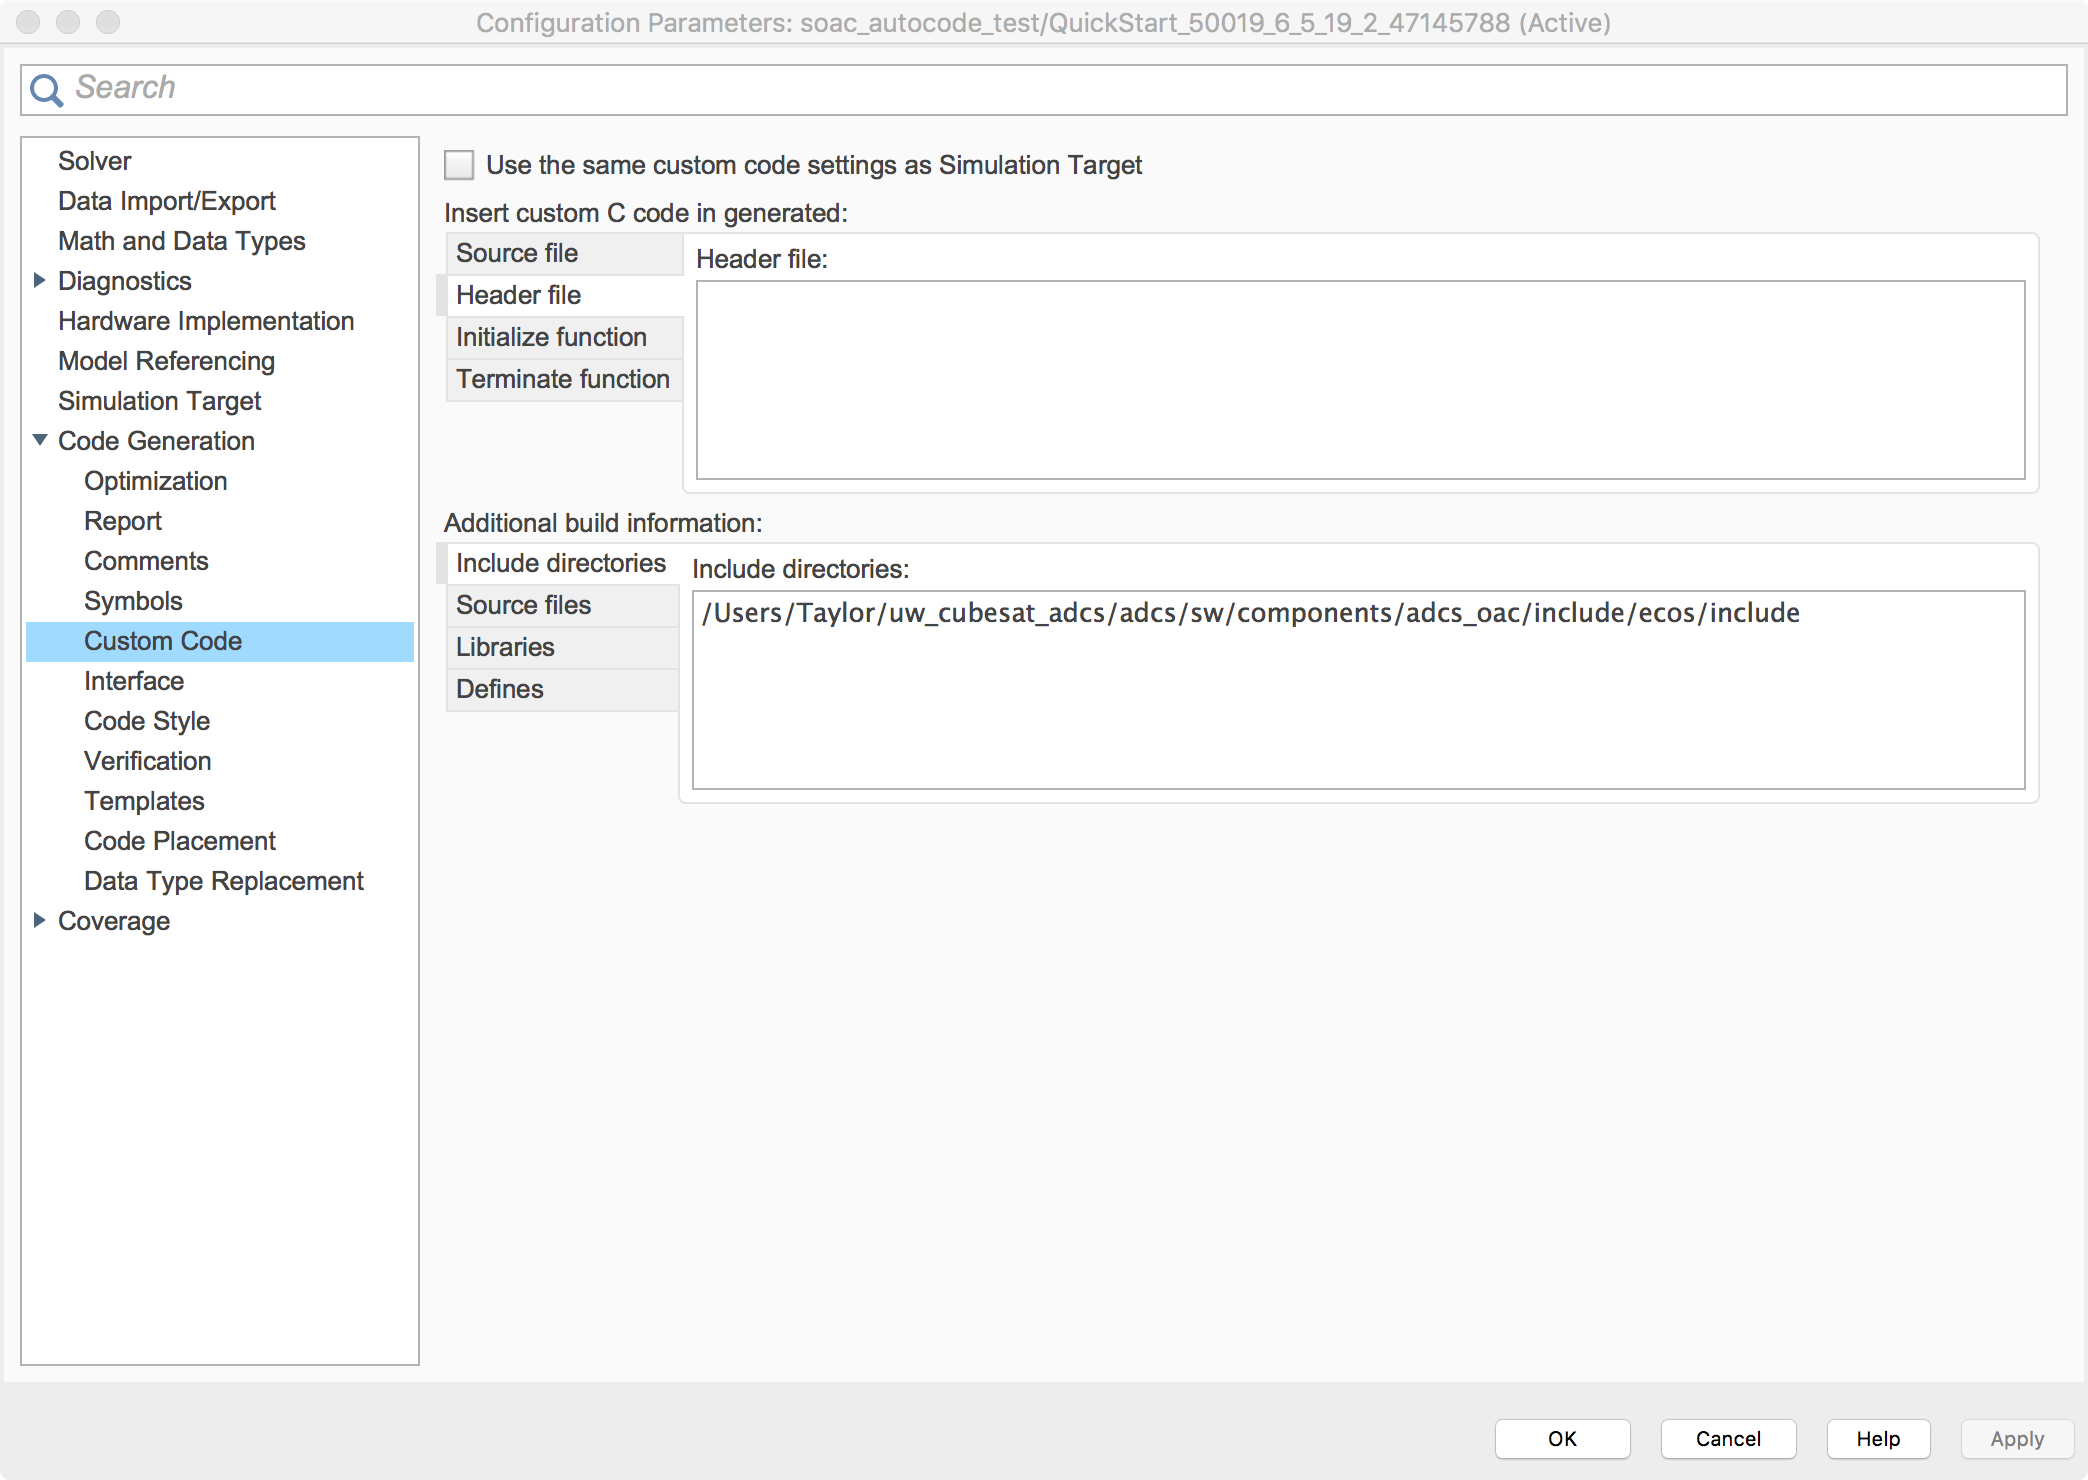
\includegraphics[width=0.85\textwidth]{figs/autocode_include.png}} \\
\subfloat{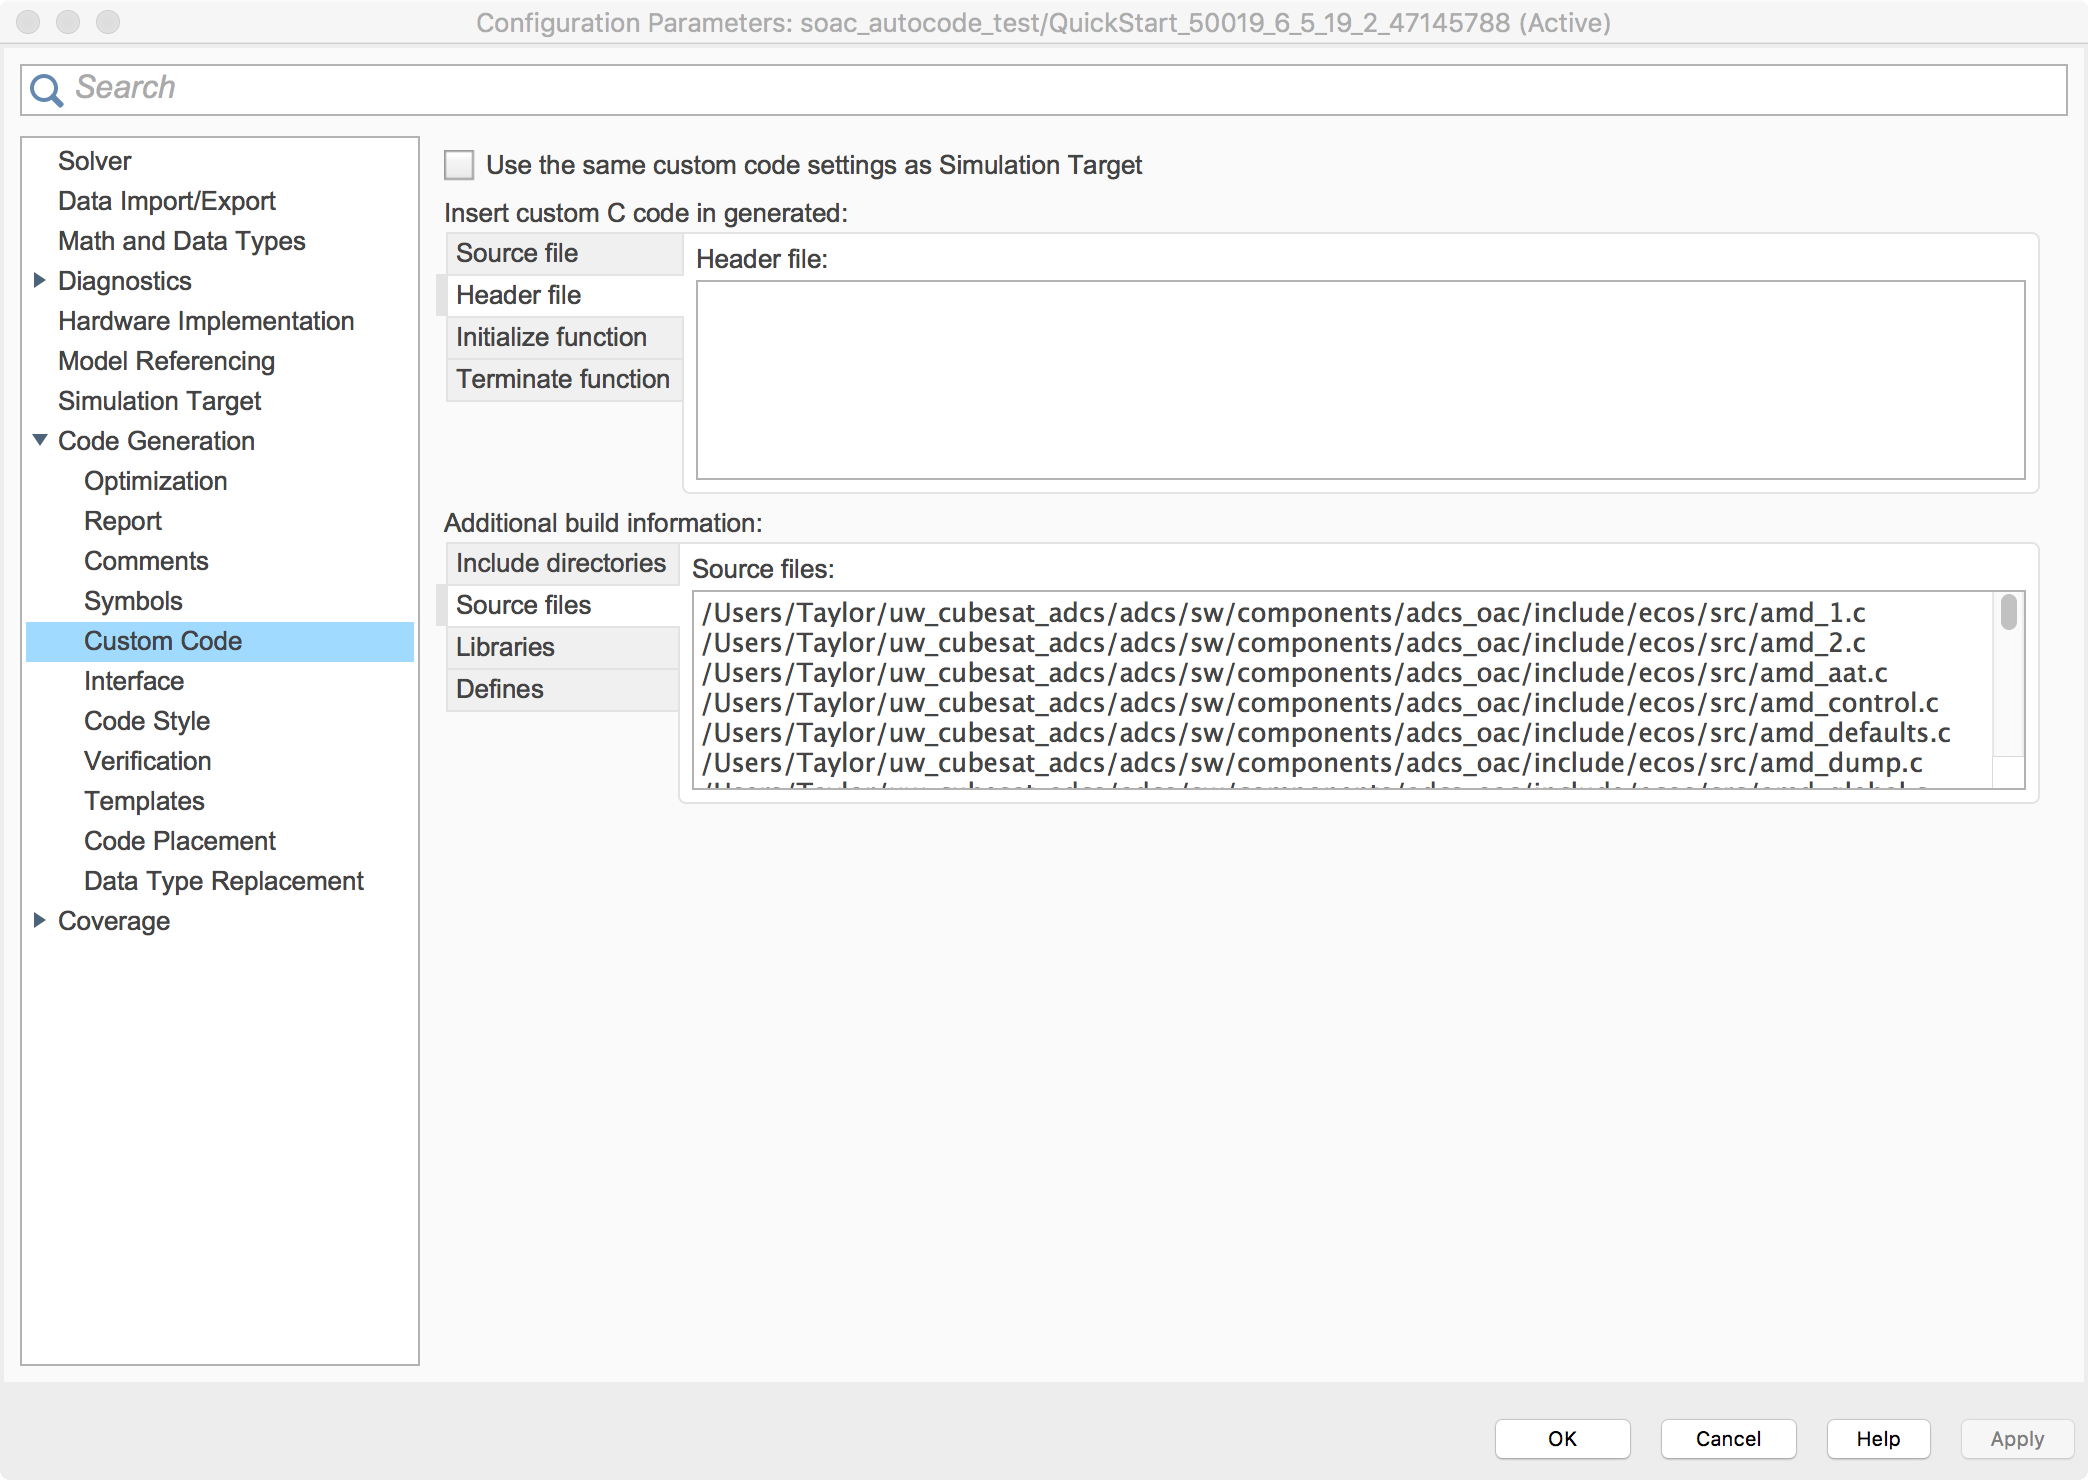
\includegraphics[width=0.85\textwidth]{figs/autocode_srcs.png}}
\caption{The custom code options found in Simulink's Code Generation Options.}
\label{fig:autocode}
\end{figure}

% Provide a functional block diagram of the system here. What is the main function of this system, what does it do? What are the inputs/outputs? How does information/power/etc. flow from input to output? What are the operating modes of your system, and how do they relate to the operating modes described in the Concept of Operations? You can break it down as much as you need here to give sufficient detail as to how your system operates. This is your chance to go into detail about how you have organized things to solve the problem you formulated in the summary section.  You should produce a state diagram (example here) detailing in plain english how your system will operate in every possible scenario.

\subsection{Mechanical Interface}\label{sec2:mech_interface}

The SOAC payload is a software function that will be run on the main flight computer. There is no separate mechanical interface.

\subsection{Electrical Interface}\label{sec2:elec_interface}

The SOAC payload is a software function that will be run on the main flight computer. There is no separate electrical interface.

\subsection{Command and Data Interface}\label{sec2:cmd_interface}

All inputs listed in~\tabref{tab:inputs_outputs} will come from the main GNC flight software. Refer to \href{https://drive.google.com/open?id=1wTjmsQdXGk9jmEHy59fZAdBJJ3r1IE4LGFjHT2S5png}{main GNC ICD}.

The output \ttt{soac\_solution} must be saved for future downlink to the ground station. This has been included in the COM system's measurement budget, and shall be maintained by CDH immediately once it is made available by SOAC. The two remaining outputs are to be provided as the GNC guidance solution and feed forward to the feedback controller that is used during primary GNC mode $33$. 

\subsection{Thermal Interface}\label{sec2:thermal_interface}

The SOAC payload is a software component that will be run on the main flight computer. There is no separate thermal interface. However, running the SOAC payload may cause an marked increase in the flight computer's computational load, and therefore it may produce more heat than nominal operating conditions. By calling SOAC only once (instead of repeatedly, see~\sref{sec3:op_modes}) it is hoped that SOAC will not create a large difference in thermal properties than what is expected for the main flight computer.

\section{Verification and Validation}\label{sec:v_and_v}

This section outlines the testing campaign that SOAC has so far passed during design, as well as a test case that can be used to assess correct functionality during a bench test. The following tests have been made:
\begin{enumerate}
\item A unit test of just the SOLVE function, found in the folder 
\begin{center}
\ttt{.../adcs\_oac/test/soac\_unit\_test}
\end{center}
\item A unit test of the entire SOAC library, found in the folder
\begin{center}
\ttt{.../adcs\_oac/test/soac\_interface\_unit\_test}
\end{center}
\item A Monte Carlo test of the entire SOAC library, found in the folder
\begin{center}
\ttt{.../adcs\_oac/test/soac\_mc\_test}
\end{center}
\end{enumerate}
Each folder contains a Matlab script and a Simulink library. Running the Matlab script will run the test and plot some results. The other test folders are not unit tests of the SOAC library in its Simulink form and can be ignored at this point (they were mostly used for development). 

A 1000 trial Monte Carlo test was run to assess the performance of the SOAC library at the preliminary design stage. The commanded attitude and angular rates were set to $\q_{cmd} = (1,0,0,0)$ and $\bm{\omega}_{\body,cmd}=(0,0,0)$ for each trial. The initial attitude was chosen by selecting a random direction on the unit sphere as an eigenaxis, and a error angle uniformly sampled from the interval $[-90\dg,90\dg]$. The initial quaternion is then
\begin{equation}
\theta \sim \mathcal{U}(-90\dg,90\dg), \quad \hat{\bm{n}} = \frac{(x,y,z)}{\|(x,y,z)\|}, \ x,y,z\sim\mathcal{N}(0,1), \quad \q(\ti) = \big(\cos(\tfrac{\theta}{2}),\,\sin(\tfrac{\theta}{2})\hat{\bm{h}} \big)
\end{equation} 
The initial attitude rates were chosen from
\begin{equation}
\wB(\ti) \sim \mathcal{N}(\zeros{3}{1},\,\Sigma_{\omega}), \quad \Sigma_{\omega} = \diag{10^{-3},10^{-3},10^{-2}}
\end{equation}
and the initial reaction wheel spin rates (in units of RPM) were chosen from
\begin{equation}
\Omega(\ti) \sim \mathcal{N}(\Omega_0,\,\Sigma_{\Omega}), \quad \Omega_0 = \begin{bmatrix}
1000 \\ -1000 \\ 1000 \\ -1000
\end{bmatrix}, \quad \Sigma_{\Omega} = 50\eye{4}
\end{equation}
which was then mapped to $\hw(\ti)$ to serve as the initial condition. 

The result of a single trial was assessed first by the value of the \code{exitcode} from SOAC. If the $16$th entry was zero, the trial was deemed a success; any other value was deemed a failure, see Table~\ref{tab:exitcodes}. Next, the resulting feedforward control/state were integrated through the spacecraft's nonlinear equations of motion using the dynamics that are being used to design the primary GNC flight software. A notional feedback controller was added to provide a sense of the closed-loop capabilities. The total degree error \textit{at the end of the maneuver} (i.e., the optimal time $s^* = \tf^*$) between $\q(\tf^*)$ and $\q_{cmd}$ was computed using $\q_{err} = \q(\tf^*)^* \otimes\ q_{cmd}$ and
\begin{equation}
\theta_{err} = 2 \arccos \big( q_{err,0} \big).
\end{equation} 
This measures the attitude error at the end of the maneuver \textit{only}, and does not provide information as to how well the path was tracked for times $t\in[\ti,\tf^*]$. Small values of $\theta_{err}$ are necessary but not sufficient to indicate satisfactory performance. If $\theta_{err}$ is small and there is no constraint violation for any time $t\in[\ti,\tf^*]$, then the maneuver is satisfactory at the preliminary design stage. 

Key metrics from the 1000 trials are given in Table~\ref{tab:mc_results}, and are visualized in Figures~\ref{fig:mc_results_errs} and~\ref{fig:mc_results_state}. No constraint violations were observed during closed loop simulations, and all trials achieved a final degree error of less than $3.5\dg$, the required control error bound per \href{https://docs.google.com/document/d/1SgZlPZIc5EONQ8ZSHsm3SXJ8XMwuNXoFASMoSIeQAhw/edit#heading=h.ybip8qn9pig1}{GNC Requirement 4.2.10}.

\begin{table}
\centering
\caption{Monte Carlo results on 2014 MacBook Pro with a 2.2 GHz Intel Core i7 processor and 16GB RAM. Note that this is \textbf{not} flight hardware, so the timing values are not representative of OBC performance.}
\label{tab:mc_results}
\begin{tabular}{lc}
\textbf{Metric} & \textbf{Value} \\ \hline\hline
Total trials & 1000 \\
Successful trials & 1000 \\
Failed trials & 0 \\
Maximum degree error & $2.22\dg$\\ 
Median degree error & $0.4672\dg$ \\ 
Maximum solver time & $65.2~\unit{ms}$ \\
Median solver time & $19.3~\unit{ms}$\\
Maximum number of iterations & $13$\\
Median number of iterations & $4$
\end{tabular}
\end{table}

\begin{figure}
\centering
\subfloat[Initial and final angle distributions]{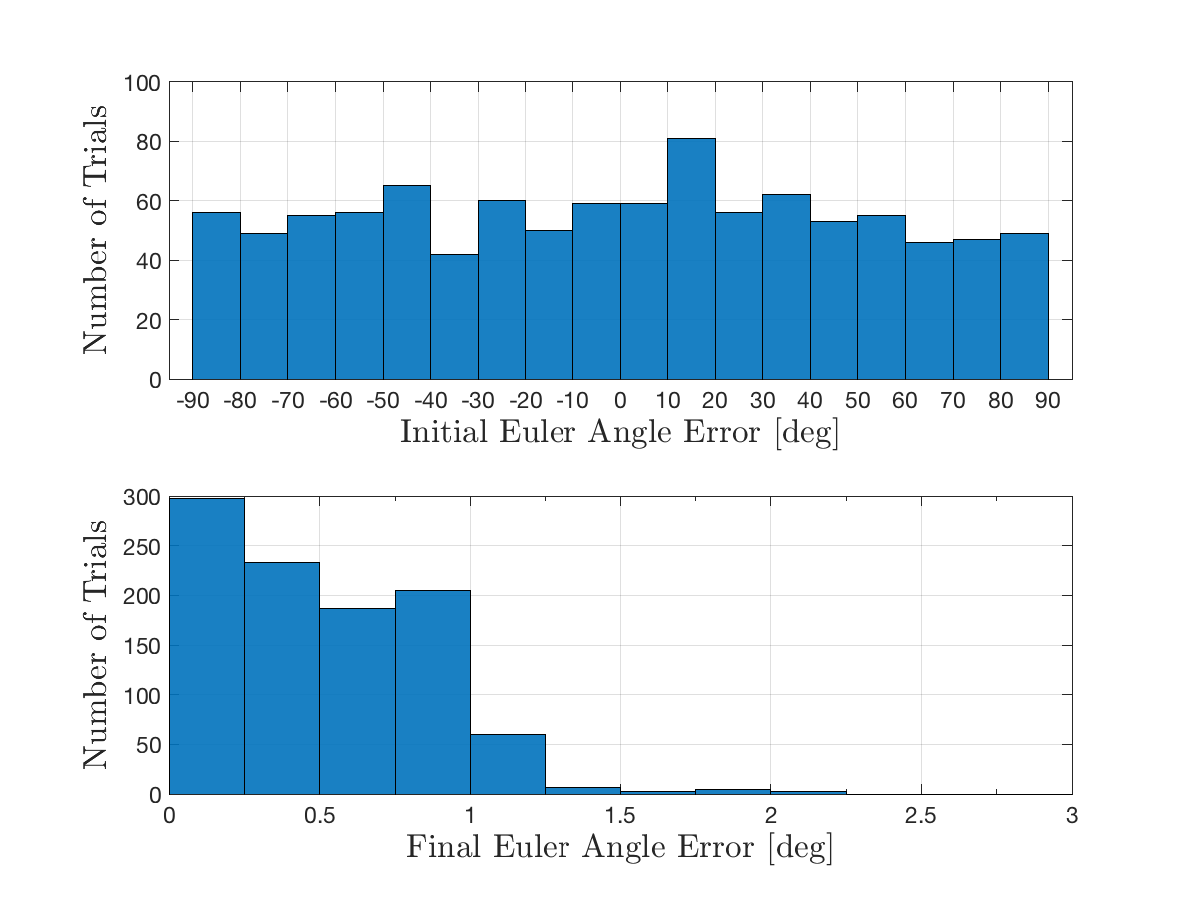
\includegraphics[width=0.75\textwidth]{figs/100219_dispersion_1000}}\\
\subfloat[Final versus initial angle errors]{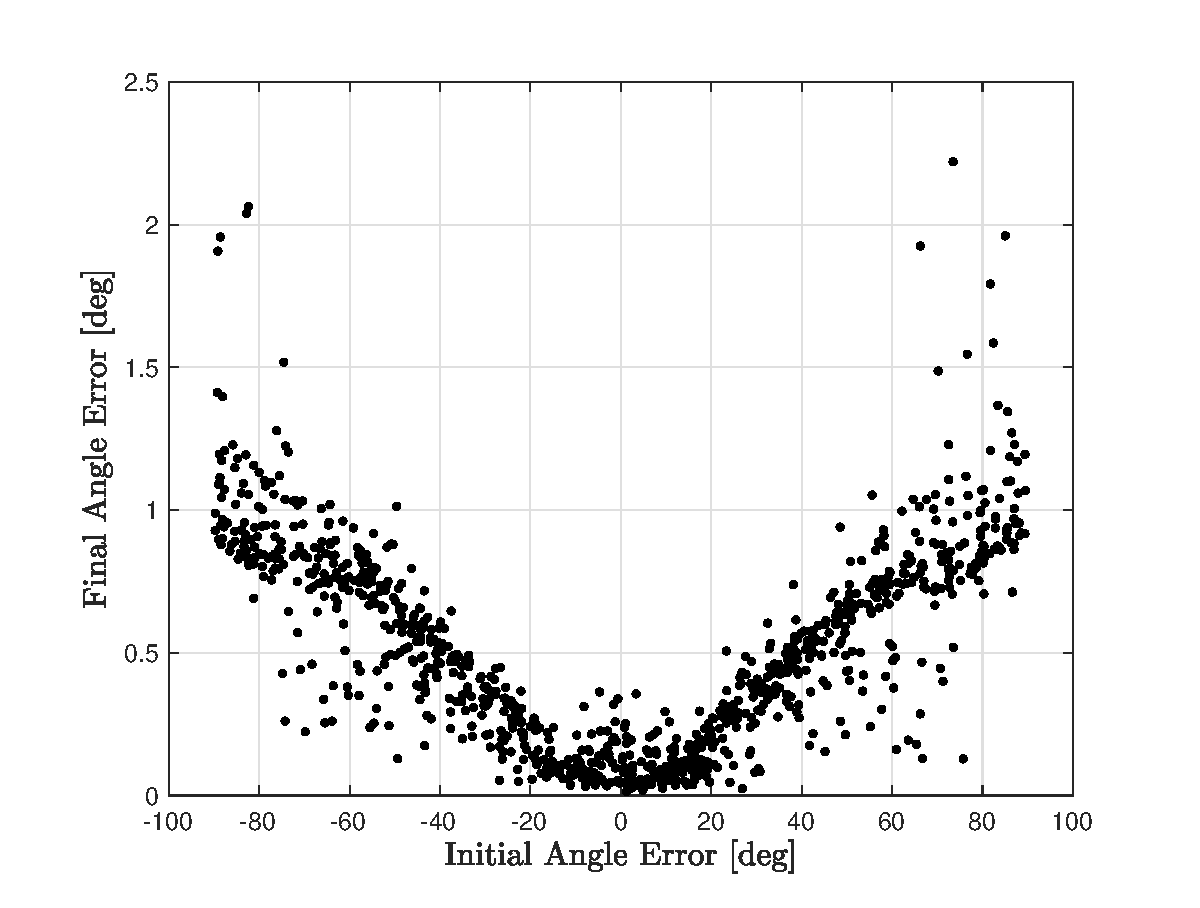
\includegraphics[width=0.75\textwidth]{figs/100219_mc_ic_fc_dispersion_1000}}
\caption{Closed loop results from 1000 randomized unit tests of SOAC. All final errors are within the required $3.5\dg$ control error bound.}
\label{fig:mc_results_errs}
\end{figure}

\begin{figure}
\centering
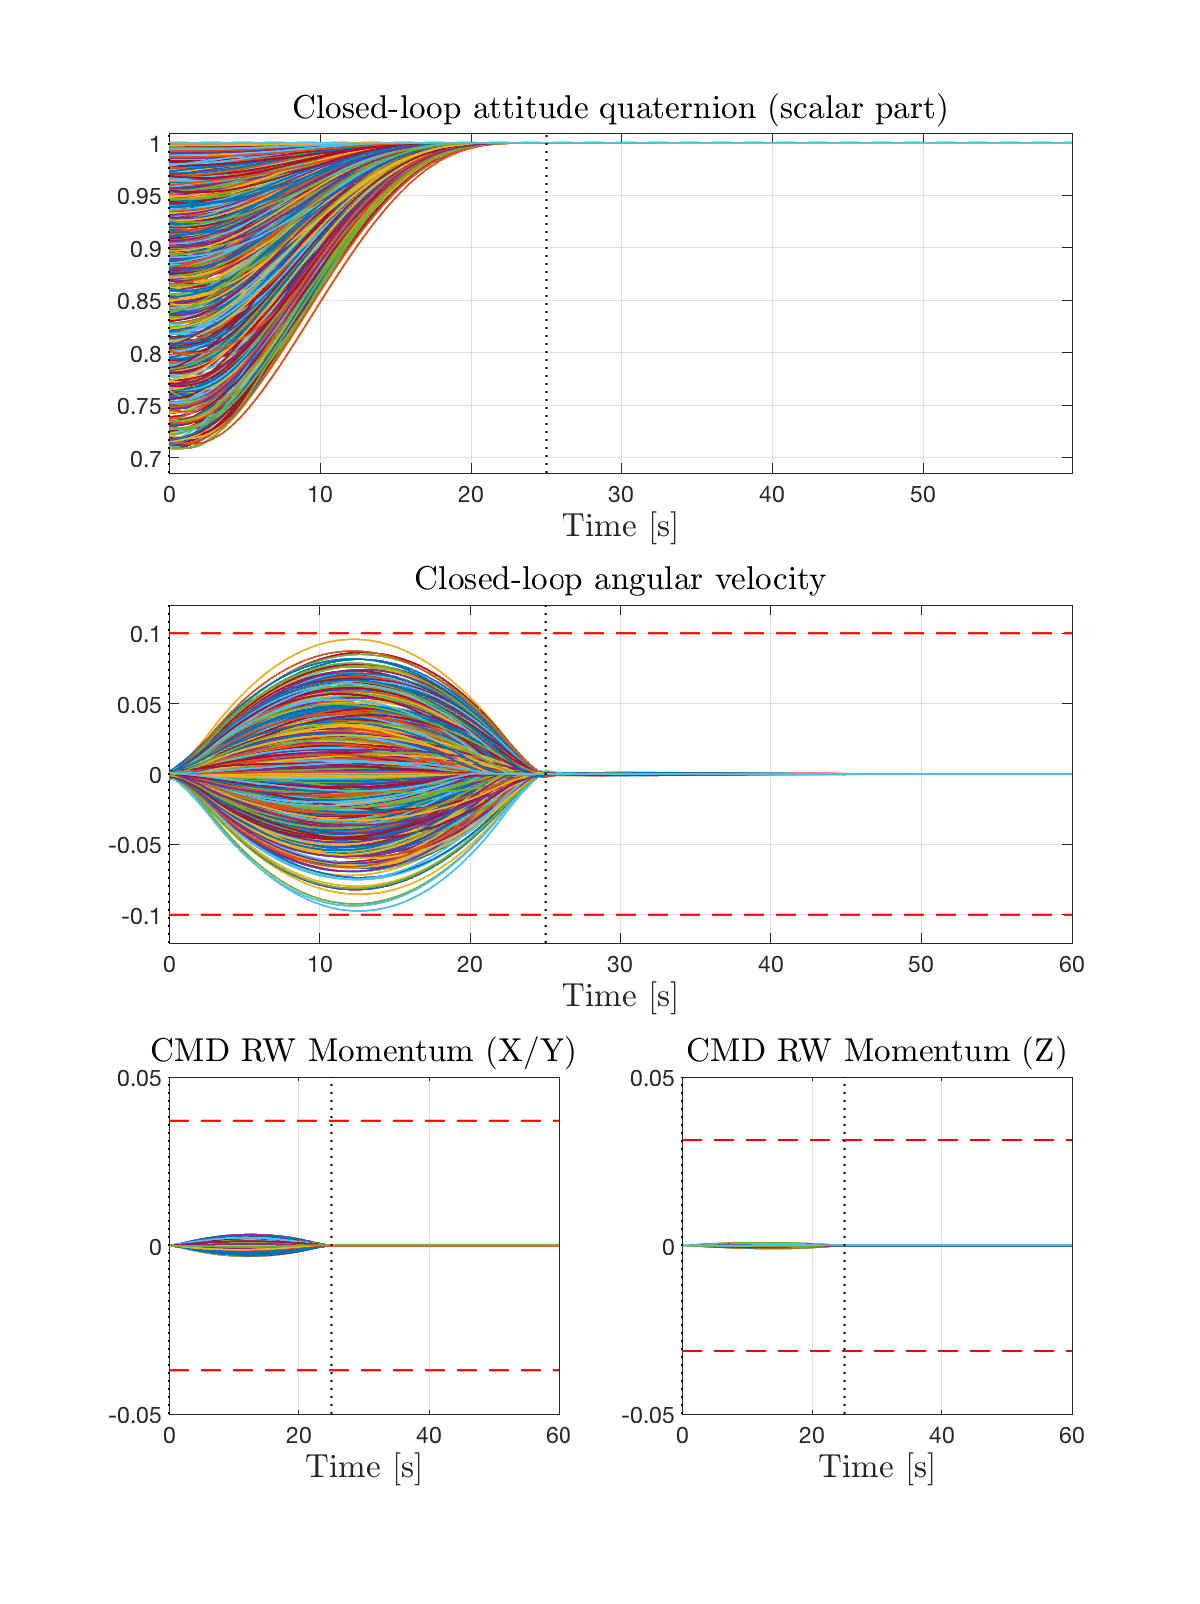
\includegraphics[width=0.75\textwidth]{figs/100219_mc_state_1000}
\caption{Closed loop results from 1000 randomized unit tests of SOAC. Dashed red lines indicate constraint boundaries.}
\label{fig:mc_results_state}
\end{figure}


\clearpage
\section*{Reference Tables}

\begin{table}[tbh]
\caption{Description of the SOAC payload's inputs and outputs}
\label{tab:inputs_outputs}
\centering
\begin{tabular}{ccccL{8cm}}
\multicolumn{5}{l}{\textbf{Inputs}}\\\hline\hline
\null & \textbf{Name} & \textbf{Size} & \textbf{Type} & \textbf{Description} \\ \hline
1 & \ttt{gnc\_mode} & \textit{scalar} & \code{int8} & The current GNC system operating mode. \\
2 & \ttt{quat\_ic}  & $4 \times 1$ & \code{double} & The current estimated attitude of the s/c. \\ 
3 & \ttt{w\_ic\_radps}  & $3 \times 1$ & \code{double} & The current estimated angular velocity of the s/c.\\
4 & \ttt{hw\_ic\_Nms} & $3 \times 1$ & \code{double} & The current momentum vector of the reaction wheels. \\
5 & \ttt{quat\_cmd} & $4 \times 1$ & \code{double} & The desired attitude at the end of the maneuver \\
6 & \ttt{w\_cmd\_radps} & $3 \times 1$ & \code{double} & The desired angular velocity at the end of the maneuver \\
7 & \ttt{sun\_inertial\_unit} & $3 \times 1$ & \code{double} & The inertial sun direction at the current time. This is assumed to be constant over the duration of the maneuver. \\
8 & \ttt{MET\_epoch} & \textit{scalar} & \code{double} & The maneuver epoch time in units of mission elapsed time (MET) provided via ground command prior to maneuver execution. \\
9 & \ttt{MET\_current} & \textit{scalar} & \code{double} & The current value of MET. \\~\\
\multicolumn{5}{l}{\textbf{Outputs}}\\\hline\hline
\null & \textbf{Name} & \textbf{Size} & \textbf{Type} & \textbf{Description} \\ \hline
1 & \ttt{soac\_telemetry} & $153\times 1$ & double & The entire output from the SOAC iterations. This should all be routed to ground for post-processing. See~Table~\ref{tab:soac_telemetry}.\\
2 & \ttt{command\_state} & $10\times 1$ & \code{double} & The interpolated state vector to be used as a reference for the feedback control system.\\
3 & \ttt{command\_torque} & $3\times 1$ & \code{double} & The interpolated control vector to be used as a feedforward actuator command.
\end{tabular}
\end{table}

\begin{table}[bht]
\caption{The components of the \code{soac\_telemetry} struct.}
\label{tab:soac_telemetry}
\centering
\begin{tabular}{ccc}
\textbf{Name} & \textbf{Size} & \textbf{Type} \\ \hline\hline
\code{opt\_state} & $100$ & \code{double} \\
\code{opt\_ctrl\_Nm} & $30$ & \code{double} \\
\code{final\_time\_s} & $1$ & \code{double} \\
\code{exitcode} & $17$ & \code{double} \\
\code{slv\_time\_s} & $15$ & \code{double} \\
\code{soac\_count} & $1$ & \code{uint32} \\
\end{tabular}
\end{table}

\begin{table}[bht]	
\caption{Possible values and meanings of \code{exitcode}.}
\label{tab:exitcodes}
\centering
\begin{tabular}{cL{11cm}}
\multicolumn{2}{l}{\textbf{From ECOS: Entries 1-15}}\\\hline\hline
\textbf{Value} & \textbf{Description} \\ \hline 
0 & Optimal solution found \\ 
1 & Certificate of primal infeasibility found \\
2 & Certificate of dual infeasibility found \\
10 & Optimal solution found subject to reduced tolerances \\
11 & Certificate of primal infeasibility found subject to reduced tolerances \\
12 & Certificate of dual infeasibility found subject to reduced tolerances \\
-1 & Maximum number of iterations reached \\
-2 & Numerical problems: unreliable search direction \\
-3 & Numerical problems: slacks or multipliers outside cone \\
-4 & Interrupted by signal or CTRL-C \\
-7 & Unknown problem in solver \\~\\
\multicolumn{2}{l}{\textbf{Custom: Entry 16}}\\\hline\hline
\textbf{Value} & \textbf{Description} \\ \hline 
1-15 & Number of global iterations taken \\~\\
\multicolumn{2}{l}{\textbf{Custom: Entry 17}}\\\hline\hline
\textbf{Value} & \textbf{Description} \\ \hline 
0 & All iterates found optimal solution and the terminal iterate meets the convergence criteria \\
-1 & One of the iterates did not return a 0 or 10 \\
3 & Maximum number of iterations reached: virtual control too large \\
4 & Maximum number of iterations reached: state change too large  
\end{tabular}
\end{table}


\clearpage
\section*{Appendix: Technical Details}

A general convex optimization problem is expressed
\begin{subequations}
\begin{align}
\min_{\bm{z}} &\quad f_0(\bm{z}) \\
\text{subject to:} &\quad h_i(\bm{z}) = 0, \quad i=1,\ldots,n_{eq} \\
&\quad f_j(\bm{z}) \leq 0, \quad j = 1,\ldots,n_{iq}
\end{align}
\end{subequations}
where $\bm{z}\in\real^{n_z}$ denotes the \textit{solution variable}, $f_0$ is the cost function, the $h_i$ are the \textit{equality constraints} and the $f_j$ are the \textit{inequality constraints}. The functions $f_j$ for $j=0,1,\ldots,n_{iq}$ must be \textit{convex functions} of the variable $\bm{z}$, while the functions $h_i$ for $i=1,\ldots,n_{eq}$ must be \textit{affine} functions of the variable $\bm{z}$.

\subsection*{Convex Cones}

Each proper cone $\coneK$ defines a \textit{generalized inequality} such that we may write $G \bm{z} \conleq h$ if and only if $h - G \bm{z} \in \coneK$. In particular we shall care about two cones, the \textit{linear cones} and the \textit{quadratic cones}. Linear cones are denoted by the set 
\begin{equation}
\lcone{n} = \{ \bm{z}\in\real^n \,|\, \bm{z} \geq 0 \},
\label{eq:lcone_set}
\end{equation}
where the inequality is understood elementwise. The other type of convex cones that we use are the second order cones, each of which are a set $\qcone{n+1}$ defined by
\begin{equation}
\qcone{n+1} = \big\{ (z_0,\bm{z}_n)\in\real\times\real^n \,|\, z_0 \geq \| \bm{z}_n \|_2 \big\}.
\label{eq:soc_set}
\end{equation}


To see how these are used to express various constraints as second order cone constraints, first note that a standard quadratic form is expressed as
\begin{equation}
\bm{x}^T A ^T A \bm{x} + b^T \bm{x} + c \leq 0
\label{eq:soc_quad}
\end{equation}
where $(A,b,c) \in \real^{n\times n} \times \real^n \times \real$ are constant constraint parameters. In standard form, this constraint is expressed by
\begin{equation}
\biggr\| \begin{bmatrix}
A \bm{x} \\ \frac{1}{\sqrt{2}}( 1 + c + b^T \bm{x} )
\end{bmatrix} \biggr\|_2 \leq \frac{1}{\sqrt{2}} ( 1 - b^T \bm{x} - c),
\label{eq:soc_std}
\end{equation} 
The proof of which follows from some straight-forward algebra. Now observe that according to the definition in~\eqref{eq:soc_set} we would like
\begin{equation*}
\begin{bmatrix}
\frac{1}{\sqrt{2}} ( 1 - b^T \bm{x} - c) \\
A \bm{x} \\
\frac{1}{\sqrt{2}} ( 1 + b^T \bm{x} + c)
\end{bmatrix} \in \qcone{n+2}
\end{equation*}
It should be clear that the first entry in the vector about is equivalent to $z_0$ in~\eqref{eq:soc_set}, and the remaining rows are equivalent to $\bm{z}_n$. Now, ECOS would like the matrix-vector pair $(G,h)$ such that $h-G\bm{x}\in\qcone{n+2}$, and so we set
\begin{equation}
h \definedas \begin{bmatrix}
\frac{1}{\sqrt{2}}( 1 - c ) \\ \zeros{n}{1} \\ \frac{1}{\sqrt{2}}(1+c)
\end{bmatrix} \quad G \definedas \begin{bmatrix}
\frac{b^T}{\sqrt{2}} \\ -A \\ -\frac{b^T}{\sqrt{2}}.
\end{bmatrix}
\end{equation}
The pair $(G,h)$ may be passed to ECOS to represent the quadratic constraint~\eqref{eq:soc_quad}.

\subsection*{Continuous Problem Formulation}

The continuous time optimal control problem to be solved in~\ref{prob:prob1} and is repeated here.
\begin{problem}\label{prob:prob1}
Find the time $\tf^*\in\realpp$ and torque commands $\bm{\tau} : [\ti,\tf^*] \rightarrow \real^3$ such that
\begin{subequations}
\begin{align}
\min_{\tf,\bm{\tau}(\cdot)} &\quad \int_{\ti}^{\tf^*} \bm{\tau}\tran\bm{\tau} dt \label{eq:prob_cost}\\
\text{subject to} &\quad \qdot = \frac{1}{2} \q \otimes \wB \label{eq:prob_b}\\
&\quad \dhB = \bm{\tau} + (\hB+\hw)^{\times} \left( \inv{J} \hB \right)\label{eq:prob_c}\\
&\quad \dhw = -\bm{\tau} \\
&\quad \| \wB \|_{\infty} \leq \wmax \label{eq:prob_d}\\
&\quad \| \uB \|_{\infty} \leq \umax \label{eq:prob_e}\\
&\quad \q^T \ME \q < 2 \label{eq:prob_f}\\
&\quad \q^T \MI \q < 2 \label{eq:prob_g}\\
&\quad \tfmin \leq \tf \leq \tfmax \label{eq:prob_h}\\
&\quad \q(\ti) = \qic,\quad \wB(\ti)=\wic,\quad \hw(\ti)=\hwic, \\
&\quad \q(\tf) = \q_f,\quad \wB(\tf) = 0.\label{eq:prob_i}
\end{align}
\end{subequations}
\end{problem} 

\subsection*{Transcription to Second-Order Cone Program}
This section details the steps necessary to obtain a convex second-order cone approximation of~\ref{prob:prob1} that is solved repeatedly, until convergence, within the SOLVE block of~\fref{fig:soac_inner}.

\paragraph{Time Normalization}
We define our \textit{state} to be $\bm{x} = \big[ \q \; \wB \big]^T \in \real^7$ and our \textit{control} to be $\bm{u} = \uB \in \real^3$. The dynamics in~\eqref{eq:prob_b} and~\eqref{eq:prob_c} can then be expressed in general using
\begin{equation}
\dot{\bm{x}}(t) = f(\bm{x},\bm{u}), \quad t \in [\ti,\tf].
\label{eq:dynamics_general}
\end{equation}
Since we are solving for the maneuvers final time, we must map the free-final time problem in Problem~\ref{prob:prob1} to a fixed-final time problem. We do so by defining a \textit{normalized time} $\tau\in[0,1]$ and changing our dynamics~\eqnref{eq:dynamics_general} to be
\begin{equation}
\der{\bm{x}}{t} = \der{\bm{x}}{\tau}\der{\tau}{t} = f(\bm{x},\bm{u}) \quad \Rightarrow \quad \der{\bm{x}}{\tau} = \der{t}{\tau} f(\bm{x},\bm{u})
\label{eq:dynamics_normalized}
\end{equation}
where $s \definedas \der{t}{\tau}$ is called the \textit{time-scaling factor}. By including $s$ as a solution variable, we can recover the final time for the maneuver using the relation $t_f = s \tau_f$. Since $\tau_f = 1$ by definition, we see that $s = t_f$. I use $s$ to keep the equations looking nicer.

\paragraph{Linearization}
The dynamics are linearized about a reference trajectory so that they are an affine function of the solution variables. Let's assume that we have access to a reference trajectory $\zb(\tau) \definedas \big(\xb(\tau),\,\ub(\tau),\,\sb\big)$ for $\tau\in[0,1]$. The first order Taylor series about $\zb(\tau)$ is then
\begin{subequations}\label{eq:linearization}
\begin{align}
\der{\xx}{\tau} &\approx \sb f(\xb,\ub) + A(\zb(\tau)) \big(\xx(\tau)-\xb(\tau) \big) + B(\zb(\tau)) \big( \uu(\tau) - \ub(\tau) \big) + S(\zb(\tau)) \big( s - \sb \big) \\
&= A(\zb) \xx + B(\zb) \uu + S(\zb) s + Z(\zb)
\end{align}
\end{subequations}
where,
\begin{subequations}
\begin{align}
A(\zb) &\definedas \der{}{\xx} s f(\xx,\uu) = s \begin{bmatrix}
A_{11} & A_{12} & \zeros{4}{3} \\
\zeros{3}{4} & A_{22} & A_{23} \\
\zeros{3}{4} & \zeros{3}{3} & \zeros{3}{3}
\end{bmatrix} \\
B(\zb) &\definedas \der{}{\uu} s f(\xx,\uu) = s \begin{bmatrix}
\zeros{4}{3} \\ -\eye{3} \\ \eye{3}
\end{bmatrix} \\
S(\zb) &\definedas \der{}{s} s f(\xx,\uu) = f(\xb,\ub) \\
Z(\zb) &\definedas - A(\zb) \xb - B(\zb) \ub 
\end{align}
\end{subequations}
and,
\begin{equation*}
A_{11} = \frac{1}{2} \begin{bmatrix}
0  & -\wB\tran  \\ \wB & \wB^{\times}
\end{bmatrix}, \quad A_{12} = \frac{1}{2}\begin{bmatrix}
-\qv\tran \\ \qv^{\times} + \qs \eye{3}
\end{bmatrix} \inv{J}, A_{22} = \left(\hB^{\times}+\hw^{\times}\right)\inv{J} - \wB^{\times}, \quad A_{23} = - \wB^{\times}.
\end{equation*}

\paragraph{Discretization}

I've chosen to parameterize our control with piecewise linear basis functions after some preliminary testing against other methods. To discretize the dynamics (projecting into a finite dimensional space), first discretize time into $N$ evenly spaced intervals. For now we proceed with $N=10$. 
\begin{equation}
\ti < t_1 < \ldots < t_{N-1} < \tf
\end{equation}
and represent the discretized time points using $k \definedas t_k$. Now, instead of the \textit{continuous times} $t\in(\ti,\tf]$, we have the \textit{discrete times} $k\in\{\ti,\,t_1,\,\ldots,\,t_{N-1},\,\tf\}$.

The control signal is parameterized over each time interval as
\begin{equation}
\uu(\tau) = \frac{t_{k+1} - t}{t_{k+1}-t_k} \uu_k + \frac{t-t_k}{t_{k+1}-t_k} \uu_{k+1}, \quad k=1,\ldots,N-1.
\end{equation}
This expression linearly interpolates between $\uu_k$ and $\uu_{k+1}$. The continuous time input can now be represented using a finite number of vectors, namely the set $\{\uu_{k}\}_{k=1}^{N}$. This parameterization is depicted in~\fref{fig:ctrl_param}.

\begin{figure}
\centering
\caption{Depiction of the control signal parameterization. The red dots are the discrete control vectors $\uu_{k}$ for $k=1,\ldots,N$ proceeding left to right.}
\label{fig:ctrl_param}
\foh{0}{0}{2}
\end{figure}

I'm skipping a bunch of details, which can all be found in~\cite{SzmukReynolds2018,Reynolds2019b}, but the discretization method reformulates~\eqnref{eq:linearization} into the form
\begin{equation}
\xx_{k+1} = A_{d,k} \xx_{k} + B_{d,k}^- \uu_k + B_{d,k}^+ \uu_{k+1} + S_{d,k} s + R_{d,k} \quad \Rightarrow \quad \bm{X} = A \bm{X} + B \bm{U} + S s + \bm{R}
\label{eq:discrete_dynamics}
\end{equation}
where the matrices $\{A,B,S,R\}$ are computed by the function \code{foh.m} in the code. The equation to the right of the implication is simply a concatenation using stacked vectors $\bm{X},\,\bm{U}$ and s. The constraints in~\eqref{eq:prob_d}-\eqref{eq:prob_g} are all ``discretized'' by simply applying them at the discrete temporal nodes only. 

\paragraph{Virtual Control}

To guide the convergence process, we introduce a new term to address the issue of \textit{artificial infeasibility}. This stems from the fact that the linearization may produce an infeasible iteration if there does not exists some admissible control that satisfies~\eqref{eq:discrete_dynamics}. We augment the dynamics with a virtual control term that allows us to synthetically retain feasibility according to
\begin{equation}
\bm{X} = A \bm{X} + B \bm{U} + \bm{S} s + \bm{R} + \bm{V}
\label{eq:VC_discrete_dynamics}
\end{equation}
where $\bm{V}$ can be thought of as an unconstrained input that needn't respect the physical dynamics of the problem. We heavily penalize the use of virtual control (so that we only use it when absolutely necessary) by augmenting the cost function~\eqref{eq:prob_cost} with $\wv \| \bm{V} \|_1$. If $\bm{V}=0$, then satisfaction of~\eqref{eq:VC_discrete_dynamics} implies satisfaction of~\eqref{eq:discrete_dynamics}.

After these modifications, we have a convex parameter optimization problem that can be solved iteratively on-board the spacecraft. 

\begin{problem}\label{prob:prob2}
Find the final time $s$ and the control $\bm{U}\in\real^{3 \times N}$ such that
\begin{subequations}\label{eq:prob2}
\begin{align}
\min_{s,\gamma,\bm{U},\bm{X},\bm{V}} &\quad \gamma + \wv \| \bm{V} \|_1 \label{eq:p2_a}\\
\text{subject to:} &\quad \bm{X} = A \bm{X} + B \bm{U} + \bm{S} s + \bm{R} + \bm{V} \label{eq:p2_b}\\
&\quad \| H_h \bm{x}_k \|_{\infty} \leq \wmax, \quad k=1,\ldots,N \label{eq:p2_c}\\ 
&\quad \| \bm{u}_k \|_{\infty} \leq \umax, \quad k=1,\ldots,N \label{eq:p2_d}\\
&\quad \bm{x}_k\tran \Hq\tran \ME \Hq \bm{x}_k < 2, \quad k=1,\ldots,N \label{eq:p2_e}\\
&\quad \bm{x}_k\tran \Hq\tran \MI \Hq \bm{x}_k < 2, \quad k=1,\ldots,N \label{eq:p2_f}\\
&\quad \tfmin \leq s \leq \tfmax \label{eq:p2_g} \\
&\quad \bm{U}\tran\bm{U} \leq \gamma \label{eq:p2_cost} \\ 
&\quad \bm{x}_1 = \big[ \qic\tran \; \hBic\tran \; \hwic\tran \big]\tran, \; H_f \xx_N = \big[ \q_f\tran \; \zeros{1}{3} \tran \big]\tran \label{eq:p2_h}
\end{align}
\end{subequations}
where $\bm{X} = \big[ \bm{x}_1\tran \; \bm{x}_1\tran \; \ldots \; \bm{x}_{N}\tran ]\tran \in \real^{10N}$ and similarly for $\bm{U}\in\real^{3N}$. Moreover, $\Hq = \big[ \eye{4} \; \zeros{4}{6} \big]$, $H_h = \big[ \zeros{3}{4} \; \inv{J} \; \zeros{3}{3} \big]$ and $H_f = \big[ \eye{7} \; \zeros{7}{3} \big]$.
\end{problem}
The solutions to~\pref{prob:prob2} are used to re-discretize the nonlinear dynamics, producing a new set of matrices $\{A,B,S,R\}$, which are then used to re-solve~\pref{prob:prob2}.

\paragraph{Scaling}
The solution variables can be scaled for better numerical stability by using the diagonal matrices $D_x,\,D_u,\,D_s$ that are defined in the \code{init\_soac\_params.m} file. These are defined so that, for example, $\xx_k = D_x \hat{\xx}_{k}$, and the solver is asked to solve for $\hat{\xx}_k$ instead. The entries in $D_x$ can be chosen so that the expected range of $\hat{\xx}_k$ is roughly $[-1,1]$, providing better numerical conditioning. Sufficient performance has been observed without any scaling (i.e., setting all of these matrices to the identity). For the preliminary design, each matrix has been set to the identity matrix. \textit{If no scaling is required to successfully pass performance testing, these operations should be removed from the library as they would be useless algebraic operations that needlessly increase solution time.} 

\paragraph{Standard Form of Constraints}

Our combined \textit{solution vector} is 
\begin{equation*}
\bm{z} = \begin{bmatrix}
\bm{X}\tran & \bm{U}\tran & \gamma & s & \bm{V}\tran & \bm{\eta}_v\tran
\end{bmatrix} \in \real^{n_z}
\end{equation*}
where $n_z = N(3N_x + N_u)+2$. We will first map the cost function to standard form for second-order cone problems. The cost function must be linear, and so we will use the epigraph form to rewrite the cost function~\eqref{eq:p2_a} as
\begin{equation}
\bm{c}\tran \bm{z}, \qquad \bm{c} = \big[ \zeros{1}{10N} \ \zeros{1}{3N} \ 1 \ 0 \ \zeros{1}{10N} \ w_{\eta} \ones{10N} \big]
\label{eq:std_cost}
\end{equation}
and add the following linear constraint to Problem~\ref{prob:prob2}
\begin{equation}
- \bm{\eta}_v \leq \bm{V} \leq \bm{\eta}_v.
\label{eq:p2_epi}
\end{equation}

We can then write the equality constraints~\eqref{eq:p2_b} and~\eqref{eq:p2_h} in the form $A \bm{z} = \bm{b}$ using
\begin{equation}
\begin{bmatrix}
\big[ \eye{10} \ \zeros{10}{10(N-1)}] & \zeros{10}{3N} & \zeros{10}{1} & \zeros{10}{1} & \zeros{10}{10N} & \zeros{10}{10N} \\
\bm{A} - \eye{10N} & \bm{B} & \zeros{10N}{1} & \bm{S} & \eye{10N} & \zeros{10N}{10N} \\
\big[ \zeros{10}{10(N-1)} \ \eye{10} \big] & \zeros{10}{3N} & \zeros{10}{1} & \zeros{10}{1} & \zeros{10}{10N} & \zeros{10}{10N}
\end{bmatrix} \bm{z} = \begin{bmatrix}
\bm{x}_0 \\ -\bm{R} \\ \bm{x}_f
\end{bmatrix}
\label{eq:std_equality}
\end{equation}
The linear inequality constraints in~\eqref{eq:p2_c}, \eqref{eq:p2_d}, \eqref{eq:p2_g} and \eqref{eq:p2_epi} are expressed as
\begin{equation}
\begin{bmatrix}
H_w^T \\ - H_w^T \\ H_u^T \\ - H_u^T \\ H_s^T \\ - H_s^T \\ H_v^T - H_{\eta_v}^T \\ -H_v - H_{\eta_v}^T
\end{bmatrix} \bm{z} \leq \begin{bmatrix}
w_{\max} \ones{3N} \\ w_{\max} \ones{3N} \\ u_{\max} \ones{3N} \\ u_{\max} \ones{3N} \\ t_{f,\max} \\ -t_{f,\min} \\ \zeros{10N}{1} \\ \zeros{10N}{1}
\end{bmatrix} \quad \iff \quad G_{lin} \zz \leq \bm{h}_{lin},
\label{eq:std_ineq_lin}
\end{equation}
where,
\begin{gather*}
H_u = \begin{bmatrix}
\zeros{10N}{3N} \\ \eye{3N} \\ \zeros{(20N+2)}{3N}
\end{bmatrix}, \quad H_s = \begin{bmatrix}
\zeros{13N}{1} \\ 0 \\ 1 \\ \zeros{20N}{1}
\end{bmatrix}, \quad H_{\gamma} = \begin{bmatrix}
\zeros{13N}{1} \\ 1 \\ 0 \\ \zeros{20N}{1}
\end{bmatrix}, \quad H_v = \begin{bmatrix}
\zeros{(13N+2)}{10N} \\ \eye{10N} \\ \zeros{10N}{10N} 
\end{bmatrix}  \\
H_{\eta_v} = \begin{bmatrix}
\zeros{(23N+2)}{10N} \\ \eye{10N}
\end{bmatrix}, \quad
\bar{H}_w = \eye{N} \otimes \begin{bmatrix}
\zeros{3}{4} & J^{-1} & \zeros{3}{3}
\end{bmatrix}, \quad H_w = \begin{bmatrix}
\bar{H}_w \\ \zeros{(23N+2)}{3N} 
\end{bmatrix}
\end{gather*}

If there are no attitude exclusion/inclusion zone constraints, then the second-order cone constraint(s) are written as a function of $\bm{z}$ using
\begin{equation}
\begin{bmatrix}
-\frac{1}{\sqrt{2}}H_{\gamma}\tran \\ -H_u\tran \\ \frac{1}{\sqrt{2}} H_{\gamma}\tran
\end{bmatrix} \zz \leq \begin{bmatrix} 
\frac{1}{\sqrt{2}} \\ \zeros{3N}{1} \\ \frac{1}{\sqrt{2}}
\end{bmatrix} \quad \iff \quad G_{quad} \zz \leq \bm{h}_{quad}
\label{eq:std_b_quad}
\end{equation}
This cone has dimension $32$. 

For each $k=1,\ldots,N$, the attitude inclusion/exclusion constraints can be written using 
\begin{align*}
P_{i,k} = \tilde{M}_i H_q H_k  \quad &\text{and} \quad P_{e,k} = \tilde{M}_e H_q H_k \\
G_{i,k} = \begin{bmatrix}
\zeros{1}{n_z} \\ - P_{i,k} \\ \zeros{1}{n_z}
\end{bmatrix} \quad &\text{and} \quad G_{e,k} = \begin{bmatrix}
\zeros{1}{n_z} \\ -P_{e,k} \\ \zeros{1}{n_z}
\end{bmatrix} \\
\bm{h}_{i,k} = \begin{bmatrix}
\frac{3}{\sqrt{2}} \\ \zeros{4}{1} \\ -\frac{1}{\sqrt{2}}
\end{bmatrix} \quad &\text{and} \quad \bm{h}_{e,k} = \bm{h}_{i,k}
\end{align*}
where,
\begin{equation*}
H_{x_k} = \begin{bmatrix}
\zeros{10}{10} & \cdots & \underbrace{\eye{10}}_{k\text{th block}} & \cdots & \zeros{10}{10} & \zeros{10}{(23N+2)} \end{bmatrix}
\end{equation*}
Each of these cones have dimension 6. The quantities $G_{\cdot,k}$ and $h=\bm{h}_{\cdot,k}$ are appended to the bottom of $G_{quad}$ and $\bm{h}_{quad}$ as they are computed. The problem sizes are summarized in Table~\ref{tab:soac_dimensions}.

\begin{table}[tb!]
\centering
\caption{Maximum dimensions for the SOAC payload optimization problem. The function \code{convert\_to\_CCS} inside the SOLVE function maps a general matrix $M$ to the compressed column storage matrices $\{M_{jc},M_{ir},M_{pr}\}$ -- see~\cite{MalyutaThesis}.}
\label{tab:soac_dimensions}
\begin{tabular}{ccccl}
\textbf{Variable} & \textbf{Size} & \textbf{Type} & \textbf{Value} & \textbf{Description} \\ \hline\hline 
$n$ & $1$ & \code{int32} & $332$ & number of primal variables \\
$m$ & $1$ & \code{int32} & $474$ & number of generalized inequality constraints, rows of $G$ in~\eqref{eq:gen_inequalities} \\
$p$ & $1$ & \code{int32} & $117$ & number of equality constraints, rows of $A$ \\
$l$ & $1$ & \code{int32} & $322$ & number of linear inequality constraints, rows of $h_{lin}$ \\
$ncones$ & $1$ & \code{int32} & $21$ & number of second order cone constraints, rows of $h_{quad}$ \\ 
$\bm{c}$ & $332$ & \code{double} & see~\eqref{eq:std_cost} & cost vector \\
$G_{jc}$ & $333$ & \code{int32}  & \null & generalized inequality constraint matrix (part of CCS format) \\
$G_{ir}$ & $834$ & \code{int32}  & \null & generalized inequality constraint matrix (part of CCS format)\\
$G_{pr}$ & $834$ & \code{double} & \null & generalized inequality constraint matrix (part of CCS format)\\
$\bm{h}$ & $474$	& \code{double} & see~\eqref{eq:gen_inequalities} & generalized inequality constraint vector \\
$q$ & $21$ & \code{int32} & \null & dimensions of each second order cone. Size m \\
$A_{jc}$ & $333$ & \code{int32} & \null & equality constraint matrix (part of CCS format) \\
$A_{ir}$ & $1278$ & \code{int32} & \null & equality constraint matrix (part of CCS format)\\ 
$A_{pr}$ & $1278$ & \code{double} & \null & equality constraint matrix (part of CCS format)\\
$\bm{b}$ & $117$	& \code{double} & see~\eqref{eq:std_equality} & equality constraint vector
\end{tabular}
\end{table}

The inequality constraints are then passed to ECOS using the data
\begin{equation}
G = \begin{bmatrix}
G_{lin} \\ G_{quad}
\end{bmatrix}, \quad \bm{h} = \begin{bmatrix}
\bm{h}_{lin} \\ \bm{h}_{quad}
\end{bmatrix} \quad \Rightarrow \quad G \bm{z} \leq \bm{h}, \quad \text{and} \quad q = \begin{bmatrix}
32 \\ 6\,\ones{2N}
\end{bmatrix}.
\label{eq:gen_inequalities}
\end{equation}
Note that $q$ is the ECOS input that provides the second order cone dimensions, and has length $\code{ncones} = 2N+1$. The standard form of~\pref{prob:prob2} is then simply

\begin{problem}
Find the vector $\bm{z}\in\real^{n_z}$ such that
\begin{subequations}\label{eq:prob2}
\begin{align}
\min_{\bm{z}} &\quad \bm{c}^T \bm{z} \tag{\ref{eq:std_cost}}\\
\text{subject to:} &\quad A \bm{z} = \bm{b} \tag{\ref{eq:std_equality}} \\
&\quad G \bm{z} \preceq_{\mathcal{K}} \bm{h} \tag{\ref{eq:gen_inequalities}}
\end{align}
\end{subequations}
\end{problem}
where the generalized inequality is either a linear cone as in~\eqref{eq:lcone_set} or a second order cone as in~\eqref{eq:soc_set}. Which one applies to which entries of $G$ and $\bm{h}$ is controlled by the value of $l$ and $ncones$. Always the first $l$ rows of $G$ are linear cones, and the next $sum(q)$ rows are second order cones of dimension $q(k)$.

% \subsubsection{Compressed Column Storage}

% \todo{add a section that discusses compressed column storage (ref. Danylo's thesis).}
\bibliographystyle{plain}
\bibliography{soacbib}

\end{document}